\chapter{Causal inference}\label{chap12}

In this chapter, we present some Bayesian methods to perform inference on \textit{causal} effects. The point of departure is \textit{identification conditions} which are the set of assumptions that allow us to express the \textit{estimand} —the causal or statistical quantity of interest— as a unique function of the observable data distribution. These identification conditions are conceptually distinct from the econometric or statistical framework used to perform inference once those conditions are satisfied. In other words, the assumptions necessary for identification do not constrain whether we apply a Frequentist or a Bayesian approach for estimation and inference.

Identification addresses the question: \textit{Can the causal effect be expressed as a function of the observable data distribution under certain assumptions?} Once the causal effect is identified in terms of the observed data distribution, we can proceed with statistical inference using either Frequentist methods or Bayesian methods. These inferential frameworks differ in how they estimate and quantify uncertainty but operate on the same identified causal effect. Thus, the identification assumptions are logically prior and independent of whether we adopt a Frequentist or a Bayesian inferential paradigm.

Thus, we present the underlying identification assumptions employed in popular strategies such as randomized controlled trials, conditional independence, and instrumental variables, among others, as well as the Bayesian inferential framework used to estimate causal effects in these settings. 

We should be clear that this is only an introduction to causal inference, and we do not aim to provide an in-depth discussion. There are excellent texts on causal inference, such as \cite{angrist2009mostly,angrist2014mastering,imbens2015causal,hernan2020causal,cunningham2021causal,chernozhukov2024applied}. We recommend that readers consult these references for a deeper understanding of some of the concepts and tools introduced in this chapter.

\section{Identification setting}\label{chap12_1}

The aim is to identify the \textit{causal} or \textit{treatment effect} of a particular regressor or treatment on an outcome. For example, this could involve estimating the causal effect of a labor training program on individuals’ earnings or unemployment, or the price elasticity of demand. The starting point is the \textit{potential outcomes} framework \cite{rubin1974}, which defines a \textit{counterfactual scenario} describing what would happen to the outcome variable if the treatment status or level were different (commonly referred to as the \textit{Rubin causal model} \cite{holland1986statistics}).

In this context, \textit{treatment status} refers to a binary treatment case with two potential outcomes; for instance, what would my earnings be if I had participated in the training program? Conversely, \textit{treatment level} applies to cases where there is a potential outcome for each level of the treatment; for example, what would demand be if the price had increased by 10\%?

Following the potential outcomes notation in the binary treatment case, let $D_i = 1$ and $D_i = 0$ indicate the treatment status, corresponding to \textit{treated} and \textit{control} units, respectively. The potential outcomes $Y_i(1)$ and $Y_i(0)$ represent the outcome for unit $i = 1, 2, \dots, N$ under treatment and control, respectively. For instance, $Y_i(1)$ denotes the employment status an individual would have if she/he would have participated in the training program, regardless of their actual participation, whereas $Y_i(0)$ denotes the employment status if the individual would not have attended the program. The individual-level treatment effect is then defined as
\begin{align*}
	\tau_i = Y_i(1) - Y_i(0).
\end{align*}

The potential outcomes framework can also be extended to situations where the treatment is continuous \cite{imbens2014ivperspective}. In this case, let $Y_i(x_s)$ denote the outcome for unit $i$ under the counterfactual scenario where the treatment variable $X_s$ takes the value $x_s$. The ``treatment effect'' of changing $X_s$ from $x_s$ to $x_s'$, for example, the effect of increasing the price by 10\% on demand, is given by
\begin{align*}
	\beta_{si} = Y_i(x_s') - Y_i(x_s).
\end{align*}
When the change is infinitesimal, the causal effect can be expressed as a marginal effect:
\begin{align*}
	\beta_{si} =\frac{\partial Y_i(x_s)}{\partial x_s}.
\end{align*}
This setting is more complex than the binary treatment case because there is a potential outcome for each possible value of $x_s$ \cite{gill2001causal}. Therefore, we begin by considering the binary treatment case. However, \textit{the fundamental problem of causal inference} \cite{holland1986statistics} remains: it is impossible to observe the same unit under different \textit{treatment statuses} simultaneously. Consequently, we must learn about causal effects by comparing the outcomes of treated and untreated units.

Bayesian inference for causal effects \cite{rubin1978bayesian} is more direct than procedures based on Fisher's \textit{p}-value approach, which relies on the logic of stochastic proof by contradiction, or Neyman's randomization-based inference, which is grounded in the idea of repeated sampling and the construction of confidence intervals for treatment effects \cite{rubin2004teaching}.

Bayesian inference for causal effects treats the potential outcomes as random variables and involves computing the posterior predictive distribution to evaluate treatments not received, conditional on the observed responses to treatments actually received. This approach yields the posterior distribution of the causal estimands as a function of both the observed outcomes and the unobserved potential outcomes, which are treated as missing data and handled through data augmentation methods \cite{Tanner1987}. 

In addition, it is important to note that the likelihood function does not contain information about the correlation between potential outcomes due to \textit{the fundamental problem of causal inference}. Consequently, most of the classical literature on treatment effects has focused on average treatment effects, which require only the marginal distributions of the potential outcomes $Y(1)$ and $Y(0)$ \cite{heckman2014treatment}. Nevertheless, it is also possible to estimate \textit{quantile treatment effects} \cite{AbadieAngristImbens2002,Chernozhukov2005}.  

There are also Bayesian proposals for performing inference on the correlation between potential outcomes \cite{koop1997learning,heckman2014treatment}. These approaches allow recovery of the joint distribution of the potential outcomes, thereby enabling inference beyond average treatment effects. However, this requires learning from the prior rather than the data, or imposing additional structure on the causal model.  

A Bayesian framework further makes it possible to estimate \textit{distributional treatment effects} with uncertainty quantification, as formally defined by \cite{aakvik2005estimating}. See also \cite{heckman2014treatment} for related proposals. These effects also characterize the entire distribution of potential outcomes under treatment and control, rather than focusing solely on averages, thereby capturing heterogeneity. This is particularly relevant for policy, as it enables estimation of the proportion of the population that benefits from a social program or the probability that a treated individual experiences a positive effect \cite{heckman2014treatment,Ramirez2019a}.

Furthermore, under a Bayesian framework, the impact of adding or relaxing identification assumptions can be assessed by examining how the distributional treatment effects change \cite{imbens1997bayesian}.

\section{Randomized controlled trial (RCT)}\label{chap12_2}

Two of the most relevant estimands in the causal inference literature are the average treatment effect (ATE),
\[
\text{ATE} = \mathbb{E}[Y_i(1) - Y_i(0)],
\]
and the average treatment effect on the treated (ATT),
\[
\text{ATT} = \mathbb{E}[Y_i(1) - Y_i(0) \mid D_i = 1].
\]

However, these estimands are not directly identifiable without additional assumptions because we never observe the same unit under both treatment states simultaneously. Therefore, identification restrictions are required to express these causal quantities in terms of the observed data.

Note that the observed mean difference between treated and untreated units can be decomposed as:
\begin{align*}
\mathbb{E}[Y_i \mid D_i = 1] - \mathbb{E}[Y_i \mid D_i = 0] 
& = \underbrace{\mathbb{E}[Y_i(1) - Y_i(0) \mid D_i = 1]}_{\text{ATT}}\\
& + \underbrace{\Big( \mathbb{E}[Y_i(0) \mid D_i = 1] - \mathbb{E}[Y_i(0) \mid D_i = 0]\Big)}_{\textit{Selection Bias}},
\end{align*}

that is, the observed mean difference equals the ATT plus the \textit{selection bias}, which captures the difference between the expected potential outcome of treated individuals had they not been treated (unobserved) and the expected outcome of untreated individuals (observed). 

The sign of the selection bias depends on the nature of self-selection into treatment. Two illustrative examples are:

\begin{table}[H]
	\caption{Illustrative examples of selection bias}
	\begin{minipage}{0.5\textwidth} % Adjust width as needed
		
		\begin{tabular}{lccc}
			\hline
			\textbf{Scenario} & $\mathbb{E}[Y(0)\mid D=1]$ & $\mathbb{E}[Y(0)\mid D=0]$ & Selection Bias \\
			\hline
			\textit{Training Program} & 80 & 70 & $+10$ \\
			\textit{Remedial Education} & 60 & 70 & $-10$ \\
			\hline
		\end{tabular}
	\end{minipage}
\end{table}

In the first scenario, motivated individuals self-select into a training program and would have higher earnings even without participation, producing a positive selection bias and causing the observed mean difference to overestimate the ATT. In the second scenario, disadvantaged individuals are more likely to enroll in a remedial education program and would have lower outcomes without the program, resulting in a negative selection bias and causing the observed mean difference to underestimate the ATT.

Note that if we assume that \textit{assignment to treatment is random},
\[
\{ Y_i(1), Y_i(0) \} \perp D_i,
\]
then the selection bias becomes zero,
\[
\mathbb{E}[Y_i(0) \mid D_i = 1] - \mathbb{E}[Y_i(0) \mid D_i = 0] = 0,
\]
which means there is no selection bias under random assignment.

Moreover, under random assignment, ATT equals ATE:
\[
\tau = \underbrace{\mathbb{E}[Y_i(1)\mid D_i=1]-\mathbb{E}[Y_i(0)\mid D_i=1]}_{\text{ATT}} 
= \underbrace{\mathbb{E}[Y_i(1)-Y_i(0)]}_{\text{ATE}}.
\]
Consequently,
\begin{equation}
	\tau=\mathbb{E}[Y_i \mid D_i = 1] - \mathbb{E}[Y_i \mid D_i = 0],
\end{equation}

that is, the average causal effect is function of the data under random assignment to treatment.
 
\textit{Randomized controlled trials} (RCTs) are characterized by \textit{random assignment to treatment}. The identification of causal effects in RCTs additionally relies on two key assumptions: \textit{overlap}, which requires that every unit has a positive probability of being assigned to both treatment and control groups ($0 < P(D_i = 1) < 1$), and the \textit{Stable Unit Treatment Value Assumption} (SUTVA). The latter consists of two components: (i) \textit{no interference}, meaning one unit’s potential outcome is unaffected by another unit’s treatment, and (ii) \textit{consistency}, meaning the observed outcome equals the potential outcome corresponding to the received treatment.

We can represent the causal mechanism in an RCT using \textit{causal diagrams} \cite{pearl1995causal,pearl2018book}. These diagrams provide a powerful framework for visualizing and analyzing the underlying structures that enable causal identification. It is important to note that causal diagrams do not impose specific functional forms, such as those assumed in linear regression models, and are closely related to structural equation models (SEMs). SEMs offer an alternative perspective on causal inference in econometrics, which is closely connected to the potential outcomes approach \cite{haavelmo1943statistical,marschak1944random,imbens2014ivperspective}.

In particular, we can depict the causal mechanism using a \textit{Directed Acyclic Graph (DAG)}, which is a graphical representation of a set of variables and their assumed causal relationships. A DAG consists of \textit{nodes}, representing variables, and \textit{directed edges (arrows)}, representing direct causal effects from one variable to another. The graph is \textit{acyclic}, meaning it contains no directed cycles: starting from any node and following the arrows, it is impossible to return to the same node. A defining property of causal DAGs
is that, conditional on its direct causes, any variable on the DAG is independent
of any other variable for which it is not a cause (\textit{causal Markov assumption}). See \cite{hernan2020causal} for a nice introduction, and the package \textit{dagity} in \textbf{R} software to perform visualization and analysis of DAGs. Figure~\ref{DAG1} illustrates the causal structure underlying RCTs.

\begin{figure}[h]
	\centering
	\begin{tikzpicture}[->,>=Stealth,shorten >=1pt,node distance=2.5cm,
		thick,main node/.style={circle,draw,minimum size=7mm}]
		\node[main node] (D) {$D$};
		\node[main node] (Y) [right of=D] {$Y$};
		
		\path (D) edge (Y)
		(D) edge (Y);
	\end{tikzpicture}
	\caption{Directed Acyclic Graph (DAG) implied by a Randomized Controlled Trial (RCT).}
	\label{DAG1}
\end{figure} 

The counterfactual representation of the DAG, known as the \textit{Single-World Intervention Graph} (SWIG), is shown in Figure~\ref{SWIG1}. In this figure, the treatment variable $D$ is split to reflect the intervention: we fix $D$ at a specific value $d$ (the intervention), and replace the outcome $Y$ with its counterfactual representation $Y(d)$, which denotes the value of $Y$ if $D$ were set to $d$. The natural value of $D$ is also shown but becomes irrelevant for the outcome once the intervention is imposed.

\begin{figure}[h]
	\centering
	\begin{tikzpicture}[->,>=Stealth,shorten >=1pt,node distance=2.5cm,
		thick,main node/.style={circle,draw,minimum size=7mm}]
		% Nodes
		\node[main node] (Dfix) {$D = d$};    % Fixed intervention
		\node[main node] (Y) [right of=Dfix] {$Y(d)$}; % Counterfactual outcome
		\node[main node] (Dnat) [below of=Dfix, node distance=1.5cm] {$D$}; % Natural value (irrelevant)
		
		% Edges
		\path (Dfix) edge[dashed] (Y); % Dashed arrow
	\end{tikzpicture}
	\caption{Single-World Intervention Graph (SWIG) for intervention $do(D=d)$: $Y$ is replaced by the counterfactual $Y(d)$, and $D$ is split into the fixed value $D=d$ and its natural value $D$. The dashed arrow indicates the fixed causal assignment.}
	\label{SWIG1}
\end{figure}

Note that we can express the observed outcome in terms of the potential outcomes as:
\[
Y_i = [Y_i(1) - Y_i(0)] D_i + Y_i(0),
\]
which shows that the observed outcome equals the control potential outcome plus the treatment effect if treated.

Under the assumption of a constant treatment effect and a linear \textit{Conditional Expectation Function} (CEF) $\mathbb{E}[Y_i\mid D_i]$, this relationship can be represented as a linear regression model \cite{angrist2009mostly}:
\[
Y_i = \underbrace{\beta_0}_{\mathbb{E}[Y_i(0)]} 
+ \underbrace{\tau}_{\text{constant treatment effect}} D_i 
+ \underbrace{\mu_i}_{Y_i(0) - \mathbb{E}[Y_i(0)]},
\]
where $\tau$ represents the common treatment effect across all units.

Under random assignment, we have
\begin{equation}\label{eq:12_1}
	\mathbb{E}[\mu_i \mid D_i] = \mathbb{E}[Y_i(0) \mid D_i] - \mathbb{E}[Y_i(0)] = \mathbb{E}[Y_i(0)] - \mathbb{E}[Y_i(0)] = 0,
\end{equation}
that is, the error term is \textit{mean-independent of treatment status}. This implies that a regression of $Y_i$ on $D_i$ consistently estimates the causal effect under random assignment.\\

\textbf{Example: Simple example}

Bayesian inference for causal effects in a completely randomized experiment without covariates can be illustrated using the normal model in \cite{rubin1990neyman}. Assume that $Y_i(d) \sim N(\mu_d, \sigma_d^2)$ for $d \in \{1,0\}$. Then, the likelihood function given a random sample and independent treatment assignment is:
\begin{align*}
	p(\mathbf{y} \mid \mathbf{d}; \mu_1,\mu_0,\sigma^2_1,\sigma^2_0)
	&= \prod_{i:d_i=1}\phi(y_i \mid \mu_1,\sigma_1^2) \prod_{i:d_i=0}\phi(y_i \mid \mu_0,\sigma_0^2) \\
	&= \prod_{i}\phi(y_i \mid \mu_1,\sigma_1^2)^{d_i} \, \phi(y_i \mid \mu_0,\sigma_0^2)^{1-d_i},
\end{align*}
where $\mathbf{y}$ and $\mathbf{d}$ collect the observations of the outcomes and treatments, and $\phi(\cdot)$ denotes the normal density function.

Assume conjugate priors: 
\[
\mu_d \mid \sigma^2_d \sim N\left(\mu_{0d}, \frac{\sigma^2_d}{\beta_{0d}}\right), 
\qquad 
\sigma^2_d \sim IG\left(\frac{\alpha_{0d}}{2}, \frac{\delta_{0d}}{2}\right).
\]
From the normal/inverse-gamma model in Chapter~\ref{chap4}, the posterior conditional distributions are:
\[
\mu_d \mid \sigma^2_d, \{y_i,d_i\}_{i:d_i=d} \sim N \left(\mu_{nd}, \frac{\sigma^2_d}{\beta_{nd}}\right), 
\]
where
\[
\mu_{nd} = \frac{\beta_{0d}\mu_{0d} + N_d \bar{y}_d}{\beta_{0d} + N_d}, 
\qquad 
\beta_{nd} = \beta_{0d} + N_d,
\]
$\bar{y}_d$ and $N_d$ denote the sample mean and sample size of group $d$. For the variance:
\[
\sigma^2_d \mid \{y_i,d_i\}_{i:d_i=d} \sim IG\left(\frac{\alpha_{nd}}{2}, \frac{\delta_{nd}}{2}\right),
\]
where
\[
\alpha_{nd} = \alpha_{0d} + N_d,
\qquad 
\delta_{nd} = \sum_{i:d_i=d} (y_i-\bar{y}_d)^2 + \delta_{0d} + \frac{\beta_{0d}N_d}{\beta_{0d}+N_d}(\bar{y}_d-\mu_{0d})^2.
\]

In addition, the predictive distribution is given by
\[
Y(d)\mid \mathbf{y}\sim t\left(\mu_{nd},\frac{(\beta_{nd}+1)\delta_{nd}}{\beta_{nd}\alpha_{nd}},\alpha_{nd}\right).
\]
Therefore, given the definition of the average treatment effect, 
\begin{align*}
 \text{ATE} & = \mathbb{E}[Y(1) - Y(0)]\\
 & = \mathbb{E}[Y(1)] - \mathbb{E}[Y(0)]\\
 & = \int_{\mathcal{R}} y(1) f_{Y(1)}(y(1))dy(1) - \int_{\mathcal{R}} y(0) f_{Y(0)}(y(0))dy(0)\\
 & = \mu_{1} - \mu_{0}.
\end{align*}

Note that this expectation is taken with respect to the population distribution of the potential outcomes, not with respect to the posterior distribution.\footnote{Other functions of the potential outcomes, such as $P(Y(1)\geq Y(0))$, require the joint distribution of the potential outcomes rather than just the marginal distributions, as is the case for the ATE.} Thus, the posterior distribution of the ATE is given by 
\[
\pi(\text{ATE}\mid \mathbf{y}) = \pi(\mu_{1} - \mu_{0}\mid \mathbf{y}).
\]

We can obtain this posterior distribution by simulation, because the difference of two independent Student's $t$-distributed random variables does not follow a Student's $t$ distribution. However, as the degrees of freedom increase, each posterior distribution of $\mu_{d}$ converges to a normal distribution, and the difference of two normals is also normal. Consequently, an approximate point estimate of the ATE is $\mu_{n1} - \mu_{n0}$, which asymptotically equals $\bar{y}_1 - \bar{y}_0$ under non-informative priors. This is the classical \textit{estimator} of the ATE.

Finally, note that we can also obtain the posterior distribution of the ATE using the simple linear regression framework by assuming non-informative prior distributions, in which case the posterior mean of the slope parameter coincides with the maximum likelihood estimator (see Exercise~1).

Let's assume that $\mu_1 = 15$, $\mu_0 = 10$, $\sigma_1^2 = 4$, $\sigma_0^2 = 2$, and $N_1=N_0=100$, and compute the posterior distribution of the ATE. The following code illustrates this procedure, while Figures \ref{fig12_0} and \ref{fig12_0a} display the predictive densities of the potential outcomes and the posterior distribution of the ATE. The posterior mean is 4.60, and the 95\% credible interval is (4.10, 5.12). Note that the population value is $\mu_1-\mu_0=5$.

\begin{tcolorbox}[enhanced,width=4.67in,center upper,
	fontupper=\large\bfseries,drop shadow southwest,sharp corners]\label{code0_chap12}
	\textit{R code. Simple example: Average treatment effects}
	\begin{VF}
		\begin{lstlisting}[language=R]		
set.seed(10101)
# Parameters
mu1 <- 15; mu0 <- 10
sigma1 <- sqrt(4); sigma0 <- sqrt(2)
N1 <- 100; N0 <- 100
# Simulate data
y1 <- rnorm(N1, mu1, sigma1); y0 <- rnorm(N0, mu0, sigma0)
# Prior hyperparameters
alpha0 <- 0.01; delta0 <- 0.01
simulate_t <- function(y) {
	N <- length(y); ybar <- mean(y)
	sse <- sum((y - ybar)^2)
	alpha_n <- alpha0 + N; delta_n <- sse + delta0
	scale2 <- ((N + 1) * delta_n) / (N * alpha_n)
	df <- alpha_n
	loc <- ybar; scale <- sqrt(scale2)
	rt(1, df = df) * scale + loc
}
# Posterior predictive draws
ppd1 <- replicate(1000, simulate_t(y1))
ppd0 <- replicate(1000, simulate_t(y0))
# Plot
hist(ppd1, col = rgb(1, 0, 0, 0.4), freq = FALSE, main = "Posterior Predictive",
xlab = "Y", xlim = c(5, 25))
hist(ppd0, col = rgb(0, 0, 1, 0.4), freq = FALSE, add = TRUE)
legend("topright", legend = c("Treatment", "Control"),
fill = c(rgb(1, 0, 0, 0.4), rgb(0, 0, 1, 0.4)))
# Posterior distribution of ATE
posterior_mu <- function(y) {
	N <- length(y); ybar <- mean(y)
	sse <- sum((y - ybar)^2)
	alpha_n <- alpha0 + N
	delta_n <- sse + delta0
	# Posterior variance for mean
	var_mu <- delta_n / (alpha_n * N)
	df <- alpha_n
	loc <- ybar; scale <- sqrt(var_mu)
	rt(1, df = df) * scale + loc
}
\end{lstlisting}
	\end{VF}
\end{tcolorbox} 

\begin{tcolorbox}[enhanced,width=4.67in,center upper,
	fontupper=\large\bfseries,drop shadow southwest,sharp corners]\label{code0_chap12}
	\textit{R code. Simple example: Average treatment effects}
	\begin{VF}
		\begin{lstlisting}[language=R]		
# Posterior draws for parameters
n_draws <- 10000
mu1_draws <- replicate(n_draws, posterior_mu(y1))
mu0_draws <- replicate(n_draws, posterior_mu(y0))
# Parameter uncertainty: difference of means
ate_draws <- mu1_draws - mu0_draws
summary(coda::mcmc(ate_draws))
# Summaries
ate_mean <- mean(ate_draws)
ci <- quantile(ate_draws, c(0.025, 0.975))
cat("Posterior mean of ATE:", ate_mean, "\n")
cat("95% Credible Interval:", ci, "\n")

# Plot posterior distribution of ATE
hist(ate_draws, breaks = 50, freq = FALSE,
main = "Posterior Distribution of ATE",
xlab = "ATE (Y(1) - Y(0))", col = "lightblue", border = "white")
abline(v = ate_mean, col = "red", lwd = 2)
abline(v = ci, col = "darkgreen", lty = 2, lwd = 2)

legend("topright", legend = c("Posterior Mean", "95% Credible Interval"), col = c("red", "darkgreen"), lwd = 2, lty = c(1, 2), bty = "n", cex = 0.8)  # Smaller legend using cex
\end{lstlisting}
	\end{VF}
\end{tcolorbox}  
 

\begin{figure}
	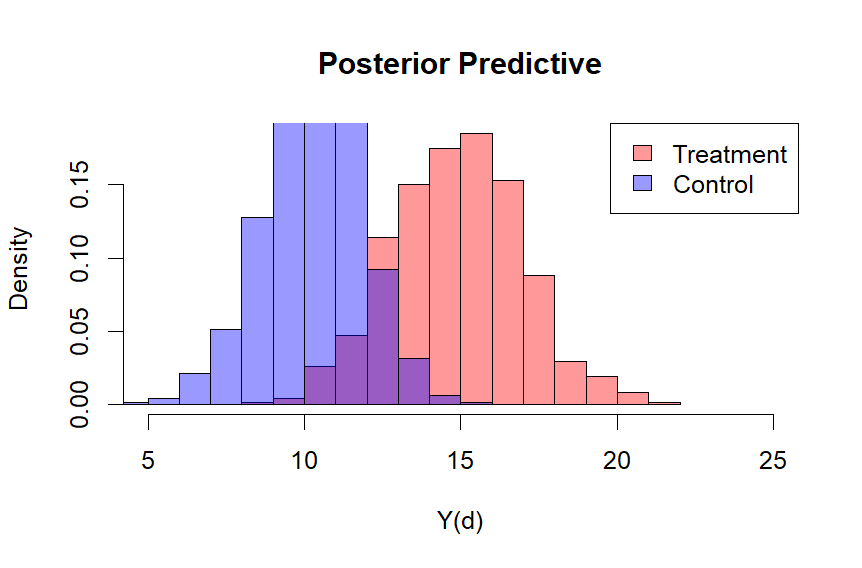
\includegraphics[width=340pt, height=200pt]{Chapters/chapter12/figures/BasicYd.png}
	\caption[List of figure caption goes here]{Predictive distributions: Potential outcomes.}\label{fig12_0}
\end{figure}


\begin{figure}
	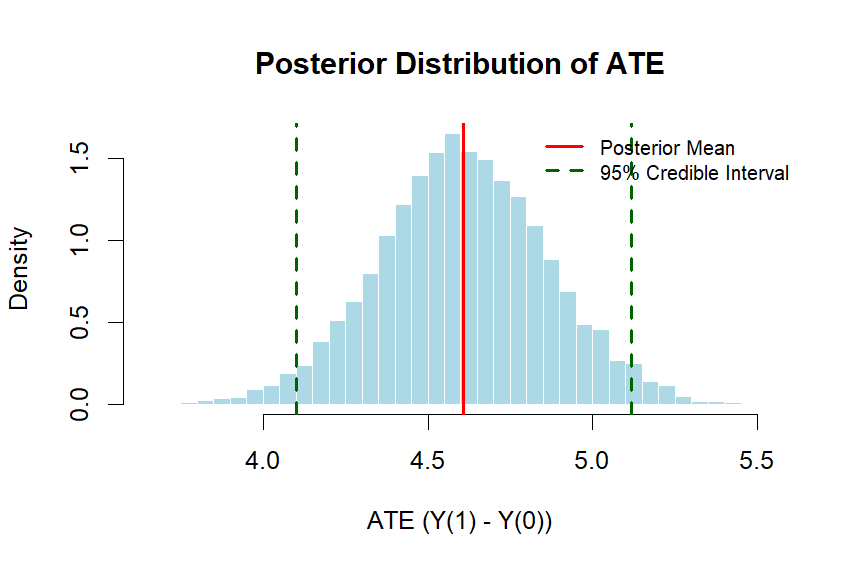
\includegraphics[width=340pt, height=200pt]{Chapters/chapter12/figures/BasicATE.png}
	\caption[List of figure caption goes here]{Posterior distribution: Average treatment effects.}\label{fig12_0a}
\end{figure}


An RCT is considered the gold standard for identifying causal effects because it provides the strongest basis for satisfying the key identification assumption in causal inference: \textit{independence between treatment assignment and potential outcomes}. However, RCTs may face challenges such as \textit{non-compliance}, which occurs when individuals do not adhere to their assigned treatment in an experimental study. This is important because, in many real-world settings, some individuals do not take the treatment they were assigned, leading to deviations from the ideal randomized controlled trial design. In addition, RCTs are sometimes infeasible due to ethical, logistical, or financial constraints. Moreover, they can be too narrowly focused or too localized to provide general conclusions about what works \cite{deaton2010instruments}. Thus, the \textit{external validity} of causal effects from RCTs may be questionable.  

It is also important to note that RCTs primarily identify the mean of the treatment effect distribution but do not capture other features, such as the median or higher-order moments. These additional aspects of the distribution of treatment effects can be highly relevant for policymakers and stakeholders. See \cite{deaton2010instruments} for a detailed discussion of other potential shortcomings of RCTs.


\section{Conditional independence assumption (CIA)}\label{chap12_3}

In practice, researchers often work with \textit{observational data}, where the treatment status is not randomly assigned because units actively choose the treatment they receive. In an RCT, the assignment mechanism is determined by chance, whereas in observational studies it is driven by choice. In these situations, we can identify the causal effect if the \textit{conditional independence assumption} (CIA) holds. This assumption states that the potential outcomes are independent of the treatment status, conditional on a set of observed  \textit{pre-treatment variables}:
\[
\{ Y_i(1), Y_i(0) \} \perp D_i \mid \mathbf{X}_i.
\]
This means that, conditional on the \textit{pre-treatment variables} $\mathbf{X}_i$, treatment assignment is as good as random. This property is known as \textit{unconfoundedness given} $\mathbf{X}_i$, or equivalently, the \textit{no unmeasured confounders} assumption. When this condition is combined with the requirement that, for all possible values of $\mathbf{X}_i$, there is a positive probability of receiving each treatment level ($0 < P(D_i = 1 \mid \mathbf{X}_i) < 1$), the joint condition is referred to as \textit{strong ignorability}. Identification of average causal effects in this setting also requires the SUTVA.

Note that under the CIA,
\begin{align*}
	\text{ATE} &= \mathbb{E}[Y_i(1)] - \mathbb{E}[Y_i(0)] \\
	&= \mathbb{E}_{\mathbf{X}}\left\{ \mathbb{E}[Y_i(1)\mid \mathbf{X}_i] - \mathbb{E}[Y_i(0)\mid \mathbf{X}_i] \right\} \\
	&= \mathbb{E}_{\mathbf{X}}\left\{ \mathbb{E}[Y_i(1)\mid \mathbf{X}_i, D_i=1] - \mathbb{E}[Y_i(0)\mid \mathbf{X}_i, D_i=0] \right\} \\
	&= \mathbb{E}_{\mathbf{X}}\left\{ \mathbb{E}[Y_i\mid \mathbf{X}_i, D_i=1] - \mathbb{E}[Y_i\mid \mathbf{X}_i, D_i=0] \right\} \\
	&= \mathbb{E}_{\mathbf{X}}\left\{ \tau(\mathbf{X}_i) \right\},
\end{align*}
where the second equality follows from the law of iterated expectations, the third uses CIA, and
\[
\tau(\mathbf{X}_i) = \mathbb{E}[Y_i \mid \mathbf{X}_i, D_i=1] - \mathbb{E}[Y_i \mid \mathbf{X}_i, D_i=0]
\]
is the \textit{conditional average treatment effect} (CATE) at covariate value $\mathbf{X}_i$, which captures treatment effect heterogeneity across different values of $\mathbf{X}$. Therefore, the ATE is the expectation of the CATE over the distribution of $\mathbf{X}$.

Figure~\ref{DAG2} illustrates the causal structure underlying the CIA. We follow the convention that time flows from left to right. Here, $\mathbf{X}$ -a vector of pre-treatment variables or \textit{confounders}- influences both the treatment ($D$) and the outcome ($Y$). Under the CIA, we can identify the causal effect of $D$ on $Y$ by adjusting for $\mathbf{X}$ because this causal structure satisfies the \textit{back-door criterion}. This criterion states that a set of variables $\mathbf{X}$ satisfies the condition for identifying the effect of $D$ on $Y$ if no variable in $\mathbf{X}$ is a descendant of $D$ and $\mathbf{X}$ blocks every back-door path from $D$ to $Y$. A \textit{back-door path} is any path from $D$ to $Y$ that begins with an arrow pointing into $D$. In Exercise~3, we ask to construct the DAG in Figure~\ref{DAG2}, verify that it is acyclic, and check whether the causal effect of \(D\) on \(Y\) is identifiable by controlling for \(\mathbf{X}\) using the package \textit{dagity}. In addition, Figure \ref{SWIG2} displays the SWIG. 

\begin{figure}[h!]
	\centering
	\begin{tikzpicture}[->,>=Stealth,shorten >=1pt,node distance=2.5cm,
		thick,main node/.style={circle,draw,minimum size=7mm}]
		\node[main node] (X) {$\mathbf{X}$};
		\node[main node] (D) [right of=X] {$D$};
		\node[main node] (Y) [right of=D] {$Y$};
		
		\path (X) edge (D)
		(X) edge[bend left=20] (Y)
		(D) edge (Y);
	\end{tikzpicture}
	\caption{Directed Acyclic Graph (DAG) implied by the Conditional Independence Assumption (CIA).}
	\label{DAG2}
\end{figure}

\begin{figure}[h!]
	\centering
	\begin{tikzpicture}[->,>=Stealth,shorten >=1pt,node distance=2.5cm,
		thick,main node/.style={circle,draw,minimum size=7mm}]
		% Nodes
		\node[main node] (X) {$\mathbf{X}$};
		\node[main node] (Dfix) [right of=X] {$D = d$}; % Intervention
		\node[main node] (Y) [right of=Dfix] {$Y(d)$};  % Counterfactual outcome
		\node[main node] (Dnat) [below of=Dfix, node distance=1.5cm] {$D$}; % Natural value
		
		% Edges
		\path (Dfix) edge[dashed] (Y)
		(X) edge[bend left=25] (Y)
		(X) edge (Dnat);
	\end{tikzpicture}
	\caption{Single-World Intervention Graph (SWIG) for $do(D=d)$: The treatment $D$ is split into the fixed intervention $D=d$ and its natural value. The outcome is replaced by $Y(d)$. $\mathbf{X}$ still influences $Y(d)$, so adjustment for $\mathbf{X}$ is needed for identification.}
	\label{SWIG2}
\end{figure}
 
The simple regression framework of the previous section can be extended to a multiple linear regression model by including the \textit{pre-treatment variables}; therefore, the CEF is linear in the treatment and pre-treatment variables:
\begin{align*}
	Y_i = \beta_0 + \tau D_i + \mathbf{X}_i^{\top}\boldsymbol{\beta} + \mu_i.
\end{align*}
Note that, by assumption in RCTs, $D_i$ and $\mathbf{X}_i$ are independent. Thus, the identification of $\tau$ is not affected under random assignment; however, including $\mathbf{X}_i$ helps explain part of the variability in $Y_i$, thereby improving the precision of the estimates.

On the other hand, if the CIA is satisfied, the error term in the linear regression is defined as
\[
\mu_i = Y_i(0) - \mathbb{E}[Y_i(0) \mid \mathbf{X}_i].
\]

Thus,
\[
\mathbb{E}[\mu_i \mid D_i, \mathbf{X}_i] = \mathbb{E}[Y_i(0) - \mathbb{E}[Y_i(0) \mid \mathbf{X}_i] \mid D_i, \mathbf{X}_i] 
= \mathbb{E}[Y_i(0) \mid D_i, \mathbf{X}_i] - \mathbb{E}[Y_i(0) \mid \mathbf{X}_i].
\]

By the CIA, $Y_i(0) \perp D_i \mid \mathbf{X}_i$, so:
\[
\mathbb{E}[Y_i(0) \mid D_i, \mathbf{X}_i] = \mathbb{E}[Y_i(0) \mid \mathbf{X}_i].
\]

Therefore:
\begin{equation}\label{eq:12_2}
	\mathbb{E}[\mu_i \mid D_i, \mathbf{X}_i] = 0.
\end{equation}

This condition is known as \textit{conditional mean independence}: after controlling for $\mathbf{X}_i$, treatment assignment is independent of unobserved determinants of the outcome. It justifies unbiased estimation of $\tau$ by regression adjustment in observational studies.\\

\textbf{Example: Treatment effect of 401(k) eligibility on net financial assets}

We study the average treatment effect of eligibility (\textit{e401}) for participation in the 401(k) retirement savings plan in the United States on net financial assets (\textit{net\_tfa}) using the dataset \textit{401k.csv}. The rationale for the exogeneity of 401(k) eligibility is that it becomes exogenous after conditioning on observable characteristics related to job choice, which may correlate with whether a firm offers this retirement plan \cite{chernozhukov2024applied}.

Accordingly, we control for the following covariates: age (\textit{age}), income (\textit{inc}), family size (\textit{fsize}), years of education (\textit{educ}), a marital status indicator (\textit{marr}), a two-earner status indicator (\textit{twoearn}), a defined benefit pension status indicator (\textit{db}), an IRA participation indicator (\textit{pira}), and a home ownership indicator (\textit{hown}). Under this specification, the key assumption is that eligibility is conditionally independent of net financial assets given these covariates \cite{chernozhukov2024applied}.

We can use the framework in Section \ref{sec61} to estimate the average treatment effect of 401k eligibility on net financial assets. The code \ref{code1_chap12} shows how to get the posterior distribution of this effect. Figure \ref{fig12_1} displays the posterior distribution of the treatment effect, the 95\% credible interval is (USD 3,473, USD 8,371), and the posterior mean is USD 5,903.

\begin{tcolorbox}[enhanced,width=4.67in,center upper,
	fontupper=\large\bfseries,drop shadow southwest,sharp corners]\label{code1_chap12}
	\textit{R code. Treatment effect: 401(k) eligibility on net financial assets}
	\begin{VF}
		\begin{lstlisting}[language=R]		
# 401k: Treatment effects
rm(list = ls())
set.seed(10101)

library(MCMCpack)
library(coda)
library(ggplot2)

mydata <- read.csv("https://raw.githubusercontent.com/BEsmarter-consultancy/BSTApp/refs/heads/master/DataApp/401k.csv", sep = ",", header = TRUE, quote = "")
attach(mydata )
y <- net_tfa 
# net_tfa: net financial assets
# Regressors quantity including intercept
X <- cbind(e401, age, inc, fsize, educ, marr, twoearn, db, pira, hown, 1)
# e401: 401k eligibility 
# age, income, family size, years of education, marital status indicator, two-earner status indicator, defined benefit pension status indicator, IRA participation indicator, and home ownership indicator.

# Posterior distributions using packages: MCMCpack sets the model in terms of the precision matrix. We use default parameters
posterior  <- MCMCpack::MCMCregress(y~X-1)
summary(coda::mcmc(posterior))

# Extract posterior samples for e401 (first coefficient)
beta_e401 <- posterior[, 1]

# Convert to data frame for ggplot
df_posterior <- data.frame(beta_e401)

# Plot with ggplot
ggplot(df_posterior, aes(x = beta_e401)) +
geom_density(fill = "steelblue", alpha = 0.6) +
geom_vline(xintercept = mean(beta_e401), color = "red", linetype = "dashed") +
labs(
title = "Posterior Distribution of Treatment Effect (e401)",
x = expression(beta[e401]),
y = "Density"
) +
theme_minimal(base_size = 14)
\end{lstlisting}
	\end{VF}
\end{tcolorbox}  

\begin{figure}
	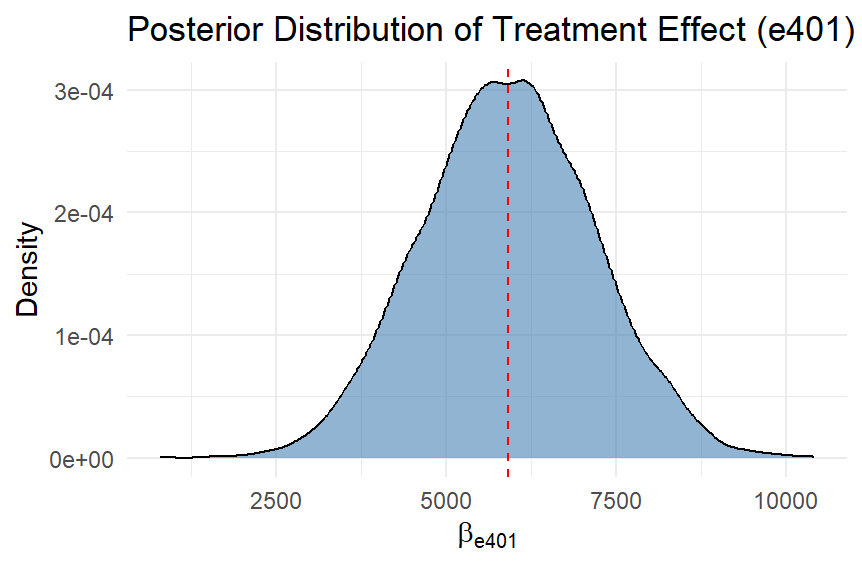
\includegraphics[width=340pt, height=200pt]{Chapters/chapter12/figures/TE401k.png}
	\caption[List of figure caption goes here]{Posterior distribution: Treatment effect 401k eligibility on net financial assets.}\label{fig12_1}
\end{figure}

Observe that the identification strategy relies on conditioning on $\mathbf{X}$. However, adding more controls is not always safe because some variables, known as \textit{bad controls}, can introduce bias if included in the adjustment set \cite{angrist2009mostly}. One important type of bad control is a \textit{collider}, a variable that is caused by (or is a common effect of) two or more other variables in a DAG. Colliders play a critical role because conditioning on them can create spurious associations between their causes, leading to what is known as \textit{collider bias} (or selection bias).

Figure~\ref{DAG3} illustrates this situation. Here, $C$ is a common effect of $D$ and $\mathbf{X}$. Conditioning on $C$ opens an additional path between $D$ and $Y$, creating a spurious association that violates the back-door criterion. In particular, the variable $C$ is a collider on the path $D \to C \leftarrow \mathbf{X}$. By default, a collider \textit{blocks} the flow of association along the path on which it lies, so this path is closed when $C$ is not conditioned on. However, conditioning on $C$ (or on any descendant of $C$) opens this path, creating a spurious association between $D$ and $\mathbf{X}$. Since $\mathbf{X}$ also affects $Y$, this induces bias in estimating the causal effect of $D$ on $Y$.\\ 

\begin{figure}[h]
	\centering
	\begin{tikzpicture}[->,>=Stealth,shorten >=1pt,node distance=2.5cm,
		thick,main node/.style={circle,draw,minimum size=7mm}]
		% Nodes
		\node[main node] (X) {$\mathbf{X}$};
		\node[main node] (D) [right of=X] {$D$};
		\node[main node] (Y) [right of=D] {$Y$};
		\node[main node] (C) [below of=Y, node distance=1cm] {$C$}; % Collider
		
		% Edges
		\path (X) edge (D)
		(X) edge[bend left=20] (Y)
		(D) edge (Y)
		(D) edge (C)
		(X) edge (C);
	\end{tikzpicture}
	\caption{Directed Acyclic Graph (DAG): The additional collider $C$ caused by both $D$ and $\mathbf{X}$ would open a path between $D$ and $\mathbf{X}$, inducing bias.}
	\label{DAG3}
\end{figure}

\textbf{Example: Birth-weight ``paradox", collider bias}

The collider bias illustrated in DAG \ref{fig:coll}, based on \cite{chernozhukov2024applied}, reflects the well-known Birth-weight ``paradox". This phenomenon arises when conditioning on an intermediate variable (birth weight, $B$) induces a spurious association between the binary indicator of smoking ($S$) and infant mortality ($Y$). In this setting, $U$ represents unobserved factors that affect both birth weight and infant mortality. Conditioning on $B$ creates collider bias because it opens a back-door path through the unobserved factors $U$ (dashed).

\begin{figure}[h!]
	\centering
	\begin{tikzpicture}[
		node distance=2cm,
		thick,
		main/.style={circle, draw, minimum size=8mm},
		>={Stealth}
		]
		
		% Nodes
		\node[main] (S) {$S$};
		\node[main] (B) [below right=1.2cm and 1.8cm of S] {$B$};
		\node[main, dashed] (U) [below left=1.2cm and 1.8cm of B] {$U$};
		\node[main] (Y) [right=1cm of B] {$Y$};
		
		% Arrows
		\draw[->] (S) -- (B);
		\draw[->] (S) -- (Y);
		\draw[->] (B) -- (Y);
		\draw[->] (U) -- (B);
		\draw[->] (U) -- (Y);
		
	\end{tikzpicture}
	\caption{DAG illustrating the birth-weight paradox: $S$ (smoking), $B$ (birth weight), $Y$ (infant mortality), $U$ (other unobserved health factors).}
	\label{fig:coll}
\end{figure}	

The code in \ref{code2_chap12} illustrates the bias by performing 100 replications, and Figure \ref{fig12_2} shows the distribution of posterior means across these replications. In this setting, the total effect of smoking on infant mortality is 2, consisting of a direct effect of 1 and an indirect effect through birth weight, also equal to 1.

\begin{tcolorbox}[enhanced,width=4.67in,center upper,
	fontupper=\large\bfseries,drop shadow southwest,sharp corners]\label{code2_chap12}
	\textit{R code. Collider bias: Birth weight ``paradox"}
	\begin{VF}
		\begin{lstlisting}[language=R]		
rm(list = ls()); set.seed(10101)
library(MCMCpack); library(dplyr); library(ggplot2)
# Parameters
n <- 1000; true_effect <- 2; replications <- 100
# Store results
results <- data.frame(rep = 1:replications, correct = numeric(replications), biased = numeric(replications))

for (r in 1:replications) {
	# Simulate data under DAG: S -> B -> Y, S -> Y, U -> B, U -> Y
	U <- rnorm(n, 0, 1); S <- rbinom(n, prob = 0.7, size = 1)
	B <- S + U + rnorm(n)
	Y <- S + B + 1.5*U + rnorm(n)
	# Correct model: does NOT condition on collider B
	model_correct <- MCMCregress(Y ~ S, burnin = 1000, mcmc = 3000, verbose = FALSE)
	# Biased model: conditions on collider B
	model_biased <- MCMCregress(Y ~ S + B, burnin = 1000, mcmc = 3000, verbose = FALSE)
	# Posterior means for S
	results$correct[r] <- mean(as.matrix(model_correct)[, "S"])
	results$biased[r] <- mean(as.matrix(model_biased)[, "S"])
}
# Compute bias
results <- results %>% mutate(
bias_correct = correct - true_effect,
bias_biased = biased - true_effect
)
# Average bias and SD
avg_bias <- results %>%
summarise(
mean_correct = mean(bias_correct),
mean_biased = mean(bias_biased),
sd_correct = sd(bias_correct),
sd_biased = sd(bias_biased)
)
print(avg_bias)
# Visualization: distribution of posterior means across 100 simulations
df_long <- results %>%
select(rep, correct, biased) %>%
tidyr::pivot_longer(cols = c(correct, biased), names_to = "model", values_to = "estimate")

ggplot(df_long, aes(x = estimate, fill = model)) + geom_density(alpha = 0.5) + geom_vline(xintercept = true_effect, color = "black", linetype = "dashed", linewidth = 1) + labs(title = "Posterior Means Across 100 Simulations", x = expression(paste("Posterior Mean of ", beta[S])), y = "Density") + theme_minimal(base_size = 14)
\end{lstlisting}
	\end{VF}
\end{tcolorbox}  

\begin{figure}[h!]
	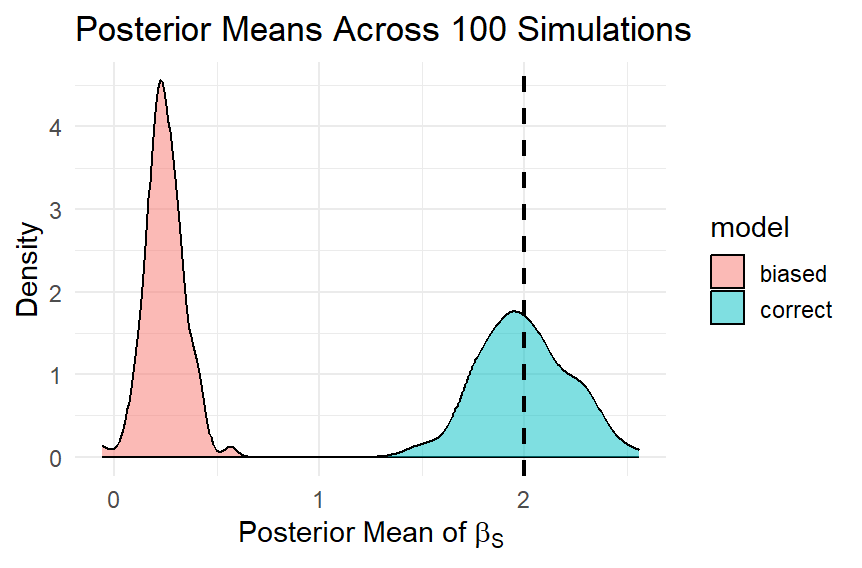
\includegraphics[width=340pt, height=200pt]{Chapters/chapter12/figures/FigColliderBias.png}
	\caption[List of figure caption goes here]{Posterior distribution: Posterior means of the collider bias example.}\label{fig12_2}
\end{figure}

Collider (selection) bias is one possible source of bias in the identification of causal effects. The well-known Heckman’s sample selection problem in econometrics \cite{heckman1979sample} can be interpreted as a form of collider bias because restricting the analysis to selected observations (e.g., those with positive wages) conditions on a variable that is a common effect of observed and unobserved factors, thereby opening a non-causal path and creating bias. In other words, the sample is no longer representative of the population, which undermines the identification of the causal effect. 

Other well-known sources of bias in econometrics include the omission of common causes affecting both the treatment and the outcome, that is, \textit{omission of correlated relevant regressors}, measurement error in regressors leading to \textit{attenuation bias} (where the estimated causal effect is biased toward zero), and \textit{simultaneous causality}, which often arises in systems of equations (see \cite{wooldridge2010econometric} for details). We will discuss these additional sources of bias later.

\section{Instrumental variables (IV)}\label{chap12_4}

In many real-world situations, we face biases such as those described in the previous paragraph, arising from measurement errors, omission of relevant variables, and similar issues. Even in these cases, it is still possible to identify the causal effect. One common strategy is to use a set of \textit{instrumental variables} ($\mathbf{Z}$) that satisfy two key conditions:
\begin{enumerate}
	\item \textit{Relevance}, meaning the instruments are correlated with the treatment:
	\[
	\mathbf{Z}_i \not\perp D_i.
	\]
	\item \textit{Exogeneity}, which in the linear model requires:
	\begin{equation}\label{eq:12_3}
		\mathbb{E}[\mu_i \mid \mathbf{Z}_i] = 0,
	\end{equation}
	and, in terms of potential outcomes, entails:
	\begin{itemize}
		\item \textit{Exclusion restriction}: instruments affect the outcome only through the treatment:
		\[
		Y_i(D_i = d, \mathbf{Z}_i = \mathbf{z}) = Y_i(D_i = d, \mathbf{Z}_i = \mathbf{z}') = Y_i(D_i = d), \quad d \in \{0,1\},
		\]
		\item \textit{Marginal exchangeability}: instruments are independent of the potential outcomes:
		\[
		\mathbf{Z}_i \perp \{ Y_i(1), Y_i(0) \}.
		\]
	\end{itemize}
\end{enumerate}

Relevance is testable, typically by checking whether instruments significantly predict the endogenous variable \cite{staiger1997instrumental,cragg1993testing,kleibergen2006generalized,stock2005asymptotic}. However, \textit{weak instruments}, those that exhibit only a weak association with the treatment, can lead to serious consequences, including a high level of uncertainty and the potential amplification of even small biases when estimating the causal effect.

Exogeneity is fundamentally untestable \cite{imbens1994identification}. However, when the number of instruments exceeds the number of endogenous variables, the Sargan test (or its robust version, the Hansen $J$-test) can be used to assess the validity of overidentifying restrictions. This test should not be misinterpreted as a direct test of the exclusion restriction. Instead, it evaluates whether the overidentifying restrictions implied by the IV model hold. Specifically, the null hypothesis states that all instruments are jointly uncorrelated with the structural error term, $\mathbb{E}[\mathbf{Z}^\top \mu] = \mathbf{0}$ \cite{sargan1958econometric,hansen1982large}. 

If the test rejects, it indicates that at least one instrument is invalid, but it does not reveal whether the violation arises from a failure of the exclusion restriction, correlation with unobserved confounders, or model misspecification. Conversely, if the test fails to reject, it only suggests that the sample moment conditions do not provide evidence against instrument validity under the maintained model. This outcome does not prove that the exclusion restrictions hold: the test may have low power, a mix of valid and invalid instruments could pass if violations ``cancel out'', and if the model is misspecified, a ``passing'' test is uninformative. 

In general, the exclusion restriction concerns unobservables (no correlation with the error term). Since the error term is not observed, the exclusion restriction can never be proven from the data; we can only look for evidence against it. Therefore, while the Sargan test is informative about overall instrument validity, it is not a separate or definitive test of the exclusion restriction \cite{wooldridge2010econometric,hayashi2000econometrics}.

Figure~\ref{DAG4} illustrates a situation where pre-treatment variables that influence both the treatment and the outcome are partially observed or measured with error. In such cases, an instrument can help identify the causal effect of the treatment on the outcome.

\begin{figure}[h]
	\centering
	\begin{tikzpicture}[->,>=Stealth,shorten >=1pt,node distance=2.5cm,
		thick,main node/.style={circle,draw,minimum size=7mm}]
		% Nodes
		\node[main node, dashed] (U) {$\mathbf{U}$};
		\node[main node] (D) [right of=X] {$D$};
		\node[main node] (Y) [right of=D] {$Y$};
		\node[main node] (Z) [below of=D, node distance=2cm] {$Z$};
		
		% Edges
		\path (Z) edge (D)
		(U) edge[bend left=20] (Y)
		(D) edge (Y)
		(U) edge (D);
	\end{tikzpicture}
	\caption{Directed Acyclic Graph (DAG) showing an instrumental variable $Z$ used to identify the causal effect of $D$ on $Y$ when some confounders $\mathbf{U}$ (dashed) are unobserved or measured with error.}
	\label{DAG4}
\end{figure}

However, the two conditions for instruments (relevance and exogeneity) only imply \textit{partial identification} of the Local Average Treatment Effect (LATE; see below, and \cite{Manski1989,manski1990nonparametric,manski1995identification,manski2003partial} for detailed treatments of partial identification). Thus, it is necessary to impose a third condition to achieve \textit{point identification} of a particular treatment effect using IV. This condition is \textit{monotonicity} which asserts that the instrument moves all units’ treatment decisions in the same direction, that is,
\[
D_i(1)\geq D_i(0), i=1,2,\dots,N,
\]
assuming a binary instrument $Z_i=\left\{0,1\right\}$. 

Note that monotonicity is also fundamentally untestable \cite{imbens1994identification}, as it refers to unobserved potential outcomes. However, its validity can be argued in the context of each application. We can examine whether the instrument shifts treatment in the expected direction. Moreover, if rich covariates are available, we can stratify by them and verify that, within each subgroup, the instrument increases (or at least does not decrease) the probability of treatment. For instance, we can analyze the cumulative distribution functions of the outcome when the binary instrumental variable takes values of 0 and 1; if the functions do not cross, this would suggest plausibility of the monotonicity assumption \cite{RamirezHassan2023}.

In the case where $Z_i$ denotes the assignment to treatment and $D_i$ the actual treatment status, there are four potential groups: \textit{always-takers} ($D = 1 \mid Z = 1$ and $D = 1 \mid Z = 0$), \textit{never-takers} ($D = 0 \mid Z = 1$ and $D = 0 \mid Z = 0$), \textit{compliers} ($D = 1 \mid Z = 1$ and $D = 0 \mid Z = 0$), and \textit{defiers} ($D = 0 \mid Z = 1$ and $D = 1 \mid Z = 0$). Note that these groups are not identified; for instance, we do not know whether an individual with $Z_i = 1$ and $D_i = 1$ is a complier or an always taker. The monotonicity assumption rules out defiers, meaning that the instrument (assignment to treatment) either does not change treatment status or only increases it.

Table \ref{tab:2x2} displays the distribution of unit types when defiers are ruled out by the monotonicity assumption. 

\begin{table}[ht]
	\centering
	\caption{Distribution of compliance types by instrument and treatment}\label{tab:2x2}
	\begin{tabular}{lcc}
		\hline
		& \multicolumn{2}{c}{\textbf{Treatment}} \\ 
		\cline{2-3}
		\textbf{Instrument} & $D_i = 0$ & $D_i = 1$ \\ 
		\hline
		$Z_i=0$  & Compliers, Never-takers & Always-takers \\[0.25em]
		$Z_i=1$  & Never-takers & Compliers, Always-takers \\ 
		\hline
	\end{tabular}
\end{table}

From this table we can identify the proportions of compliance types ($C$) as follows. The probability of always-takers (a) is
\[
P(C_i = a) = P(D_i=1 \mid Z_i=0),
\]
and the probability of never-takers (n) is
\[
P(C_i = n) = P(D_i=0 \mid Z_i=1).
\]
For compliers (c), note that
\[
P(D_i=1 \mid Z_i=1) = P(C_i=c) + P(C_i=a),
\]
so that
\[
P(C_i = c) = P(D_i=1 \mid Z_i=1) - P(D_i=1 \mid Z_i=0).
\]
Equivalently, using $D_i=0$,
\[
P(D_i=0 \mid Z_i=0) = P(C_i=n) + P(C_i=c),
\]
so that
\[
P(C_i = c) = P(D_i=0 \mid Z_i=0) - P(D_i=0 \mid Z_i=1).
\]

Therefore, under relevance, exogeneity, monotonicity, and SUTVA, IV methods allow identification of the causal effect for the subgroup of \textit{compliers}, that is, individuals who take the treatment when encouraged by the instrument and do not take it otherwise \cite{imbens1994identification,angrist1996identification}. This estimand is known as the \textit{Local Average Treatment Effect} (LATE) because it applies to a specific subpopulation rather than the entire population \cite{hernan2020causal}:

\begin{align*}
	\tau_{LATE} 
	&= \mathbb{E}[Y_i(1)-Y_i(0)\mid D_i(1)=1, D_i(0)=0].
\end{align*}

We define $Y_i(z_i,D_i(z))$ to be the outcome for unit $i$ if exposed to treatment $D_i(z)$ after being assigned to treatment $z$. Therefore, the \textit{Intention-to-Treat} (ITT) causal effect of $Z_i$ on $Y_i$ is:
{\scriptsize{
\begin{align*}
	\mathbb{E}[Y_i(1,D_i(1))-Y_i(0,D_i(0))]&=\underbrace{\mathbb{E}[Y_i(1,D_i(1))-Y_i(0,D_i(0))\mid D_i(1)=1,D_i(0)=1]\times P(D_i(1)=1,D_i(0)=1)}_{always-takers}\\
	&+\underbrace{\mathbb{E}[Y_i(1,D_i(1))-Y_i(0,D_i(0))\mid D_i(1)=0,D_i(0)=0]\times P(D_i(1)=0,D_i(0)=0)}_{never-takers}\\
	&+\underbrace{\mathbb{E}[Y_i(1,D_i(1))-Y_i(0,D_i(0))\mid D_i(1)=1,D_i(0)=0]\times P(D_i(1)=1,D_i(0)=0)}_{compliers}\\
	&+\underbrace{\mathbb{E}[Y_i(1,D_i(1))-Y_i(0,D_i(0))\mid D_i(1)=0,D_i(0)=1]\times P(D_i(1)=0,D_i(0)=1)}_{defiers},\\
\end{align*}
}}
that is, ITT is a mixture over the four potential groups.

We know that the ITT effect of $Z_i$ on $Y_i$ is zero for always-takers and never-takers due to the exclusion restriction, i.e., $Z_i$ affects $Y_i$ only through $D_i$, and $D_i$ does not vary with $Z_i$ for always-takers and never-takers. Moreover, the monotonicity assumption rules out the existence of defiers. Hence, only compliers contribute to the effect of $Z_i$ on $Y_i$:

{\scriptsize
	\begin{align*}
		\mathbb{E}[Y_i(1,D_i(1)) - Y_i(0,D_i(0))] 
		&= \mathbb{E}[Y_i(1,D_i(1)) - Y_i(0,D_i(0)) \mid D_i(1)=1, D_i(0)=0] \cdot P(D_i(1)=1, D_i(0)=0).
	\end{align*}
}

For compliers, $D_i = Z_i$, so we can simplify $Y_i(1,D_i(1)) = Y_i(1,1) = Y_i(1)$ and $Y_i(0,D_i(0)) = Y_i(0,0) = Y_i(0)$. Thus,

\begin{align*}
	\mathbb{E}[Y_i(1) - Y_i(0)] 
	&= \mathbb{E}[Y_i(1) - Y_i(0) \mid D_i(1) = 1, D_i(0) = 0] \cdot P(D_i(1) = 1, D_i(0) = 0),
\end{align*}

which implies that

\begin{align*}
	\tau_{LATE} = \mathbb{E}[Y_i(1) - Y_i(0) \mid D_i(1) = 1, D_i(0) = 0] 
	&= \frac{\mathbb{E}[Y_i(1) - Y_i(0)]}{P(D_i(1) = 1, D_i(0) = 0)}.
\end{align*}

Under the assumption that the instrument \( Z_i \) is independent of the potential outcomes (i.e., marginal exchangeability), we have
\[
\tau_{LATE} = \mathbb{E}[Y_i(1) - Y_i(0) \mid D_i(1) = 1, D_i(0) = 0] 
= \frac{\mathbb{E}[Y_i \mid Z_i = 1] - \mathbb{E}[Y_i \mid Z_i = 0]}{P(D_i(1) = 1, D_i(0) = 0)}.
\]

We know that $P(D_i(1) = 1, D_i(0) = 0)=P(D_i = 1 \mid Z_i = 1) - P(D_i = 1 \mid Z_i = 0)$, and taking into account that \( \mathbb{E}[D_i \mid Z_i] = P(D_i = 1 \mid Z_i) \), we obtain
\[
\tau_{LATE} = \frac{\mathbb{E}[Y_i \mid Z_i = 1] - \mathbb{E}[Y_i \mid Z_i = 0]}{\mathbb{E}[D_i \mid Z_i = 1] - \mathbb{E}[D_i \mid Z_i = 0]}.
\]

This is the standard instrumental variables (IV) estimand, often referred to as the \textit{Wald estimator}. Note that the \textit{relevance condition} is required to ensure identification, i.e.,
\[
\mathbb{E}[D_i \mid Z_i = 1] - \mathbb{E}[D_i \mid Z_i = 0] \neq 0,
\]
that is, the instrument is strong enough that some units actually comply, this means, there is a proportion of compliers in the population.

The IV estimand represents the ratio of the intention-to-treat effect on the outcome to the intention-to-treat effect on the treatment (i.e., the proportion of compliers). The instrument induces random variation in treatment: the numerator captures how outcomes respond to the instrument, and the denominator captures how treatment responds to the instrument. Dividing the two isolates the causal effect for compliers.

Note that the LATE is not the global average causal effect, and has been subject to several criticisms. First, the proportion of compliers in the population may be small, raising concerns about the policy relevance of this estimand. Observe that while we cannot identify all four principal strata (compliers, never-takers, always-takers, and defiers), the proportion of compliers is identifiable. Second, the monotonicity assumption is not always plausible, particularly in observational studies where instruments may induce heterogeneous behavioral responses. Third, partitioning the population into four strata can become ill-defined in settings where instruments arise from different mechanisms or individual-specific criteria \cite{deaton2010instruments,hernan2020causal}. For arguments in defense of LATE against these critiques, see \cite{angrist2010better}.\\

\textbf{Example: A simple setting for point and set identified LATE}

Assume that we see the results display in Table \ref{tab:types}.

\begin{table}[ht]
	\centering
	\caption{Distribution of units by type, instrument, treatment, and outcomes}
	\label{tab:types}
	\begin{tabular}{lcccc}
		\hline
		Type & $Z_{obs}$ & $D_{obs}$ & $Y_{obs}$ & Units \\
		\hline
		Compliers, Never-takers & 0 & 0 & 3 & 50 \\
		Never-takers   & 1 & 0 & 4 & 20  \\
		Compliers, Always-takers & 1 & 1 & 7 & 100  \\
		 Always-takers   & 0 & 1 & 5 & 30  \\
		\hline
	\end{tabular}
\end{table}

Let's calculate the LATE assuming exclusion restrictions, and without assuming exclusion restrictions.

We first estimate the \textit{first stage and reduced form.}

\[
E[D \mid Z=0] = \tfrac{30}{80} = 0.37, \quad
E[D \mid Z=1] = \tfrac{100}{120} = 0.83,
\]
\[
\Delta_D = E[D \mid Z=1] - E[D \mid Z=0] = 0.46.
\]

\[
E[Y \mid Z=0] = \tfrac{3 \cdot 50 + 5 \cdot 30}{80} = 3.75, \quad
E[Y \mid Z=1] = \tfrac{4 \cdot 20 + 7 \cdot 100}{120} = 6.50,
\]
\[
\Delta_Y = E[Y \mid Z=1] - E[Y \mid Z=0] = 2.75.
\]

From these we also recover the compliance shares:
\[
\eta_a = P(D=1 \mid Z=0) = \tfrac{3}{8}=0.375, \quad
\eta_c = \Delta_D = \tfrac{11}{24}=0.458,
\]
thus,
\[
\eta_n = 1 - \eta_a - \eta_c = \tfrac{1}{6}=0.166.
\]

Then, we can \textit{point-identified} the LATE under exclusion restriction,

\[
\text{LATE} = \frac{\Delta_Y}{\Delta_D}
= \frac{2.75}{0.46}
= 6.
\]

We achieved point identification by imposing the exclusion restriction, which requires that treatment assignment is unrelated to potential outcomes for never-takers and always-takers.\footnote{Note that under monotonicity, defiers are ruled out, whereas for compliers, the exclusion restriction is not a separate assumption: by construction, their potential outcomes are indexed only by treatment status, since the instrument deterministically shifts them between $D_i=0$ and $D_i=1$. Thus, the exclusion restriction applies only to never-takers and always-takers, whose treatment status does not vary with the instrument.} This, is
\[
E[Y \mid Z=1, C=n] = E[Y \mid Z=0, C=n],
\]
and
\[
E[Y \mid Z=1, C=a] = E[Y \mid Z=0, C=a].
\]
Without exclusion restrictions, we should take into account that 

\[
\delta_n = E[Y \mid Z=1, C=n] - E[Y \mid Z=0, C=n] \neq 0,
\]
\[
\delta_a = E[Y \mid Z=1, C=a] - E[Y \mid Z=0, C=a] \neq 0.
\]

Then
\[
\Delta_Y = \eta_c \cdot \text{LATE} + \eta_n \delta_n + \eta_a \delta_a,
\]
Thus,
\[
\text{LATE} = \frac{\Delta_Y - \eta_n \delta_n - \eta_a \delta_a}{\eta_c}.
\]

From the table we know
\[
E[Y \mid Z=1, C=n] = 4, \quad E[Y \mid Z=0, C=a] = 5.
\]

We assume that the bounding outcomes come from the observed support \(Y \in [3,7]\). Then,
\[
\delta_n \in [-3,1], \quad \delta_a \in [-2,2].
\]

Therefore,
\[
\text{LATE}_{\min} = \frac{\Delta_Y - \eta_n \cdot 1 - \eta_a \cdot 2}{\eta_c}
= 4,
\]

\[
\text{LATE}_{\max} = \frac{\Delta_Y - \eta_n (-3) - \eta_a (-2)}{\eta_c}
= 8.73.
\]

Then, without exclusion restrictions the LATE is \textit{set identified}, \(\text{LATE} \in [4, 8.73]\), and with exclusion restrictions, LATE is \textit{point identified}, \(\text{LATE} = 6\).\\

\textbf{Example: Effects of vitamin A supplements on children's survival}

This example is taken from \cite{imbens1997bayesian}. The authors perform Bayesian inference for causal effects in a completely randomized experiment with no covariates and partial compliance. The experiment was conducted in Indonesia, where children were randomly assigned to receive vitamin A supplements. No individual assigned to the control group ($Z_i = 0$) actually took the vitamin, meaning that $D_i(0) = 1$ was never observed. This rules out always-takers and defiers. However, some individuals assigned to the treatment group ($Z_i = 1$) did not take the vitamin, so $D_i(1) = 0$ occurred for some units. Consequently, $D_i(1) \geq D_i(0)$ holds for all individuals (there are not defiers), satisfying the monotonicity assumption. Under this setting, the population consists only of compliers and never-takers.

\begin{table}[h!]
	%\centering % This ensures the table is centered on the page
	\caption{Effects of vitamin A supplements on children's survival \cite{imbens1997bayesian}}
	\label{tab:observed_data}
	\begin{minipage}{0.5\textwidth}
		%\centering % Centers the content inside minipage
		\begin{tabular}{lcccr}
			\hline
			\multirow{2}{*}{\textbf{Type}} & \textbf{Assignment} & \textbf{Treatment} & \textbf{Survival}  & \textbf{Units} \\
			& $Z_{\text{obs},i}$ & $D_{\text{obs},i}$ & $Y_{\text{obs},i}$ & 23,682 \\
			\hline
			Complier or never-taker & 0 & 0 & 0 & 74 \\
			Complier or never-taker & 0 & 0 & 1 & 11,514 \\
			Never-taker & 1 & 0 & 0 & 34 \\
			Never-taker & 1 & 0 & 1 & 2,385 \\
			Complier & 1 & 1 & 0 & 12 \\
			Complier & 1 & 1 & 1 & 9,663 \\
			\hline
		\end{tabular}
	\end{minipage}
\end{table}

Table \ref{tab:observed_data} summarizes the data. Using this table, we can illustrate key concepts in the identification of causal effects with noncompliance. Let $C_i$ denote the compliance type of individual $i$, which in this case can be either a complier ($c$) or a never-taker ($n$). The probability of being a complier, $\omega := P(C_i = c)$, is given by
\begin{align*}
	P(C_i = c) 
	&= \underbrace{P(D_i = 1 \mid Z_i = 1)}_{P(\text{compliers}) + P(\text{always-takers})} 
	- \underbrace{P(D_i = 1 \mid Z_i = 0)}_{P(\text{always-takers}) = 0} \\
	&= \frac{P(D_i = 1, Z_i = 1)}{P(Z_i = 1)}.
\end{align*}
Thus, the ML estimate is
\[
\hat{\omega} = \frac{12 + 9{,}663}{12 + 9{,}663 + 34 + 2{,}385}= 0.8.
\]
Note that $P(C_i = n) = 1 - P(C_i = c)$ in this example; thus, the ML estimate is $1-\hat{\omega} = 0.2$.

The probability of survival for compliers assigned to treatment, $\eta_{c1} := P(Y_i = 1 \mid C_i = c, Z_i = 1)$, is
\begin{align*}
	P(Y_i = 1 \mid C_i = c, Z_i = 1) 
	&= \frac{P(Y_i = 1, C_i = c \mid Z_i = 1) \times P(Z_i = 1)}{P(C_i = c \mid Z_i = 1) \times P(Z_i = 1)}.
\end{align*}
Thus, the ML estimate is $\hat{\eta}_{c1}= \frac{9{,}663}{9{,}663 + 12}= 0.999.$

Similarly, the probability of survival for never-takers assigned to treatment, $\eta_{n1} := P(Y_i = 1 \mid C_i = n, Z_i = 1)$, is
\begin{align*}
	P(Y_i = 1 \mid C_i = n, Z_i = 1) 
	&= \frac{P(Y_i = 1, C_i = n \mid Z_i = 1) \times P(Z_i = 1)}{P(C_i = n \mid Z_i = 1) \times P(Z_i = 1)}.
\end{align*}
Consequently, the ML estimate is $\hat{\eta}_{n1} = \frac{2{,}385}{2{,}385 + 34} = 0.986.$

Note that $\eta_{c0} = P(Y_i = 1 \mid C_i = c, Z_i = 0)$ and $\eta_{n0} = P(Y_i = 1 \mid C_i = n, Z_i = 0)$ cannot be \textit{point-identified}. However, we can obtain \emph{set identification} because
\begin{align*}
	\eta_0:=P(Y_i = 1 \mid Z_i = 0) 
	&= P(Y_i = 1 \mid Z_i = 0, C_i = c) \times P(C_i = c) \\
	&\quad + P(Y_i = 1 \mid Z_i = 0, C_i = n) \times P(C_i = n) \\
	&= \frac{P(Y_i = 1, Z_i = 0)}{P(Z_i = 0)},
\end{align*} where the ML estimate is $\hat{\eta}_0= \frac{11{,}514}{11{,}514 + 74}= 0.9936.$

The first equality holds because the probability of survival given no treatment assignment is expressed as a mixture by the law of total probability, and the second equality follows from Bayes' rule.

This implies that 
\[
0.9936 = \hat{\omega} \hat{\eta}_{c0} + (1-\hat{\omega})\hat{\eta}_{n0},
\]
which leads to 
\[
\hat{\eta}_{n0} = 4.968 - 4\hat{\eta}_{c0}.
\]
Given that probabilities must lie in the unit interval, such that $0 \leq 4.968 - 4\hat{\eta}_{c0} \leq 1$, we obtain:  
(i) $\hat{\eta}_{c0} \leq 1 \leq 1.242$ (automatically satisfied), and  
(ii) $4\hat{\eta}_{c0} \geq 4.968 - 1 = 3.968$, which implies $\hat{\eta}_{c0} \geq 0.992$.  

Consequently, the ML estimates $\hat{\eta}_{c0} \in [0.992, 1]$ and $\hat{\eta}_{n0} \in [0.968, 1]$.

These results imply that the \textit{complier average causal effect} (CACE) is
\begin{align*}
	\tau_{CACE} &= \mathbb{E}[Y_i(1)-Y_i(0)\mid D_i(1)=1,D_i(0)=0] \\
	&= P[Y_i = 1 \mid C_i = c, Z_i = 1] - P[Y_i = 1 \mid C_i = c, Z_i = 0] \\
	&= \eta_{c1} - \eta_{c0},
\end{align*}
where the first line is the formal definition, the second equality uses random assignment to express the estimand in terms of observed probabilities, and the third relies on the model parameterization.

The CACE is only set-identified, yielding the interval
\[
\hat{\tau}_{CACE} \in [-0.001, 0.007],
\]
meaning that the survival rate among compliers can vary between -1 and 7 per 1,000 children due to vitamin A supplementation.

Remember that point identification can be achieved by imposing the exclusion restriction, which requires that treatment assignment is unrelated to potential outcomes for never-takers and always-takers. Under this assumption,
\[
P(Y_i = y \mid C_i = n, Z_i = z) = P(Y_i = y \mid C_i = n),
\]
so that $\hat{\eta}_{n1} = \hat{\eta}_{n0} = \hat{\eta}_n = 0.986$. Substituting into the mixture equation yields $\hat{\eta}_{c0} = 0.9955$, and consequently,
\[
\hat{\tau}_{CACE} = 0.0035,
\]
indicating that survival increases by approximately 3.5 per 1,000 children due to vitamin A supplementation.\footnote{CACE and LATE refer to the same estimand -the average causal effect for compliers- under monotonicity and the exclusion restriction. If the exclusion restriction fails, they differ because LATE (as identified by IV) no longer equals the complier-specific causal effect (CACE).}
 
We use conjugate families to perform Bayesian inference in this example. Specifically, we adopt the Bernoulli-Beta model (see Section \ref{sec42}) with independent non-informative Beta priors, each having parameters equal to 1. This corresponds to a uniform distribution on the interval $(0,1)$.  

An advantage of the Bayesian formulation is that, after applying data augmentation with the compliance type $C_i$, all the conditional posterior distributions are Beta (See \cite{imbens1997bayesian} for details in derivations). In particular:
\[
\omega \mid \mathbf{C}, \mathbf{Z}_{\text{obs}}, \mathbf{D}_{\text{obs}}, \mathbf{Y}_{\text{obs}} \sim \text{Beta}(1 + N_c,\, 1 + N_n),
\]
where $N_c$ and $N_n$ denote the number of compliers and never-takers, respectively.
\[
\eta_{c1} \mid \mathbf{C}, \mathbf{Z}_{\text{obs}}, \mathbf{D}_{\text{obs}}, \mathbf{Y}_{\text{obs}} \sim \text{Beta}(1 + 9{,}663,\, 1 + 12),
\]
\[
\eta_{n1} \mid \mathbf{C}, \mathbf{Z}_{\text{obs}}, \mathbf{D}_{\text{obs}}, \mathbf{Y}_{\text{obs}} \sim \text{Beta}(1 + 2{,}385,\, 1 + 34),
\]
\[
\eta_{c0} \mid \mathbf{C}, \mathbf{Z}_{\text{obs}}, \mathbf{D}_{\text{obs}}, \mathbf{Y}_{\text{obs}} \sim \text{Beta}(1 + N_{c01},\, 1 + N_{c00}),
\]
where $N_{c01}$ and $N_{c00}$ are the numbers of compliers in the control group who survived and did not survive, respectively.
\[
\eta_{n0} \mid \mathbf{C}, \mathbf{Z}_{\text{obs}}, \mathbf{D}_{\text{obs}}, \mathbf{Y}_{\text{obs}} \sim \text{Beta}(1 + N_{n01},\, 1 + N_{n00}),
\]
where $N_{n01}$ and $N_{n00}$ are the numbers of never-takers in the control group who survived and did not survive, respectively.

In addition, the conditional probability of being a complier is given by:
\[
P(C_i = c \mid Z_{\text{obs},i}, D_{\text{obs},i}, Y_{\text{obs},i}) =
\begin{cases}
	0, & i \in \{Z_i = 1, D_i = 0\},\\
	1, & i \in \{Z_i = 1, D_i = 1\},\\
	\dfrac{\omega g_{c0,i}}{\omega g_{c0,i} + (1-\omega) g_{n0,i}}, & i \in \{Z_i = 0\},
\end{cases}
\]
where $g_{c0,i} = \eta_{c0}^{Y_{\text{obs},i}} (1 - \eta_{c0})^{1 - Y_{\text{obs},i}}$ and $g_{n0,i} = \eta_{n0}^{Y_{\text{obs},i}} (1 - \eta_{n0})^{1 - Y_{\text{obs},i}}$. Note that $Y_{\text{obs},i} = 1$ implies $g_{c0,i} = \eta_{c0}$ and $g_{n0,i} = \eta_{n0}$, while $Y_{\text{obs},i} = 0$ implies $g_{c0,i} = (1 - \eta_{c0})$ and $g_{n0,i} = (1 - \eta_{n0})$.

The following code shows the implementation, and the corresponding figure displays the posterior distribution of the CACE, the mean is 0.0024, and the 95\% credible intervals is (-0.0012, 0.0071).

\begin{tcolorbox}[enhanced,width=4.67in,center upper,
	fontupper=\large\bfseries,drop shadow southwest,sharp corners]\label{codea_chap12}
	\textit{R code. Effects of vitamin A supplements on children's survival}
	\begin{VF}
		\begin{lstlisting}[language=R]
rm(list = ls()); set.seed(10101)
library(dplyr)
# Simulate data
Nc111 <- 9663
c111 <- cbind(rep(1, Nc111), rep(1, Nc111), rep(1, Nc111)) 
Nc110 <- 12
c110 <- cbind(rep(1, Nc110), rep(1, Nc110), rep(0, Nc110)) 
Nn101 <- 2385
n101 <- cbind(rep(1, Nn101), rep(0, Nn101), rep(1, Nn101)) 
Nn100 <- 34
n100 <- cbind(rep(1, Nn100), rep(0, Nn100), rep(0, Nn100)) 
Ncn001 <- 11514
cn001 <- cbind(rep(0, Ncn001), rep(0, Ncn001), rep(1, Ncn001)) 
Ncn000 <- 74
cn000 <- cbind(rep(0, Ncn000), rep(0, Ncn000), rep(0, Ncn000)) 

mydata <- rbind(c111, c110, n101, n100, cn001, cn000)
mydata <- data.frame(Z = mydata[,1], D = mydata[,2], Y = mydata[,3])
N <- dim(mydata)[1]
attach(mydata)

# Sampling function C (type)
SampleType <- function(z, d, y, wc, nc0, nn0){
	if(z == 1 & d == 0){
		pc <- 0
	}else{
		if(z == 1 & d == 1){
			pc <- 1
		}else{
			if(y == 1){
				pc <- (wc * nc0) / (wc * nc0 +  (1 - wc) * nn0)
			}else{
				pc <- (wc * (1 - nc0)) / (wc * (1 - nc0) +  (1 - wc) * (1 - nn0))
			}
		}
	}
	rbinom(1, 1, prob = pc) # 1: Complier/ 0: Never taker
}
z = 0; d = 0; y = 0; wc = 0.8; nc0 = 0.9; nn0 = 0.05
SampleType(z = z, d = d, y = y, wc = wc, nc0 = nc0, nn0 = nn0)
Clat <- sapply(1:N, function(i){SampleType(z = Z[i], d = D[i], y = Y[i], wc = wc, nc0 = nc0, nn0 = nn0)})
\end{lstlisting}
	\end{VF}
\end{tcolorbox} 


\begin{tcolorbox}[enhanced,width=4.67in,center upper,
	fontupper=\large\bfseries,drop shadow southwest,sharp corners]
	\textit{R code. Effects of vitamin A supplements on children's survival}
	\begin{VF}
		\begin{lstlisting}[language=R]
# Gibbs sampler
a0 <- 1; b0 <- 1 # Hyperparameters beta priors
burnin <- 500; S <- 2000; tot <- S + burnin 
PosteriorDraws <- matrix(NA, tot, 5)
pb <- txtProgressBar(min = 0, max = tot, style = 3)

for(s in 1:tot){
	dataLat <- cbind(mydata, Clat)
	Nc011 <- sum(dataLat$Z == 0 & dataLat$Clat == 1 & dataLat$Y == 1)
	Nc010 <- sum(dataLat$Z == 0 & dataLat$Clat == 1 & dataLat$Y == 0)
	Nn001 <- sum(dataLat$Z == 0 & dataLat$Clat == 0 & dataLat$Y == 1)
	Nn000 <- sum(dataLat$Z == 0 & dataLat$Clat == 0 & dataLat$Y == 0)
	Nc <- sum(Clat == 1)
	Nn <- sum(Clat == 0)
	wc <- rbeta(1, 1 + Nc, 1 + Nn)
	nc1 <- rbeta(1, 1 + Nc111, 1 + Nc110)
	nn1 <- rbeta(1, 1 + Nn101, 1 + Nn100)
	nc0 <- rbeta(1, 1 + Nc011, 1 + Nc010)
	nn0 <- rbeta(1, 1 + Nn001, 1 + Nn000)
	Clat <- sapply(1:N, function(i){SampleType(z = Z[i], d = D[i], y = Y[i], wc = wc, nc0 = nc0, nn0 = nn0)})
	PosteriorDraws[s, ] <- c(wc, nc1, nc0, nn1, nn0)
	setTxtProgressBar(pb, s)
}
close(pb)
keep <- seq((burnin+1), tot)
LATE <- PosteriorDraws[keep, 2] - PosteriorDraws[keep, 3]
LATEmean <- mean(LATE)
LATEci <- quantile(LATE, c(0.025, 0.975))

# Plot posterior distribution of CATE
hist(LATE, breaks = 40, freq = FALSE,
main = "Posterior Distribution of CACE",
xlab = "CACE", col = "lightblue", border = "white")
abline(v = LATEmean, col = "red", lwd = 2)
abline(v = LATEci, col = "darkgreen", lty = 2, lwd = 2)

legend("topright", legend = c("Posterior Mean", "95% Credible Interval"),
col = c("red", "darkgreen"), lwd = 2, lty = c(1, 2),
bty = "n", cex = 0.8)  # Smaller legend using cex
\end{lstlisting}
	\end{VF}
\end{tcolorbox} 

\begin{figure}[h!]
	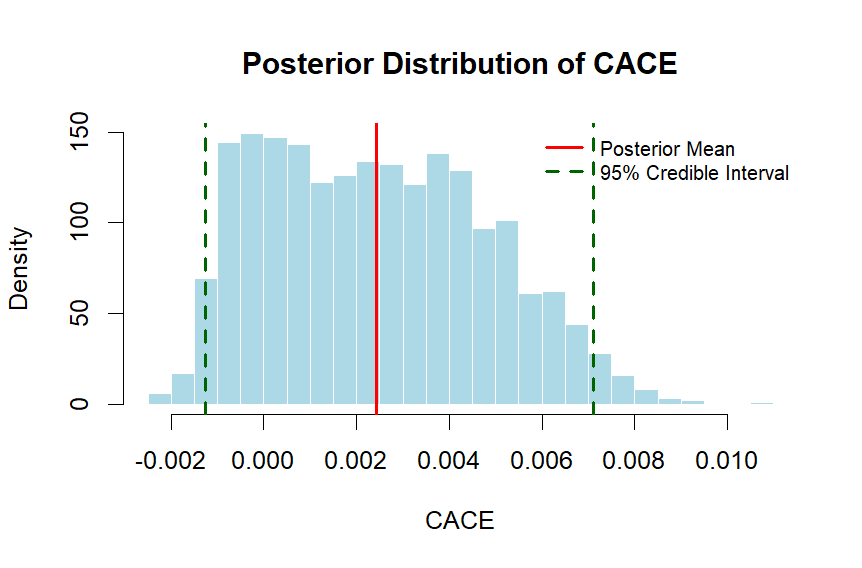
\includegraphics[width=340pt, height=200pt]{Chapters/chapter12/figures/CACE.png}
	\caption[List of figure caption goes here]{Posterior distribution: Complier average causal effect of vitamin A supplements.}\label{fig12_CACE}
\end{figure}

We can perform inference by imposing the exclusion restriction, setting $\eta_{n} = \eta_{n0} = \eta_{n1}$, so that the posterior distribution is
\[
\eta_{n} \mid \mathbf{C}, \mathbf{Z}_{\text{obs}}, \mathbf{D}_{\text{obs}}, \mathbf{Y}_{\text{obs}} \sim \text{Beta}(1 + N_{n1},\, 1 + N_{n0}),
\]
where $N_{n1}$ and $N_{n0}$ denote the numbers of never-takers who survived and did not survive, respectively. This is the only modification to the Gibbs sampler.  

The following code shows the implementation, and Figure~\ref{fig12_LATE} displays the posterior distribution of the CACE (which equals the LATE under the exclusion restriction). The posterior mean is 0.0030, and the 95\% credible interval is (0.0008, 0.0054). Therefore, imposing the exclusion restriction leaves the posterior mean approximately unchanged but increases the precision and informativeness of the posterior distribution. Without the restriction, the posterior was relatively flat within the 95\% credible interval, whereas under the exclusion restriction, the posterior distribution is approximately normal, resulting in a narrower 95\% credible interval.

Thus, this example illustrates how the Bayesian framework provides a way to quantify uncertainty and conduct sensitivity analysis regarding the exclusion restriction. See \cite{hirano2000assessing} for an extension controlling for covariates. 

In addition, it is worth mentioning that in partially identified models, the asymptotic equivalence between Bayesian and Frequentist inference breaks down. In particular, credible sets for partially identified parameters tend to be smaller than confidence sets asymptotically \cite{MoonSchorfheide2012}. This occurs because the posterior remains asymptotically sensitive to the prior, and Bayesian credible sets lie strictly inside the true identified set. To address this disagreement, \cite{Giacomini2021} propose a multi-prior robust Bayesian approach that helps reconcile Bayesian and Frequentist inference in set-identified models, which are a special case of partially identified models.

\begin{tcolorbox}[enhanced,width=4.67in,center upper,
	fontupper=\large\bfseries,drop shadow southwest,sharp corners]
	\textit{R code. Effects of vitamin A supplements on children's survival}
	\begin{VF}
		\begin{lstlisting}[language=R]
PosteriorDrawsER <- matrix(NA, tot, 4)
pb <- txtProgressBar(min = 0, max = tot, style = 3)

for(s in 1:tot){
	dataLat <- cbind(mydata, Clat)
	Nc011 <- sum(dataLat$Z == 0 & dataLat$Clat == 1 & dataLat$Y == 1)
	Nc010 <- sum(dataLat$Z == 0 & dataLat$Clat == 1 & dataLat$Y == 0)
	Nn01 <- sum(dataLat$Clat == 0 & dataLat$Y == 1)
	Nn00 <- sum(dataLat$Clat == 0 & dataLat$Y == 0)
	Nc <- sum(Clat == 1)
	Nn <- sum(Clat == 0)
	wc <- rbeta(1, 1 + Nc, 1 + Nn)
	nc1 <- rbeta(1, 1 + Nc111, 1 + Nc110)
	nn <- rbeta(1, 1 + Nn01, 1 + Nn00)
	nc0 <- rbeta(1, 1 + Nc011, 1 + Nc010)
	Clat <- sapply(1:N, function(i){SampleType(z = Z[i], d = D[i], y = Y[i], wc = wc, nc0 = nc0, nn0 = nn)})
	PosteriorDrawsER[s, ] <- c(wc, nc1, nc0, nn)
	setTxtProgressBar(pb, s)
}
close(pb)
keep <- seq((burnin+1), tot)
LATEER <- PosteriorDrawsER[keep, 2] - PosteriorDrawsER[keep, 3]
LATEERmean <- mean(LATEER)
LATEERci <- quantile(LATEER, c(0.025, 0.975))
# Plot posterior distribution of ATE
hist(LATE, breaks = 40, freq = FALSE,
main = "Posterior Distribution of CACE",
xlab = "CACE", col = "lightblue", border = "white")
abline(v = LATEmean, col = "red", lwd = 2)
abline(v = LATEci, col = "darkgreen", lty = 2, lwd = 2)
legend("topright", legend = c("Posterior Mean", "95% Credible Interval"),
col = c("red", "darkgreen"), lwd = 2, lty = c(1, 2),
bty = "n", cex = 0.8)  # Smaller legend using cex
\end{lstlisting}
	\end{VF}
\end{tcolorbox} 

\begin{figure}[h!]
	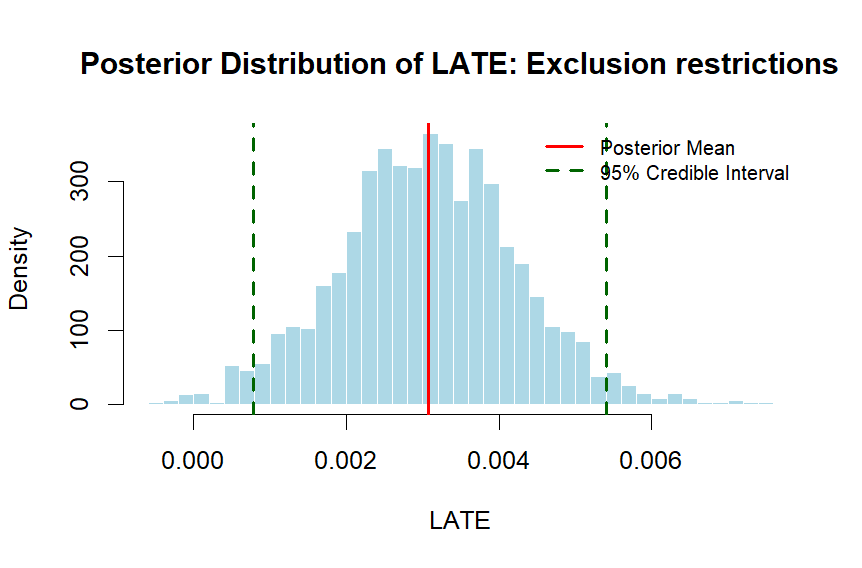
\includegraphics[width=340pt, height=200pt]{Chapters/chapter12/figures/LATE.png}
	\caption[List of figure caption goes here]{Posterior distribution: Local average average atreatment effect vitamin A supplements.}\label{fig12_LATE}
\end{figure}


\textbf{Example: Treatment effect of 401(k) participation on net financial assets}

In the example of the effect of \textit{eligibility} on 401(k) on net financial assets, we calculate the ITT effect. Now, following \cite{chernozhukov2004effects}, we use eligibility as an instrument for \textit{participation} and perform inference on the (local) average treatment effect. We adopt the framework described in Section \ref{sec73} for this example. The following code illustrates the procedure, and Figure \ref{fig12_3} displays the posterior distribution of the (local) average treatment effect of participation. The 95\% credible interval is (USD 5,102, USD 12,010), and the posterior mean is USD 8,520, which is higher than the intention-to-treat effect associated with eligibility (USD 5,903). 

Exercise~6 asks how to recover the ITT from the LATE and the effect of eligibility on participation. See \cite{Conley2012} for practical methods to conduct sensitivity analysis of posterior results when relaxing the exclusion restriction in IV settings. In addition, \cite{conley2008semi} present a Bayesian inferential framework using a semi-parametric approach in which stochastic errors are modeled using a Dirichlet process (see Exercise 7), and \cite{ramirez2024welfare} extend this approach to systems of equations.

\begin{tcolorbox}[enhanced,width=4.67in,center upper,
	fontupper=\large\bfseries,drop shadow southwest,sharp corners]\label{code3n_chap12}
	\textit{R code. Treatment effect: 401(k) participation on net financial assets}
	\begin{VF}
		\begin{lstlisting}[language=R]		
rm(list = ls()); set.seed(10101)
library(coda); library(ggplot2)
mydata <- read.csv("https://raw.githubusercontent.com/BEsmarter-consultancy/BSTApp/refs/heads/master/DataApp/401k.csv", sep = ",", header = TRUE, quote = "")
# Attach variables
attach(mydata)
y <- net_tfa/1000  # Outcome: net financial assets
x <- as.vector(p401) # Endogenous regressor: participation
w <- as.matrix(cbind(1, age, inc, fsize, educ, marr, twoearn, db, pira, hown))  # Exogenous regressors with intercept
z <- as.matrix(e401)  # Instrument: eligibility (NO intercept here)
X <- cbind(x, w); Z <- cbind(z, w)
# Dimensions
k <- ncol(X); kz <- ncol(Z)  
# Priors
b0 <- rep(0, k); B0i <- diag(1e-5, k)
g0 <- rep(0, kz); G0i <- diag(1e-5, kz)
nu <- 3; Psi0 <- nu * 1000 * diag(2); Psi0i <- solve(Psi0)
# MCMC parameters
mcmc <- 5000; burnin <- 1000
tot <- mcmc + burnin; thin <- 1
# Auxiliary elements
XtX <- t(X)%*%X; ZtZ <- t(Z)%*%Z; nun <- nu + length(y)
# Gibbs sampling
PostBeta <- function(Sigma, Gamma){
	w1 <- Sigma[1,1] - Sigma[1,2]^2/Sigma[2,2]
	Bn <- solve(w1^(-1)*XtX + B0i)
	yaux <- y - (Sigma[1,2]/Sigma[2,2])*(x - Z%*%Gamma)
	bn <- Bn%*%(B0i%*%b0 + w1^(-1)*t(X)%*%yaux)
	Beta <- MASS::mvrnorm(1, bn, Bn)
	return(Beta)
}
PostGamma <- function(Sigma, Beta){
	w2 <- Sigma[2,2] - Sigma[1,2]^2/Sigma[1,1]
	Gn <- solve(w2^(-1)*ZtZ + G0i)
	xaux <- x - (Sigma[1,2]/Sigma[1,1])*(y - X%*%Beta)
	gn <- Gn%*%(G0i%*%g0 + w2^(-1)*t(Z)%*%xaux)
	Gamma <- MASS::mvrnorm(1, gn, Gn)
	return(Gamma)
}
PostSigma <- function(Beta, Gamma){
	Uy <- y - X%*%Beta; Ux <- x - Z%*%Gamma
	U <- cbind(Uy, Ux)
	Psin <- solve(Psi0i + t(U)%*%U)
	Sigmai <- rWishart::rWishart(1, df = nun, Sigma = Psin)
	Sigma <- solve(Sigmai[,,1]) 
	return(Sigma)
}
	\end{lstlisting}
	\end{VF}
\end{tcolorbox} 

\begin{tcolorbox}[enhanced,width=4.67in,center upper,
	fontupper=\large\bfseries,drop shadow southwest,sharp corners]\label{code3_chap12}
	\textit{R code. Treatment effect: 401(k) participation on net financial assets}
	\begin{VF}
		\begin{lstlisting}[language=R]		
PostBetas <- matrix(0, tot, k)
PostGammas <- matrix(0, tot, kz)
PostSigmas <- matrix(0, tot, 2*(2+1)/2)
Beta <- rep(0, k); Gamma <- rep(0, kz)
pb <- txtProgressBar(min = 0, max = tot, style = 3)
for(s in 1:tot){
	Sigma <- PostSigma(Beta = Beta, Gamma = Gamma)
	Beta <- PostBeta(Sigma = Sigma, Gamma = Gamma)
	Gamma <- PostGamma(Sigma = Sigma, Beta = Beta)
	PostBetas[s,] <- Beta
	PostGammas[s,] <- Gamma
	PostSigmas[s,] <- matrixcalc::vech(Sigma)
	setTxtProgressBar(pb, s)
}
close(pb)
keep <- seq((burnin+1), tot, thin)
Bs <- PostBetas[keep,]
Gs <- PostGammas[keep,]
Sigmas <- PostSigmas[keep,]
summary(coda::mcmc(Bs))
summary(coda::mcmc(Gs))
summary(coda::mcmc(Sigmas))
# Extract posterior draws for the treatment effect (participation = p401)
beta_draws <- Bs[,1]
# Plot posterior distribution of treatment effect
df_beta <- data.frame(effect = as.vector(beta_draws))
ggplot(df_beta, aes(x = effect)) + geom_density(fill = "steelblue", alpha = 0.6) +
geom_vline(xintercept = mean(beta_draws), color = "red", linetype = "dashed", linewidth = 1) + labs( title = "Posterior Distribution of 401(k) Participation Effect", x = expression(beta["p401"]), y = "Density") + theme_minimal(base_size = 14)
\end{lstlisting}
	\end{VF}
\end{tcolorbox}  
 
\begin{figure}[h!]
	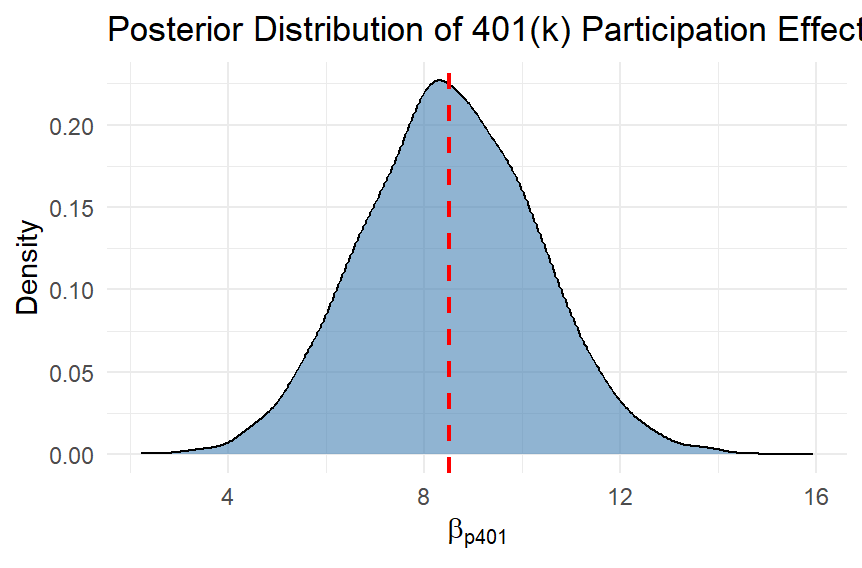
\includegraphics[width=340pt, height=200pt]{Chapters/chapter12/figures/FigP401k.png}
	\caption[List of figure caption goes here]{Posterior distribution: Local average treatment effect 401k participation on net financial assets.}\label{fig12_3}
\end{figure}

\section{Difference-in-differences design (DiD)}\label{sec12_5}

In this section, we present how to perform inference and discuss the identification conditions when working with panel (longitudinal) data or repeated cross-sectional data in the \textit{difference-in-differences} (DiD) framework. In DiD designs, we estimate causal effects by comparing changes over time between groups that receive the treatment and groups that do not (the ``control'' group). This approach is among the most widely used designs for identifying causal effects \cite{baker2025did_guide}. Its origins can be traced back to John Snow, the father of modern epidemiology, who in 1855 analyzed the spread of cholera through water in London \cite{chernozhukov2024applied}.

In what follows, we first present the basic two-group, two-period ($2\times2$) DiD setup, and then introduce the staggered DiD design.

\subsection{Classic DiD: two-group and two-period ($2\times2$) setup}\label{sec12_51}

Following \cite{roth2023whats}, we consider a setting with two time periods, \( t = 1, 2 \), and two groups: a treated group (\( D_i = 1 \)) that receives the treatment between periods \( t = 1 \) and \( t = 2 \), and a control group that never receives the treatment (\( D_i = 0 \)). We observe outcomes \( Y_{it} \) and treatment status \( D_i \) for units \( i = 1, 2, \dots, N \), assuming a balanced panel data structure.

Let \( Y_{it}(1) \) denote the potential outcome for unit \( i \) in period \( t \) if it is untreated in the first period and treated in the second, while \( Y_{it}(0) \) denotes the potential outcome if it is never treated. In the DiD framework, the primary estimand of interest is the average treatment effect on the treated (ATT),
\[
\tau_{2} = \mathbb{E}[Y_{i2}(1) - Y_{i2}(0) \mid D_i = 1].
\]

Note that we do not observe \( Y_{i2}(0) \mid D_i = 1 \); that is, the outcome in the second period for treated units if they had not received the treatment. Thus, the identification conditions in DiD are designed to express this counterfactual outcome as a function of the data.

There are two key identification assumptions:

\textit{1. Parallel trends:}
\begin{equation}
	\mathbb{E}[Y_{i2}(0) - Y_{i1}(0) \mid D_i = 1] = \mathbb{E}[Y_{i2}(0) - Y_{i1}(0) \mid D_i = 0],
\end{equation}
which states that, in the absence of treatment, the average change in outcomes for the treated and control groups would have evolved similarly over time.

\textit{2. No anticipation effects:}
\begin{equation}
	\mathbb{E}[Y_{i1}(0)\mid D_i=1] = \mathbb{E}[Y_{i1}(1)\mid D_i=1],
\end{equation}
meaning that the treatment has no causal effect prior to its implementation.

Thus, we can use the parallel trends assumption to express \( \mathbb{E}[Y_{i2}(0) \mid D_i = 1] \) as
\begin{align*}
	\mathbb{E}[Y_{i2}(0)\mid D_i = 1] 
	&= \mathbb{E}[Y_{i1}(0) \mid D_i = 1] + \mathbb{E}[Y_{i2}(0) - Y_{i1}(0) \mid D_i = 0] \\
	&= \mathbb{E}[Y_{i1}(1) \mid D_i = 1] + \mathbb{E}[Y_{i2}(0) - Y_{i1}(0) \mid D_i = 0] \\
	&= \mathbb{E}[Y_{i1} \mid D_i = 1] + \mathbb{E}[Y_{i2} - Y_{i1} \mid D_i = 0],
\end{align*}
where the second equality follows from the no anticipation effects assumption.

Therefore,
\begin{equation}\label{eq:DiD}
\tau_2 = \mathbb{E}[Y_{i2} - Y_{i1} \mid D_i = 1] - \mathbb{E}[Y_{i2} - Y_{i1} \mid D_i = 0],
\end{equation}
that is, the ATT is the difference in outcome differences between treated and control units. 

Figure \ref{Fig:DiD} shows a graphical representation of the identification assumptions in DiD \cite{chernozhukov2024applied}. \cite{normington2022bayesian} show a DAG representation of DiD.

\begin{figure}[ht]
	\centering
	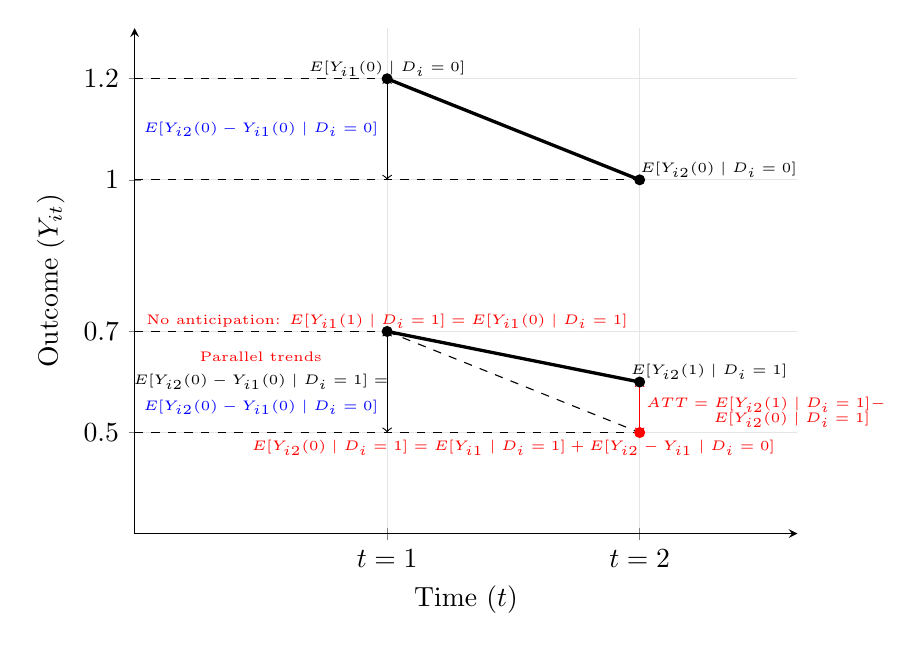
\begin{tikzpicture}
		\begin{axis}[
			width=10cm,height=8cm,
			xmin=-0.6, xmax=1.5, ymin=0.3, ymax=1.3,
			axis lines=left,
			grid=both, grid style={gray!20},
			xlabel={Time ($t$)},
			ylabel={Outcome ($Y_{it}$)},
			xtick={0.2, 1}, xticklabels={$t=1$, $t=2$},
			ytick={0.5, 0.7, 1, 1.2},
			clip=false
			]
			% Sharp RD step:
			\addplot[dashed] coordinates {(-0.6,0.5) (1,0.5)};
			\addplot[dashed] coordinates {(-0.6,0.7) (0.2,0.7)};
			
			\addplot[black, very thick] coordinates {(0.2,0.7) (1,0.6)};
			\addplot[dashed] coordinates {(0.2,0.7) (1,0.5)};
			\draw[<->] (axis cs:0.2,0.7) -- (axis cs:0.2,0.5);
			\node[red] at (axis cs:-0.2,0.65) {\tiny Parallel trends};
			\node[black] at (axis cs:-0.2,0.6) {\tiny $\mathbb{E}[Y_{i2}(0) - Y_{i1}(0) \mid D_i = 1] = $};
			\node[blue] at (axis cs:-0.2,0.55) {\tiny $ \mathbb{E}[Y_{i2}(0) - Y_{i1}(0) \mid D_i = 0]$};
			
			\addplot[dashed] coordinates {(-0.6,1) (1,1)};
			\addplot[dashed] coordinates {(-0.6,1.2) (0.2,1.2)};
			
			\addplot[black, very thick] coordinates {(0.2,1.2) (1,1)};
			\draw[<->] (axis cs:0.2,1.2) -- (axis cs:0.2,1);
			\node[blue] at (axis cs:-0.2,1.1) {\tiny $\mathbb{E}[Y_{i2}(0) - Y_{i1}(0) \mid D_i = 0]$};
			\node[black] at (axis cs:0.2,1.22) {\tiny $\mathbb{E}[Y_{i1}(0) \mid D_i = 0]$};
			\node[black] at (axis cs:1.25,1.02) {\tiny $\mathbb{E}[Y_{i2}(0) \mid D_i = 0]$};
			\node[red] at (axis cs:0.2,0.72) {\tiny No anticipation: $\mathbb{E}[Y_{i1}(1) \mid D_i = 1]=\mathbb{E}[Y_{i1}(0) \mid D_i = 1]$};
			\node[black] at (axis cs:1.22,0.62) {\tiny $\mathbb{E}[Y_{i2}(1) \mid D_i = 1]$};
			\draw[<->, red] (axis cs:1,0.6) -- (axis cs:1,0.5);
			\node[red] at (axis cs:1.4,0.555) {\tiny $ATT=\mathbb{E}[Y_{i2}(1) \mid D_i = 1]-$};
			\node[red] at (axis cs:1.482,0.525) {\tiny $\mathbb{E}[Y_{i2}(0) \mid D_i = 1]$};
			\node[red] at (axis cs:0.6,0.47) {\tiny $\mathbb{E}[Y_{i2}(0) \mid D_i = 1]=\mathbb{E}[Y_{i1} \mid D_i = 1] + \mathbb{E}[Y_{i2} - Y_{i1} \mid D_i = 0]$};
			
			\fill[black] (axis cs:0.2,1.2) circle (2pt);
			\fill[black] (axis cs:1,1) circle (2pt);
			\fill[black] (axis cs:0.2,0.7) circle (2pt);
			\fill[black] (axis cs:1,0.6) circle (2pt);
			\fill[red] (axis cs:1,0.5) circle (2pt);
			%\draw[black, fill=black] (0.7,1) circle (2pt);
			%\draw[black, fill=black] (0.2,0.7) circle (2pt);
			%\draw[black, fill=black] (0.7,0.6) circle (2pt);
			% Cutoff (vertical dashed line)
			%\addplot[black, densely dashed, very thick] coordinates {(0,0) (0,1.02)};
			
			% Labels
			%\node[black] at (axis cs:-0.52,0.92) {\large Assigned to Control};
			%\node[black]  at (axis cs: 0.52,0.92) {\large Assigned to Treatment};
			
			% Arrow and text to mark "Cutoff"
			%\draw[->] (axis cs:0.28,0.2) -- (axis cs:0.02,0.2);
			%\node[anchor=west] at (axis cs:0.3,0.2) {Cutoff};
			
			% Bracket showing jump size (optional)
			%\draw[<->, thick] (axis cs:0.04,0.0) -- (axis cs:0.04,1);
			%\node[anchor=west] at (axis cs:0.06,0.50) {$\Delta P$};
		\end{axis}
	\end{tikzpicture}
	\caption{Difference-in-Differences: Identification strategy}
	\label{Fig:DiD}
\end{figure}

Note that we can express the observed outcome in terms of potential outcomes as
\[
Y_{it} = Y_{it}(0) + \big[\,Y_{it}(1) - Y_{it}(0)\,\big] D_i.
\]
Therefore,
\[
Y_{i1} = Y_{i1}(0) + \big[\,Y_{i1}(1) - Y_{i1}(0)\,\big] D_i,
\]
and
\[
Y_{i2} = Y_{i2}(0) + \big[\,Y_{i2}(1) - Y_{i2}(0)\,\big] D_i.
\]
Subtracting the first equation from the second yields
\[
Y_{i2} - Y_{i1} = \underbrace{Y_{i2}(0) - Y_{i1}(0)}_{\text{common trend}} 
+ \underbrace{\big[(Y_{i2}(1) - Y_{i1}(1)) - (Y_{i2}(0) - Y_{i1}(0))\,\big]}_{\text{treatment effect in changes}} D_i.
\]

Under the \emph{parallel trends} assumption, the expected value of the common trend is the same for treated and control units. This assumption is compatible with the linear CEF function
\[
Y_{it} = \alpha_i + \phi_t + \tau_2 D_i + \mu_{it},
\]
which implies
\[
Y_{i2} - Y_{i1} = (\phi_2 - \phi_1) + \tau_2 D_i + (\mu_{i2} - \mu_{i1}).
\]
Comparing this expression with the one derived from the potential outcomes framework, it follows that regressing the time difference $Y_{i2} - Y_{i1}$ on a constant and the treatment indicator $D_i$ identifies $\tau_2$, the ATT.

Another common formulation in the linear regression setting that recovers the ATT is the two-way fixed effects (TWFE) model
\[
Y_{it} = \alpha + \alpha_i + \phi_t + \tau_2 \,\big[ D_i \cdot \mathbbm{1}(t = 2) \big] + \epsilon_{it},
\]
where $\mathbbm{1}(t = 2)$ is an indicator for the post-treatment period \cite{roth2023whats}. The advantage of the regression setting is that it allows for the straightforward calculation of the standard error of the ATT, enabling the construction of confidence or credible intervals under the Frequentist and Bayesian approaches, respectively.

The DiD framework can be extended to condition on covariates. In this case, we assume that the underlying identification assumptions are more plausible among units that are similar in terms of observed characteristics. Thus, the identification assumptions are stated conditional on the exogenous variables.

Therefore, we can use covariates to assess the balance between control and treated groups in terms of levels ($X$) or differences ($\Delta X$) before and after treatment:
\[
\frac{\bar{X}_1-\bar{X}_2}{\sqrt{\hat{\sigma}_1^2+\hat{\sigma}_2^2}},
\] 
where $\hat{\sigma}_l^2$ is the sample variance of $X_l$, $l=\left\{1,2\right\}$. 
As a rule of thumb, absolute standardized differences greater than 0.25 indicate potentially problematic imbalance \cite{baker2025did_guide}. Imbalance in covariates can lead to violations of the parallel trends assumption if these covariates would generate different outcomes under the counterfactual scenarios.

In this setting, the \textit{conditional parallel trends} assumption becomes
\begin{equation}
	\mathbb{E}[Y_{i2}(0) - Y_{i1}(0) \mid D_i = 1, \mathbf{X}_i] 
	= \mathbb{E}[Y_{i2}(0) - Y_{i1}(0) \mid D_i = 0, \mathbf{X}_i], \ \text{almost surely}
\end{equation}
and the \textit{no anticipation} assumption becomes
\begin{equation}
	\mathbb{E}[Y_{i1}(0) \mid D_i = 1, \mathbf{X}_i] 
	= \mathbb{E}[Y_{i1}(1) \mid D_i = 1, \mathbf{X}_i].
\end{equation} 
In addition, the \textit{overlap} assumption is required: there exists a treatment group whose characteristics overlap with those of the control group,
\[
P(D_i = 1 \mid \mathbf{X}_i) < 1 - \epsilon, \ \epsilon >0, \ \text{almost surely, and,} \ P(D_i=1)>0.
\]

Following similar arguments as before, we obtain the \textit{conditional average treatment effect on the treated} (CATT) \cite{baker2025did_guide}:
\[
\tau_2(\mathbf{X}_i)= \mathbb{E}[Y_{i2} - Y_{i1} \mid D_i = 1, \mathbf{X}_i] - \mathbb{E}[Y_{i2} - Y_{i1} \mid D_i = 0, \mathbf{X}_i].
\]
The overall ATT can then be recovered by averaging over the distribution of $\mathbf{X}_i$ in the treated population:
\begin{align*}
	\tau_2 & = \mathbb{E}_{\mathbf{X}}\left\{\mathbb{E}[Y_{i2} - Y_{i1} \mid D_i = 1, \mathbf{X}_i] - \mathbb{E}[Y_{i2} - Y_{i1} \mid D_i = 0, \mathbf{X}_i] \mid D_i = 1\right\}\\
	&=\mathbb{E}[Y_{i2} - Y_{i1} \mid D_i = 1]-\mathbb{E}_{\mathbf{X}}\left\{\mathbb{E}[Y_{i2} - Y_{i1} \mid D_i = 0, \mathbf{X}_i]\mid D_i=1\right\},
\end{align*}
where the second line uses the law of iterated expectations:
\[
\mathbb{E}_{\mathbf{X}\mid D=1}\!\left( \mathbb{E}[Y_{i2}-Y_{i1} \mid D=1, \mathbf{X}_i] \right) 
= \mathbb{E}[Y_{i2}-Y_{i1} \mid D=1].
\]

Assuming a linear CEF and a homogeneous ATT, that is, treatment effects do not vary across $\mathbf{X}_{it}$, we can use the first–difference specification,
\[
\Delta Y_{i2} = \alpha + \beta D_i + \sum_{k=1}^K \beta_k \Delta X_{ik2} + \Delta\mu_{i2},
\]
where $\Delta Y_{i2} = Y_{i2} - Y_{i1}$ and $\Delta X_{ik2} = X_{ik2} - X_{ik1}$. This specification identifies the ATT under the homogeneity assumption, in which case $\tau_2 = \beta$; otherwise, it identifies a weighted average of the conditional ATTs across covariates, with the possibility of negative weights that do not sum to one (\textit{non-convex weights}) \cite{baker2025did_guide}.

An alternative specification is the TWFE
\begin{align*}
	Y_{it} & = \alpha + \alpha_i + \phi_t + \beta (\mathbbm{1}(t=2)\cdot D_i) +   \sum_{k=1}^K \beta_k (\mathbbm{1}(t=2)\cdot X_{ik1})\\
	& +  \sum_{k=1}^K \delta_k (\mathbbm{1}(t=2)\cdot D_i \cdot X_{ik1}) + \epsilon_{it}.
\end{align*}

This specification can identify heterogeneous ATT under the assumption of a linear CEF.

%For instance, \cite{normington2019bayesian,normington2022bayesian} use the first–difference specification to implement DiD in a Bayesian hierarchical framework, given the data structure they faced.

However, alternative \textit{semiparametric} and \textit{nonparametric} approaches, such as \textit{outcome regression adjustment}, \textit{inverse probability weighting}, and \textit{doubly robust} estimators (which combine the first two), are often preferable because they yield consistent estimates under conditional parallel trends without requiring a linear conditional expectation function (CEF) \cite{abadie2005semiparametric,roth2023whats}. These approaches typically involve two stages: first, estimating either the conditional mean of the outcome or the propensity score (probability of treatment; \cite{rosenbaum1983central}), and second, using these estimates in a plug-in step to perform inference on the ATT. For Bayesian doubly robust frameworks for average treatment effects, see \cite{SaarelaBelzileStephens2016,YiuGoudieTom2020,LuoGrahamMcCoy2023,breunig2025double} and Section \ref{sec12_11}.

A point to be aware of when performing DiD identification strategies is that the parallel trends assumption is generally not robust to functional form transformations of the outcome. That is, it may hold when the outcome is measured in levels but fail when it is expressed in logarithms. This is because two groups can have the same absolute increase (parallel trends in levels) but different percentage increases (non-parallel in logs).

Note that the parallel trends and no anticipation assumptions in DiD are not fundamentally testable, since they are identifying restrictions about counterfactual outcomes that are never observed. However, we can examine pre-treatment dynamics to assess their plausibility. For instance, we can check for pre-existing differences in trends (``pre-trends'') as a diagnostic for the parallel trends assumption.  

Given a pre-treatment period $t=0$, the no anticipation assumption implies that 
\[
\mathbb{E}[Y_{it}(0)] = \mathbb{E}[Y_{it}] \quad \text{for all } i \text{ and } t \leq 0.
\]
Thus, one can test whether
\begin{equation}
	\mathbb{E}[Y_{i1}(0) - Y_{i0}(0) \mid D_i = 1] 
	= \mathbb{E}[Y_{i1}(0) - Y_{i0}(0) \mid D_i = 0],
\end{equation}
which corresponds to checking for differences in pre-treatment trends between treated and control groups.

The results of such tests should be interpreted with caution. Even if pre-trends are perfectly parallel, this does not guarantee that the parallel trends assumption will hold in the post-treatment period. Moreover, there may be power issues: a true pre-existing difference in trends may go undetected if pre-treatment estimates are imprecise due to high variability.

In addition, one can conduct placebo tests by pretending that the policy started earlier and checking whether a spurious effect is detected prior to the true start. This provides indirect evidence on the plausibility of the no anticipation assumption.

Therefore, it is advisable to complement pre-trend diagnostics with sensitivity analyses, incorporating context-specific knowledge about plausible confounding factors.

\subsection{Staggered (SDiD): G-group and T-period ($G\times T$) setup}\label{chap12_52}

Many empirical settings are more complex than the two-period, two-group ($2\times 2$) design. Nevertheless, even in such settings we can view the design as an aggregation of $2\times 2$ comparisons between units that receive treatment and units that are not yet treated at the relevant time \cite{baker2025did_guide}.

In a setting with multiple periods and different groups, assuming that treatment is an absorbing state —that is, once treated, units remain treated— staggered DiD (SDiD) analyses seek to estimate a weighted average of heterogeneous ATTs, where the weights may be based on economic/policy relevance. 

Given $t = 1, 2, \dots, T$, a unit can be treated at $t = g > 1$,  
\[
Y_{it}(g) := Y_{it}\big(\underbrace{0, \dots, 0}_{g-1}, \underbrace{1, \dots, 1}_{T-g+1}\big)
\]
denotes the potential outcome path for a unit treated at $g$, and
\[
Y_{it}(\infty) := Y_{it}\big(\underbrace{0, \dots, 0}_{T}\big)
\]
denotes the potential outcome path for a never-treated unit.  
Under the absorbing treatment assumption, $D_{it} = 1$ for all $t \geq g$. Let
\[
G_i = \min\left\{ t : D_{it} = 1 \right\}
\]
denote the first period in which unit $i$ is treated.

The average treatment effect for units first treated in period $g$ at time $t$ is
\[
ATT(g,t) = \mathbb{E}\left[ Y_{it}(g) - Y_{it}(\infty) \,\middle|\, G_i = g \right].
\]

Therefore, each cohort $g$ has its own $T-1$ ATT estimands. Each $ATT(g,t)$ represents the average treatment effect of initiating treatment in period $g$, relative to never receiving treatment.

The identifying assumptions for $ATT(g,t)$ are:

\textit{1. Staggered parallel trends based on not-yet-treated units}:
\begin{equation}\label{eq:SDiDNY}
	\mathbb{E}[Y_{it}(\infty) - Y_{it-1}(\infty) \mid G_i = g] 
	= \mathbb{E}[Y_{it}(\infty) - Y_{it-1}(\infty) \mid G_i = g'], \quad \forall\, t \geq g, g'>t.
\end{equation}
The \textit{not-yet-treated} staggered parallel assumption establishes that the average change in potential outcomes for all treated groups would have evolved in parallel after treatment began, under the counterfactual scenario in which they had not received treatment.

Note that the \textit{not-yet-treated} parallel trends assumption can be modified to use \textit{never-treated} units as the comparison group (replace $g'$ by $\infty$ in Equation~\ref{eq:SDiDNY}), or to impose parallel trends across \textit{all} groups and periods (no restrictions on $g$ and $g'$). The \textit{all-groups, all-periods} version is more demanding but can yield more precise estimates because it exploits a larger set of observations. In contrast, the \textit{never-treated} version requires fewer assumptions about parallel trends but is typically less precise. The \textit{not-yet-treated} version represents a middle ground between these two. Ultimately, the choice of which parallel trends assumption to adopt is context-specific \cite{baker2025did_guide}.

\textit{2. Staggered no anticipation}:
\begin{equation*}
	\mathbb{E}[Y_{it}(g)] = \mathbb{E}[Y_{it}(\infty)], \quad \forall\, i,\ t < g.
\end{equation*}

That is, treated units do not change their potential outcomes in anticipation of future treatment before treatment begins.

Thus, to identify long-term effects, the parallel trends assumption must hold for all periods after the earliest treatment period in the not-yet-treated case. If the goal is to estimate effects in a specific short-term period, parallel trends must hold in that period.

Note that under these assumptions, we can express $ATT(g,t)$ in terms of observable outcomes as \cite{roth2023whats}
\begin{align*}
	ATT(g,t) 
	= \mathbb{E}\big[ Y_{it} - Y_{i, g-1} \mid G_i = g \big]
	- \mathbb{E}\big[ Y_{it} - Y_{i, g-1} \mid G_i = g', \ g' > t \big].
\end{align*}
This formulation makes explicit the choice of the comparison group, either not-yet-treated or never-treated units in this setting. Moreover, cohorts are indexed by the first treatment date $g$, and effects are evaluated at calendar time $t$. Hence the object of interest is cohort–time specific, $ATT(g,t)$, and staggered designs generally imply a multiplicity of ATT parameters, where each estimand can be seen as a multi-period version of a DiD causal effect (Equation~\ref{eq:DiD}).

To study the dynamics of treatment effects, we can use \textit{event study} plots. These involve estimating and reporting effects for a range of periods before and after treatment, allowing us to analyze the temporal pattern of the ATTs \cite{baker2025did_guide}. 

%In this context, we can perform inference on
%\[
%ATT_l^w = \sum_g w_g \, ATT(g, g+l),
%\]
%where $w_g$ denotes the weight for cohort $g$. For instance, if the outcome variable is defined at the school level (e.g., the proportion of dropouts), then $ATT(g,t)$ is a school-level effect, and $w_g$ could be the proportion of students in that school relative to the total student population.\footnote{In general, given a hierarchical structure, all the expected values in this section can be defined as $w$-weighted population expectations; see \cite{baker2025did_guide}.}
%
%Here, $Y_{it}(g)$ denotes the potential outcome for unit $i$ at time $t$ if treated at $g$, and $Y_{it}(\infty)$ denotes the potential outcome if never-treated. For units not yet treated by period $t = g$, $Y_{it} = Y_{it}(0)$; for units treated in period $t = g$, $Y_{it} = Y_{it}(1)$ for all $t \ge g$ under the absorbing treatment assumption.  
%
%These weights can be constructed in several ways depending on the aggregation scheme and the estimand of interest \cite{goodman2021difference}. For example, $w$ can be based on:
%\begin{enumerate}
%	\item \textbf{Unit counts}: the number of observations in the treated and control groups within each comparison.
%	\item \textbf{Population shares}: the proportion of the population (e.g., students, residents) in the treated and control groups.
%	\item \textbf{Variance weights}: inverse-variance weights reflecting the precision of each $2\times2$ comparison.
%\end{enumerate}
%Note that, regardless of the weighting scheme, clustering must be taken into account when quantifying uncertainty, especially when treatment is assigned at the higher-level unit.

An advantage of having multiple pre-treatment periods in the design is that it allows calculating \textit{falsification/placebo tests}. Under the \textit{no anticipation} assumption, any potential effect before $G_i$ must be zero. That is, given $b < \min\{g,g'\}$, for all $t \text{ with } b < t < \min\{g,g'\}$: 
\[
\mathbb{E}\!\left[\,Y_{it}-Y_{ib}\mid G_i=g\right]
=
\mathbb{E}\!\left[\,Y_{it}-Y_{ib}\mid G_i=g'\right].
\]

Thus, we can test whether the differences in the expected changes of the outcome variable before treatment between different groups are statistically indistinguishable from zero. If this is the case, common practice would suggest that there is evidence in favor of parallel trends. However, we should remember that the parallel trends assumption is essentially untestable because it imposes restrictions on post-treatment periods, not on pre-treatment periods. Consequently, the same recommendations as those at the end of the previous section apply: perform sensitivity analyses regarding potential violations of the parallel trends assumption.

Assuming that parallel trends hold conditional on covariates, we obtain identification under the following assumptions:

\textit{1. Staggered parallel trends with not-yet-treated comparison (conditional on $\mathbf X_i$):}
\[
\mathbb{E}\!\left[Y_{it}(\infty)-Y_{i,t-1}(\infty)\mid G_i=g,\ \mathbf X_i\right]
=
\mathbb{E}\!\left[Y_{it}(\infty)-Y_{i,t-1}(\infty)\mid G_i>t,\ \mathbf X_i\right],
\quad \forall\, g,\ t<g.
\]

\textit{2. Staggered overlap (positivity) for not-yet-treated comparisons:}
\[
\epsilon \le P(G_i=g \mid \mathbf X_i)
\quad \text{and} \quad
\epsilon \le P(G_i>t \mid \mathbf X_i),
\quad \forall\, g,\ t<g,\ \text{for some } \epsilon>0.
\]

Condition 1 means that conditional on covariates, pre-treatment changes in untreated potential outcomes for cohort $g$ match those of units not yet treated at time $t$, and condition 2 means that there is positive probability of belonging to cohort $g$ and of being not yet treated at $t$.

Given these assumptions and no anticipation, the $ATT(g,t)$ can be expressed as
\begin{align*}
	ATT(g,t) &=\mathbb{E}[Y_{it} - Y_{ig-1} \mid G_i = g]-\mathbb{E}_{\mathbf{X}}\left\{\mathbb{E}[Y_{it} - Y_{ig-1} \mid\mathbf{X}_i,  G_i = g'>t]\mid G_i=g\right\}.
\end{align*}

Again, inference on $ATT(g,t)$ can be conducted using regression adjustment, inverse-probability weighting, or doubly robust estimators. Although TWFE specifications are often used to estimate $ATT(g,t)$, \cite{baker2025did_guide} recommend avoiding them in staggered DiD settings because they generally do not identify $ATT(g,t)$. Instead, they recover a complicated, non-convex weighted average of cohort–time effects, with potentially negative weights.\\

\textbf{Example: Difference-in-Differences simulation}

Let's simulate a DiD setting where the treatment effect is $1$ and the common trend is $-1.8$. We assume the default priors in the \textit{MCMCpack} package. We perform inference on the ATT using

\[
Y_{i2} - Y_{i1}
= \underbrace{\phi_2 - \phi_1}_{\text{Common change}}
+ \tau_2 D_i + \epsilon_i.
\]

The following code implements this example. From the posterior results, we can verify that the 95\% credible interval contains the true ATT. We ask in Exercise~8 to repeat exactly the same simulation, and estimate the ATT using the specification with the interaction between treatment and the post-treatment period.

\begin{tcolorbox}[enhanced,width=4.67in,center upper,
	fontupper=\large\bfseries,drop shadow southwest,sharp corners]
	\textit{R code. Difference-in-Differences: Simulation exercise}
	\begin{VF}
		\begin{lstlisting}[language=R]		
			rm(list = ls()); set.seed(10101)
			library(ggplot2); library(dplyr); library(fastDummies)
			# Parameters
			N_per_group <- 200          # units per group
			T_periods    <- 2           # keep 2x2 for clarity
			tau_true     <- 1           # ATT
			sigma_eps    <- 0.5         # noise SD
			# Panel index
			id  <- rep(1:(2*N_per_group), each = T_periods)
			t   <- rep(1:T_periods, times = 2*N_per_group)
			# Group: treated (D=1) vs control (D=0)
			D   <- rep(c(rep(0, N_per_group), rep(1, N_per_group)), each = T_periods)
			# Post indicator (t=2 is post)
			post <- as.integer(t == 2)
			# Unit fixed effects (random heterogeneity)
			alpha_i <- rnorm(2*N_per_group, 0, 0.8)
			alpha   <- alpha_i[id]
			# Time effects (common shocks)
			phi_t <- c(0, -1.8)  # common decline from t=1 to t=2
			phi   <- phi_t[t]
			treat_effect <- tau_true * (D * post)
			# Outcome:
			eps <- rnorm(length(id), 0, sigma_eps)
			Y   <- alpha + phi + treat_effect + eps
			did <- data.frame(id, t, D, post, Y)
			# Bayesian inference: Model in differences
			dY <- did$Y[did$t==2] - did$Y[did$t==1]
			D  <- did$D[did$t==1]
			post_fit <- MCMCpack::MCMCregress(dY ~ 1 + D, burnin = 100, mcmc = 1000)
			tau_draws <- post_fit[, "D"]
			quantile(tau_draws, c(.025,.5,.975))
			quantile(post_fit[,1], c(.025,.5,.975))
		\end{lstlisting}
	\end{VF}
\end{tcolorbox}  

\section{Regression discontinuity design (RD)}\label{chap12_7}

In this section, we study the \textit{regression discontinuity} (RD) design. In particular, we analyze the causal effect of a binary treatment $D_i$ on an outcome $Y_i$ within the potential outcomes (Rubin causal model) framework, namely $Y_i(1)-Y_i(0)$. As usual, we face the fundamental problem of causal inference. Identification in RD relies on a \textit{running variable} $Z_i$, also known as the \textit{forcing}, \textit{index}, or \textit{score variable}, which determines treatment assignment, either completely or partially, depending on whether a unit lies on either side of a known cutoff $c$. The running variable may be associated with the potential outcomes, but this association is assumed to be smooth at $c$. Under this smoothness assumption (and in the absence of precise manipulation at $c$), any discontinuity in the conditional mean of $Y_i$ as a function of $Z_i$ at $c$ identifies the causal effect of the treatment at the cutoff \cite{imbens2008regression}.

There are two common versions of RD: \emph{sharp} and \emph{fuzzy}. In the former, the change (jump) in the conditional probability of treatment at the cutoff equals one; in the latter, it is strictly between zero and one:
\[
\Delta \;=\; \lim_{z \downarrow c}\Pr(D_i=1\mid Z_i=z)-\lim_{z \uparrow c}\Pr(D_i=1\mid Z_i=z)
=
\begin{cases}
	1, & \text{sharp RD},\\[2pt]
	\in(0,1), & \text{fuzzy RD}.
\end{cases}
\]
Here $\lim_{z \downarrow c}$ and $\lim_{z \uparrow c}$ denote the right (approach from above) and left (approach from below) limits, respectively.

\subsection{Sharp regression discontinuity design (SRD)}

In the sharp case, treatment assignment is a deterministic function of the running variable:
\[
D_i = \mathbbm{1}\{Z_i \ge c\},
\]
so the conditional probability of treatment jumps from $0$ to $1$ at $Z_i=c$. All units with $Z_i \ge c$ are treated, whereas those with $Z_i < c$ serve as the control group. Therefore, assignment is identical to treatment in the sharp RD (perfect compliance). Figure \ref{Fig:SRDD} displays the conditional probability of treatment. 

\begin{figure}[ht]
	\centering
	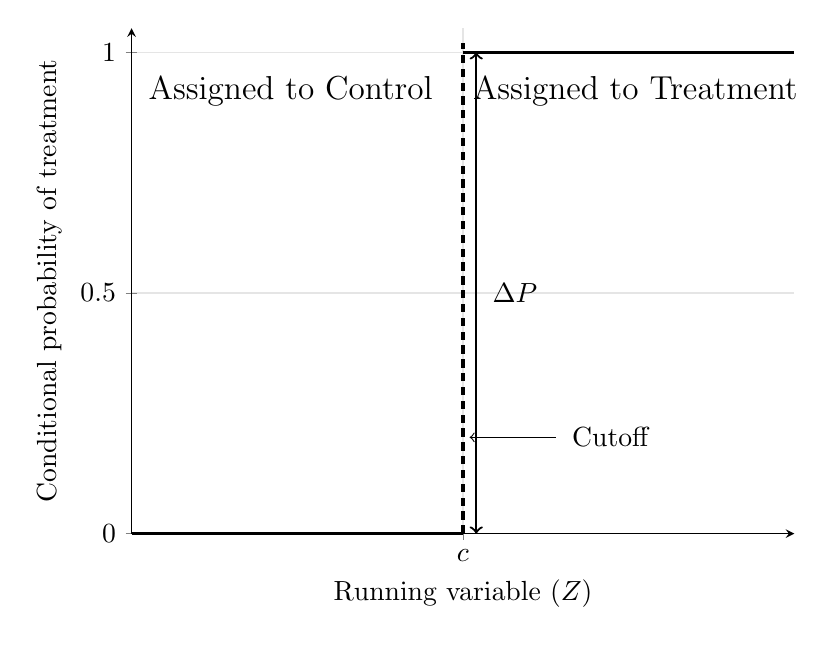
\begin{tikzpicture}
		\begin{axis}[
			width=10cm,height=8cm,
			xmin=-1, xmax=1, ymin=0, ymax=1.05,
			axis lines=left,
			grid=both, grid style={gray!20},
			xlabel={Running variable ($Z$)},
			ylabel={Conditional probability of treatment},
			xtick={0}, xticklabels={$c$},
			ytick={0,0.5,1},
			clip=false
			]
			% Sharp RD step:
			\addplot[very thick] coordinates {(-1,0) (0,0)};
			\addplot[very thick]  coordinates {(0,1) (1,1)};
			
			% Cutoff (vertical dashed line)
			\addplot[black, densely dashed, very thick] coordinates {(0,0) (0,1.02)};
			
			% Labels
			\node[black] at (axis cs:-0.52,0.92) {\large Assigned to Control};
			\node[black]  at (axis cs: 0.52,0.92) {\large Assigned to Treatment};
			
			% Arrow and text to mark "Cutoff"
			\draw[->] (axis cs:0.28,0.2) -- (axis cs:0.02,0.2);
			\node[anchor=west] at (axis cs:0.3,0.2) {Cutoff};
			
			% Bracket showing jump size (optional)
			\draw[<->, thick] (axis cs:0.04,0.0) -- (axis cs:0.04,1);
			\node[anchor=west] at (axis cs:0.06,0.50) {$\Delta P$};
		\end{axis}
	\end{tikzpicture}
\caption{Sharp regression discontinuity design: Conditional probability of treatment}
\label{Fig:SRDD}
\end{figure}

The observed outcome is given by
\begin{align*}
	Y_i=(1-D_i)\cdot Y_i(0) + D_i\cdot Y_i(1)=\begin{Bmatrix}
		Y_i(0), & Z_i < c\\
		Y_i(1), & Z_i \geq c.
	\end{Bmatrix}
\end{align*}

Thus, the causal effect that we target in SRD is
\[
\tau_{SRD}=\mathbb{E}[Y_i(1)-Y_i(0)\mid Z_i=c].
\]

Note that the treatment effect is evaluated at the cutoff, which is a single point in the support of the running variable. Hence $\tau_{\text{SRD}}$ is inherently local and need not be representative of units whose running variable lies far from $c$.
The identification of $\tau_{\text{SRD}}$ requires \emph{continuity of the potential outcome regression functions}, that is,
\[
\mathbb{E}[Y_i(0)\mid Z_i=z]\ \text{and}\ \mathbb{E}[Y_i(1)\mid Z_i=z]
\]
are continuous at $z$. Strictly speaking, it suffices that the left- and right-hand limits of $\mathbb{E}[Y_i(d)\mid Z_i=z]$ coincide at $z=c$ for $d\in\{0,1\}$.

This implies
\begin{align*}
	\mathbb{E}[Y_i(0)\mid Z_i=c]
	&= \lim_{z \uparrow c}\mathbb{E}[Y_i(0)\mid Z_i=z] \\
	&= \lim_{z \uparrow c}\mathbb{E}[Y_i(0)\mid Z_i=z, D_i=0] \\
	&= \lim_{z \uparrow c}\mathbb{E}[Y_i\mid Z_i=z],
\end{align*}
since for $z<c$ we have $D_i=0$. Similarly,
\begin{align*}
	\mathbb{E}[Y_i(1)\mid Z_i=c]
	&= \lim_{z \downarrow c}\mathbb{E}[Y_i(1)\mid Z_i=z] \\
	&= \lim_{z \downarrow c}\mathbb{E}[Y_i\mid Z_i=z],
\end{align*}
because for $z>c$ we have $D_i=1$. Therefore,
\[
\tau_{\text{SRD}}
= \lim_{z \downarrow c}\mathbb{E}[Y_i\mid Z_i=z]
- \lim_{z \uparrow c}\mathbb{E}[Y_i\mid Z_i=z],
\]
i.e., the target estimand is the jump in the conditional mean at the discontinuity point $c$. See Figure \ref{fig:SRD-muplus-muminus}.

\begin{figure}[ht]
	\centering
	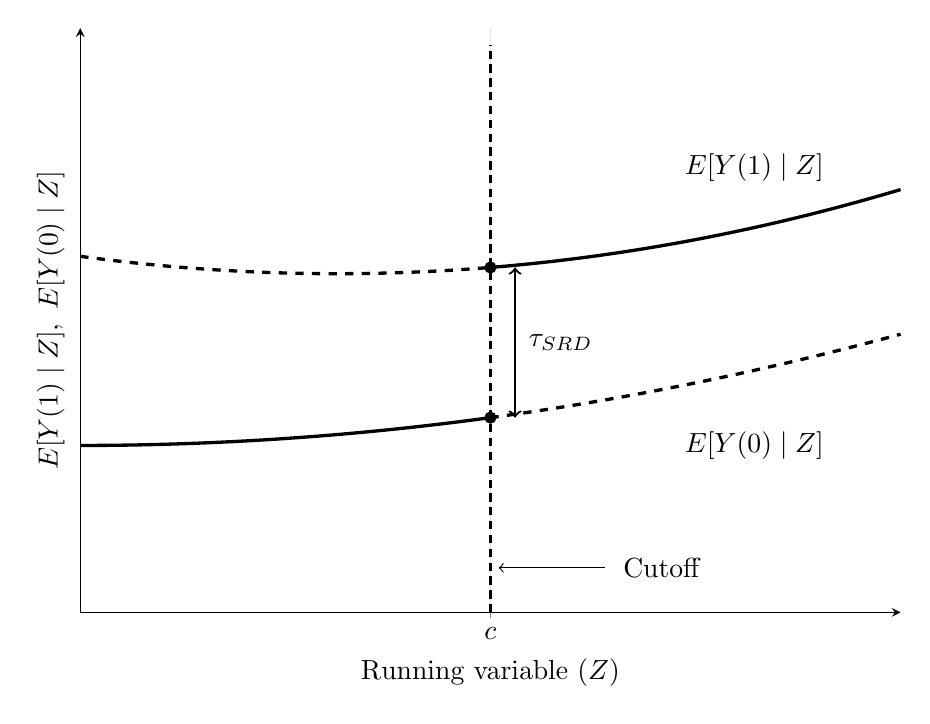
\begin{tikzpicture}
		\begin{axis}[
			width=12cm,height=9cm,
			xmin=-1, xmax=1, ymin=0, ymax=1.05,
			axis lines=left,
			grid=both, grid style={gray!20},
			xlabel={Running variable ($Z$)},
			ylabel={$\mathbb{E}[Y(1)\mid Z],\ \mathbb{E}[Y(0)\mid Z]$},
			xtick={0}, xticklabels={$c$},
			ytick=\empty,
			clip=false
			]
			
			% --- Choose smooth functions for illustration ---
			% E[Y(0)|X]: observed (solid) for X<c, counterfactual (dashed) for X>=c
			\addplot[black, very thick, domain=-1:0, samples=200] {0.35 + 0.1*x + 0.05*x^2};
			\addplot[black, very thick, dashed, domain=0:1, samples=200] {0.35 + 0.1*x + 0.05*x^2};
			
			% E[Y(1)|X]: counterfactual (dashed) for X<c, observed (solid) for X>=c
			\addplot[black, very thick, dashed, domain=-1:0, samples=200] {0.62 + 0.06*x + 0.08*x^2};
			\addplot[black, very thick, domain=0:1, samples=200] {0.62 + 0.06*x + 0.08*x^2};
			
			% --- Cutoff (vertical dashed line) ---
			\addplot[black, densely dashed, very thick] coordinates {(0,0) (0,1.02)};
			
			% --- Points at the cutoff (mu_- and mu_+) ---
			\filldraw[black] (axis cs:0,0.35) circle (2pt);  % mu_-
			\filldraw[black] (axis cs:0,0.62) circle (2pt);  % mu_+
			
			% Labels mu_- and mu_+
			% \node[anchor=east] at (axis cs:-0.02,0.35) {$\mu_-$};
			% \node[anchor=east] at (axis cs:-0.02,0.62) {$\mu_+$};
			
			% --- Jump size tau_SRD ---
			\draw[<->, thick] (axis cs:0.06,0.35) -- (axis cs:0.06,0.62);
			\node[anchor=west] at (axis cs:0.07,0.485) {$\tau_{\text{SRD}}$};
			
			% --- Arrow + label "Cutoff" ---
			\draw[->] (axis cs:0.28,0.08) -- (axis cs:0.02,0.08);
			\node[anchor=west] at (axis cs:0.30,0.08) {Cutoff};
			
			% --- Curve labels ---
			\node[black, anchor=west]  at (axis cs:0.45,0.80) {$\mathbb{E}[Y(1)\mid Z]$};
			\node[black, anchor=west] at (axis cs:0.45,0.30) {$\mathbb{E}[Y(0)\mid Z]$};
			
		\end{axis}
	\end{tikzpicture}
	\caption{RD treatment effect in a sharp RD design. Solid segments are observed on each side of $c$; dashed segments are counterfactual \cite{cattaneo2019practical}.}
	\label{fig:SRD-muplus-muminus}
\end{figure}

\subsection{Fuzzy regression discontinuity design (FRD)}

In the fuzzy case, the conditional probability of treatment has a discontinuous jump at the cutoff that is strictly between $0$ and $1$:
\begin{align*}
	\lim_{z \uparrow c} \Pr(D_i=1 \mid Z_i=z) \ne \lim_{z \downarrow c} \Pr(D_i=1 \mid Z_i=z),\\
	0 \;<\; \lim_{z \downarrow c} \Pr(D_i=1 \mid Z_i=z) \;-\; \lim_{z \uparrow c} \Pr(D_i=1 \mid Z_i=z) \;<\; 1.
\end{align*}
Thus, the probability of treatment increases discontinuously at $c$. Note that in a fuzzy RD, compliance is imperfect: some units assigned to treatment do not take it, and some units not assigned may nonetheless receive it. Figure \ref{Fig:FRDD} displays the conditional probability of treatment.

% Requires: \usepackage{tikz,pgfplots}
%           \pgfplotsset{compat=1.18}
\begin{figure}[ht]
	\centering
	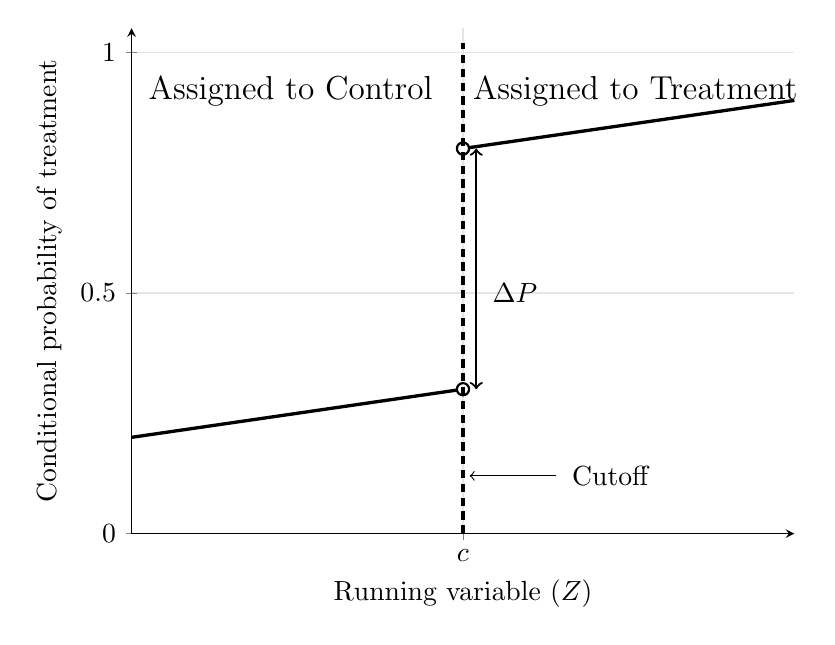
\begin{tikzpicture}
		\begin{axis}[
			width=10cm,height=8cm,
			xmin=-1, xmax=1, ymin=0, ymax=1.05,
			axis lines=left,
			grid=both, grid style={gray!20},
			xlabel={Running variable ($Z$)},
			ylabel={Conditional probability of treatment},
			xtick={0}, xticklabels={$c$},
			ytick={0,0.5,1},
			clip=false
			]
			% Fuzzy RD: probabilities below/above cutoff
			\addplot[very thick] coordinates {(-1,0.20) (0,0.30)};  % left limit p^-
			\addplot[very thick] coordinates {(0,0.80) (1,0.90)};   % right limit p^+
			
			% Open circles at the jump (left/right limits at c)
			\draw[thick, fill=white] (axis cs:0,0.30) circle (2.2pt);
			\draw[thick, fill=white] (axis cs:0,0.80) circle (2.2pt);
			
			% Cutoff (vertical dashed line)
			\addplot[black, densely dashed, very thick] coordinates {(0,0) (0,1.02)};
			
			% Labels for regions
			\node[black] at (axis cs:-0.52,0.92) {\large Assigned to Control};
			\node[black] at (axis cs: 0.52,0.92) {\large Assigned to Treatment};
			
			% Arrow and text to mark "Cutoff"
			\draw[->] (axis cs:0.28,0.12) -- (axis cs:0.02,0.12);
			\node[anchor=west] at (axis cs:0.30,0.12) {Cutoff};
			
			% Bracket showing jump size (optional)
			\draw[<->, thick] (axis cs:0.04,0.30) -- (axis cs:0.04,0.80);
			\node[anchor=west] at (axis cs:0.06,0.50) {$\Delta P$};
			
		\end{axis}
	\end{tikzpicture}
	\caption{Fuzzy regression discontinuity design: Conditional probability of treatment}
	\label{Fig:FRDD}
\end{figure}

Note that the expected value of the observed outcome given the running variable is given by
\begin{align*}
	\mathbb{E}[Y_i\mid Z_i=z]&=\mathbb{E}[Y_i(0)\mid D_i=0, Z_i=z]P(D_i=0\mid Z_i=z)\\
	&+\mathbb{E}[Y_i(1)\mid D_i=1, Z_i=z]P(D_i=1\mid Z_i=z).
\end{align*}

Thus, the observed outcome is a weighted average of potential outcomes. Figure \ref{fig:FRD-muplus-muminus} displays the treatment effect that we are targeting.

\begin{figure}[ht]
	\centering
	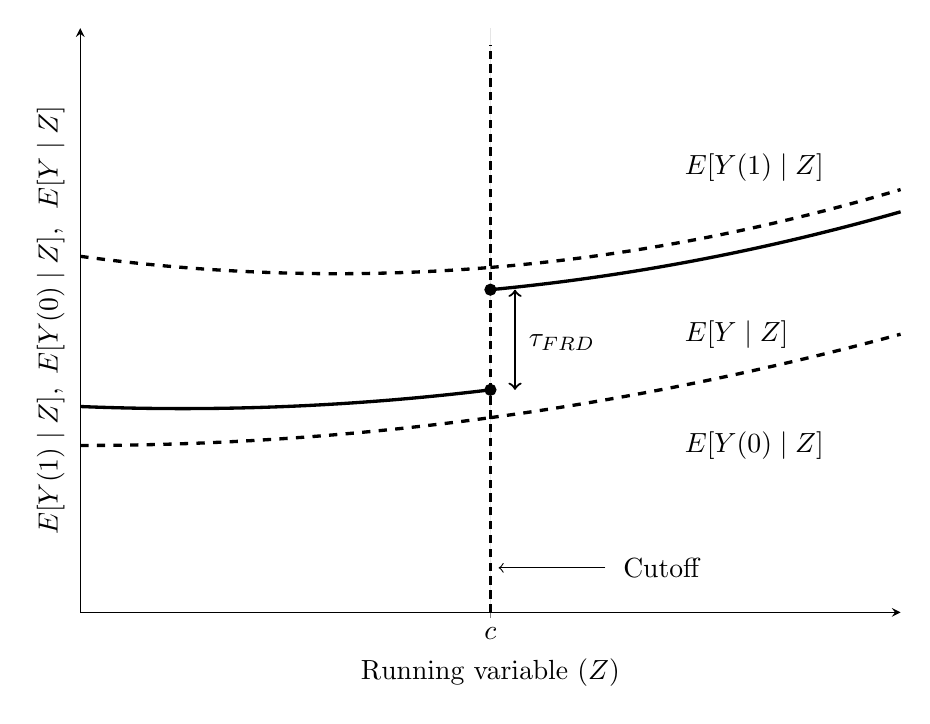
\begin{tikzpicture}
		\begin{axis}[
			width=12cm,height=9cm,
			xmin=-1, xmax=1, ymin=0, ymax=1.05,
			axis lines=left,
			grid=both, grid style={gray!20},
			xlabel={Running variable ($Z$)},
			ylabel={$\mathbb{E}[Y(1)\mid Z],\ \mathbb{E}[Y(0)\mid Z]$, \ $\mathbb{E}[Y\mid Z]$},
			xtick={0}, xticklabels={$c$},
			ytick=\empty,
			clip=false
			]
			
			% --- Choose smooth functions for illustration ---
			% E[Y(0)|X]: observed (solid) for X<c, counterfactual (dashed) for X>=c
			\addplot[black, very thick, dashed, domain=-1:0, samples=200] {0.35 + 0.1*x + 0.05*x^2};
			\addplot[black, very thick, dashed, domain=0:1, samples=200] {0.35 + 0.1*x + 0.05*x^2};
			
			% E[Y(1)|X]: counterfactual (dashed) for X<c, observed (solid) for X>=c
			\addplot[black, very thick, dashed, domain=-1:0, samples=200] {0.62 + 0.06*x + 0.08*x^2};
			\addplot[black, very thick, dashed, domain=0:1, samples=200] {0.62 + 0.06*x + 0.08*x^2};
			
			% E[Y(1)|X]: counterfactual (dashed) for X<c, observed (solid) for X>=c
			\addplot[black, very thick, domain=-1:0, samples=200] {0.4 + 0.09*x + 0.06*x^2};
			\addplot[black, very thick, domain=0:1, samples=200] {0.58 + 0.07*x + 0.07*x^2};
			
			% --- Cutoff (vertical dashed line) ---
			\addplot[black, densely dashed, very thick] coordinates {(0,0) (0,1.02)};
			
			% --- Points at the cutoff (mu_- and mu_+) ---
			\filldraw[black] (axis cs:0,0.4) circle (2pt);  % mu_-
			\filldraw[black] (axis cs:0,0.58) circle (2pt);  % mu_+
			
			% Labels mu_- and mu_+
			% \node[anchor=east] at (axis cs:-0.02,0.35) {$\mu_-$};
			% \node[anchor=east] at (axis cs:-0.02,0.62) {$\mu_+$};
			
			% --- Jump size tau_SRD ---
			\draw[<->, thick] (axis cs:0.06,0.4) -- (axis cs:0.06,0.58);
			\node[anchor=west] at (axis cs:0.07,0.485) {$\tau_{\text{FRD}}$};
			
			% --- Arrow + label "Cutoff" ---
			\draw[->] (axis cs:0.28,0.08) -- (axis cs:0.02,0.08);
			\node[anchor=west] at (axis cs:0.30,0.08) {Cutoff};
			
			% --- Curve labels ---
			\node[black, anchor=west]  at (axis cs:0.45,0.80) {$\mathbb{E}[Y(1)\mid Z]$};
			\node[black, anchor=west] at (axis cs:0.45,0.30) {$\mathbb{E}[Y(0)\mid Z]$};
			\node[black, anchor=west] at (axis cs:0.45,0.50) {$\mathbb{E}[Y\mid Z]$};
			
		\end{axis}
	\end{tikzpicture}
	\caption{RD treatment effect in a fuzzy RD design. Solid segments are observed on each side of $c$; dashed segments are counterfactual.}
	\label{fig:FRD-muplus-muminus}
\end{figure}

The target causal effect in the FRD is (see \cite{hahn2001rdd} for a proof)
\begin{align*}
\tau_{\text{FRD}}
&=
\frac{\lim_{z \downarrow c}\mathbb{E}[Y_i\mid Z_i=z]-\lim_{z \uparrow c}\mathbb{E}[Y_i\mid Z_i=z]}
{\lim_{z \downarrow c}\mathbb{E}[D_i\mid Z_i=z]-\lim_{z \uparrow c}\mathbb{E}[D_i\mid Z_i=z]}\\
&=\mathbb{E}[Y_i(1)-Y_i(0)\mid Z_i=c], \text{units are compliers}.
\end{align*}
Note that $\tau_{\text{FRD}}$ encompasses $\tau_{\text{SRD}}$ as $\lim_{z \downarrow c}\mathbb{E}[D_i\mid Z_i=z]-\lim_{z \uparrow c}\mathbb{E}[D_i\mid Z_i=z]=1$ in the SRD. In addition, $\tau_{\text{FRD}}$ has the same structure as the local average treatment effect (LATE) in the IV literature, with the instrument given by the eligibility indicator \(T_i=\mathbbm{1}\{Z_i\ge c\}\). Because compliance is imperfect (some eligible units do not take treatment and some ineligible units receive it), \(D_i \neq T_i\) for some units, and the estimand pertains to \emph{compliers at the cutoff}.

Let \(D_i(z)\) denote the potential treatment status if the cutoff were \(z\) (for \(z\) in a neighborhood of \(c\)) such that $D_i(z)=1$ implies that the unit would be treated if the cutoff is $z$. The identification assumptions are: 

\textit{1. Continuity of the potential outcome regression functions}, particularly at \(c\).

\textit{2. A nontrivial first stage},
\(\lim_{z \downarrow c}\mathbb{E}[D_i\mid Z_i=z]-\lim_{z \uparrow c}\mathbb{E}[D_i\mid Z_i=z]\neq 0\),

and 

\textit{3. Monotonicity}: \(D_i(z)\) is non-increasing in \(z\) at \(z=c\).

We can classify unit types (locally around the cutoff $c$) using the potential treatment under a hypothetical cutoff $z$, $D_i(z)$ as follows:

\textit{Complier status} \[ \lim_{z\downarrow Z_i}D_i(z)=0, \ \text{and} \ \lim_{z\uparrow Z_i}D_i(z)=1, \]
 
\textit{Never-takers} \[ \lim_{z\downarrow Z_i}D_i(z)=0, \ \text{and} \ \lim_{z\uparrow Z_i}D_i(z)=0, \] 

and
 
\textit{Always-takers} \[ \lim_{z\downarrow Z_i}D_i(z)=1, \ \text{and} \ \lim_{z\uparrow Z_i}D_i(z)=1. \]

Thus, compliers are units that would be treated if the cutoff were at or below their score $Z_i$, and would not be treated if the cutoff were above $Z_i$. Never-takers and always-takers do not change treatment status regardless of the cutoff: the former are always untreated, whereas the latter are always treated. Monotonicity precludes \emph{defiers}.

See \cite{imbens2008regression} and \cite{cattaneo2019practical} for discussions of graphical and formal diagnostics of the assumptions in RD.\\

\textbf{Example: Returns to compulsory schooling \cite{chib2016bayesian}}

\cite{chib2016bayesian} propose a Bayesian inferential framework that explicitly models unit type (complier, always-taker, and never-taker), which enables implementation of a Gibbs sampler. Their empirical application is motivated by the April 1947 reform in the United Kingdom that raised the minimum school-leaving age from 14 to 15.

In the example below, we construct a simulation calibrated to their application to illustrate Bayesian inference in a fuzzy RD. In particular, we specify priors, derive the full conditional distributions, and implement a Gibbs sampler to estimate the treatment effect at the cutoff.

There are three types of individuals: compliers ($c$), never-takers ($n$), and always-takers ($a$). These imply four potential outcomes $Y_{ic}(0)$, $Y_{ic}(1)$, $Y_{in}(0)$, and $Y_{ia}(1)$. \cite{chib2016bayesian} assume
\[
Y_{ic}(0)=\beta_{0c0}+\beta_{0c1}Z_i+\mathbf{X}_i^{\top}\boldsymbol{\beta}_c+\mu_{0ci}=\mathbf{W}_{ic}^{\top}\beta_{0c}+\mu_{0ci},
\]
\[
Y_{ic}(1)=\beta_{1c0}+\beta_{1c1}Z_i+\mathbf{X}_i^{\top}\boldsymbol{\beta}_c+\mu_{1ci}=\mathbf{W}_{ic}^{\top}\beta_{1c}+\mu_{1ci},
\]
\[
Y_{in}(0)=\beta_{n0}+\mathbf{X}_i^{\top}\boldsymbol{\beta}_n+\mu_{ni}=\mathbf{W}_{in}^{\top}\beta_{0n}+\mu_{ni},
\]
and
\[
Y_{ia}(1)=\beta_{a0}+\mathbf{X}_i^{\top}\boldsymbol{\beta}_a+\mu_{ai}=\mathbf{W}_{ia}^{\top}\beta_{1a}+\mu_{ai},
\]
where $\mu_{dci}\sim t_v(0,\sigma^2_{dc})$ for $d\in\{0,1\}$, $\mu_{ni}\sim t_v(0,\sigma^2_{0n})$, and $\mu_{ai}\sim t_v(0,\sigma^2_{1a})$; here $t_v$ denotes the Student-$t$ distribution with $v$ degrees of freedom. The running variable is centered at the cutoff, so $Z_i=0$ at the threshold, and the FRD treatment effect is
\[
\tau_{\text{FRD}}=\beta_{1c0}-\beta_{0c0}.
\]

There are four cells in this setting, defined by policy epochs $\mathbbm{1}(Z_i < 0)$ and $\mathbbm{1}(Z_i \geq 0)$, and treatment values $D_i = 0$ and $D_i = 1$. Table \ref{tab:appCJ} shows the case where, in the cell without treatment under the old policy ($K_{00}$), there are compliers and never-takers, while in the cell with treatment under the new policy ($K_{11}$), there are compliers and always-takers.

\begin{table}[ht]
	\centering
	\caption{Distribution of subject type by observed policy regime and treatment}\label{tab:appCJ}
	\begin{tabular}{lcc}
		\hline
		& \multicolumn{2}{c}{\textbf{Treatment}} \\ 
		\cline{2-3}
		\textbf{Policy indicator} & $D_i = 0$ & $D_i = 1$ \\ 
		\hline
		$\mathbbm{1}(Z_i < 0)$ (old policy) & c, n & a \\
		$\mathbbm{1}(Z_i \geq 0)$ (new policy) & n & c, a \\
		\hline
	\end{tabular}
\end{table}

The four cells by policy and treatment status are:
\[
K_{00} = \{c, n\}, \quad K_{10} = \{n\}, \quad K_{01} = \{a\}, \quad K_{11} = \{c, a\},
\]
and the two cells by treatment status are:
\[
K_0 = \{c, n\}, \quad K_1 = \{c, a\}.
\]

Under a Bayesian framework, posterior simulation simplifies because we sample each unit’s latent type $C_i \in \{c, n, a\}$. This contrasts with the Frequentist literature, where types are not modeled explicitly. Thus, the Bayesian approach requires setting assumptions about the types (see \cite{chib2016bayesian} for details); for instance, types may be distributed smoothly around the cutoff with unknown distributions. In addition, given monotonicity, there are models for four potential outcomes. This differs from the Frequentist literature, which considers only two potential outcomes, given the binary treatment, and a model for the treatment.

Note that if we observe $Z_i < 0$ and $D_i = 0$, only compliers and never-takers are possible. Then,
\[
P(C_i = c \mid Y_i, D_i = 0, \boldsymbol{\theta})
= \frac{\eta_{c} \, t_v\!\big(Y_i \mid \mathbf{W}_{ic}^{\top} \boldsymbol{\beta}_{0c}, \sigma^2_{0c} \big)}
{\eta_{c} \, t_v\!\big(Y_i \mid \mathbf{W}_{ic}^{\top} \boldsymbol{\beta}_{0c}, \sigma^2_{0c} \big) +
	\eta_{n} \, t_v\!\big(Y_i \mid \mathbf{W}_{in}^{\top} \boldsymbol{\beta}_{0n}, \sigma^2_{0n} \big)}, i \in K_{00}
\]
where $\boldsymbol{\theta}$ denotes the set of model parameters, and $\eta_{c}$ and $\eta_{n}$ are the current mixture weights for a complier and a never-taker, respectively.

Conversely, if $Z_i \geq 0$ and $D_i = 1$, only compliers and always-takers are possible:
\[
P(C_i = c \mid Y_i, D_i = 1, \boldsymbol{\theta})
= \frac{\eta_{c} \, t_v\!\big(Y_i \mid \mathbf{W}_{ic}^{\top} \boldsymbol{\beta}_{1c}, \sigma^2_{1c} \big)}
{\eta_{c} \, t_v\!\big(Y_i \mid \mathbf{W}_{ic}^{\top} \boldsymbol{\beta}_{1c}, \sigma^2_{1c} \big) +
	\eta_{a} \, t_v\!\big(Y_i \mid \mathbf{W}_{ia}^{\top} \boldsymbol{\beta}_{1a}, \sigma^2_{1a} \big)}, i \in K_{11}
\]
where $\eta_{a}$ is the mixture weight for an always-taker.

Following \cite{chib2016bayesian}, we assume a Dirichlet prior for the mixing probabilities ($\eta_c, \eta_n,\eta_a$) with hyperparameters $\alpha_{0k}$, $k \in \{c, n, a\}$. The posterior distribution is then Dirichlet with parameters $\alpha_{0k} + \sum_{i=1}^N \mathbbm{1}(C_i = k)$.

In addition, \cite{chib2016bayesian} use the normal--gamma mixture representation of the Student-$t$ distribution, where the mixing parameter satisfies $\lambda_i \sim G(v/2, v/2)$. Consequently, the posterior distribution of $\lambda_i$ is gamma with parameters $(v+1)/2$ and $(v + \sigma_{dk}^{-2}(y_i - \mathbf{W}_{ik}^{\top} \boldsymbol{\beta}_{dk})^2) / 2$.

The prior distribution for the location parameters $\boldsymbol{\beta}_{dk}$ is independent normal with mean $\boldsymbol{\beta}_{dk,0}$ and variance matrix $\mathbf{B}_{dk,0}$. The posterior distribution of $\boldsymbol{\beta}_{dk}$ is normal with mean
\[
\boldsymbol{\beta}_{dk,n} = \mathbf{B}_{dk,n} \left( \mathbf{B}_{dk,0}^{-1} \boldsymbol{\beta}_{dk,0} + \sigma_{dk}^{-2} \sum_{i \in I_{dk}} \lambda_i \mathbf{W}_{ik} Y_i \right),
\]
and covariance matrix
\[
\mathbf{B}_{dk,n} = \left( \mathbf{B}_{dk,0}^{-1} + \sigma_{dk}^{-2} \sum_{i \in I_{dk}} \lambda_i \mathbf{W}_{ik} \mathbf{W}_{ik}^{\top} \right)^{-1},
\]
where $I_{dk} = \{i : D_i = d, C_i = k\}$ is the set of indices for observations by treatment status and unit type. Note that there are only four possible combinations determined by policy and treatment status, namely, $I_{0c}$, $I_{1c}$, $I_{0n}$ and $I_{1a}$.

Finally, assuming that the prior distributions of the variances are independent inverse-gamma, $\sigma_{dk}^2 \sim IG(\alpha_{dk,0}/2, \delta_{dk,0}/2)$, the posterior distributions are also inverse-gamma, $\sigma_{dk}^2 \sim IG(\alpha_{dk,n}/2, \delta_{dk,n}/2)$, where
\[
\alpha_{dk,n} = \alpha_{dk,0} + N_{dk},
\]
and
\[
\delta_{dk,n} = \delta_{dk,0} + \sum_{i \in I_{dk}} \lambda_i \left(Y_i - \mathbf{w}_{ik}^{\top} \boldsymbol{\beta}_{dk} \right)^2.
\]
Here, $N_{dk}$ denotes the number of elements (cardinality) of $I_{dk}$.

The following code performs a simulation assuming that $Z_i$ follows a discrete uniform distribution from $-24$ to $24$, where the policy indicator equals one if $Z_i \geq 0$. Next, $X_i$ follows a discrete uniform distribution between $85$ and $95$. We set $\boldsymbol{\beta}_{0c} = [4.50 \ -0.20 \ 0.03]^{\top}$ and $\boldsymbol{\beta}_{1c} = [5.50 \ 0.40 \ 0.03]^{\top}$, so that the treatment effect is $1$. In addition, $\boldsymbol{\beta}_{0n} = [6.80 \ -0.02]^{\top}$ and $\boldsymbol{\beta}_{1a} = [5.50 \ -0.04]^{\top}$, with $\sigma_{0c}^2 = \sigma_{1c}^2 = 0.10$, $\sigma_{0n}^2 = 0.15$, and $\sigma_{1a}^2 = 0.20$. The type probabilities are $\eta_{c} = 0.70$, $\eta_{n} = 0.15$, and $\eta_{a} = 0.15$. We set the sample size to $3{,}000$ and $v = 5$. In addition, we set non-informative priors, a burn-in of 1,000, and 5,000 MCMC iterations. The following code illustrates the implementation, and Figure \ref{fig12_FRD} presents the posterior distribution of the LATE. The 95\% credible interval encompasses the population value, and the posterior mean lies close to this value.

\begin{tcolorbox}[enhanced,width=4.67in,center upper,
	fontupper=\large\bfseries,drop shadow southwest,sharp corners]
	\textit{R code. Simulation: Fuzzy regression discontinuity design}
	\begin{VF}
		\begin{lstlisting}[language=R]		
rm(list = ls()); set.seed(10101)
# Simulation setup
N <- 3000
Zi <- sample(seq(-24, 24, 1), N, replace = TRUE) # Running var
Z <- Zi - mean(Zi)
T <- as.integer(Z >= 0)                          # Policy (0/1)
X <- sample(seq(85, 95, 1), N, replace = TRUE)   # Regressor
Wc <- cbind(1, Z, X)                             # Compliers
W  <- cbind(1, X)                                # No compliers

B0c <- c(4.5, -0.2, 0.03); B1c <- c(5.5, 0.4,  0.03)
B0n <- c(6.8,  -0.02); B1a <- c(5.5,  -0.04)
s2c <- 0.1; s2n <- 0.15; s2a <- 0.2
Etac <- 0.7; Etan <- 0.15; Etaa <- 0.15
v <- 5
# Potential outcomes (Student-t noise scaled to match variances)
mu0c <- sqrt(s2c) * rt(N, v);  Y0c <- as.numeric(Wc %*% B0c + mu0c)
mu1c <- sqrt(s2c) * rt(N, v);  Y1c <- as.numeric(Wc %*% B1c + mu1c)
mu0n <- sqrt(s2n) * rt(N, v);  Y0n <- as.numeric(W  %*% B0n + mu0n)
mu1a <- sqrt(s2a) * rt(N, v);  Y1a <- as.numeric(W  %*% B1a + mu1a)
# Latent types: first n, then a, remaining are c
id    <- seq_len(N)
n_n   <- as.integer(round(Etan * N))
n_a   <- as.integer(round(Etaa * N))
id0n  <- sample(id, n_n, replace = FALSE)     # never-takers
id_rem <- setdiff(id, id0n)
id1a  <- sample(id_rem, n_a, replace = FALSE) # always-takers
idc   <- setdiff(id, c(id0n, id1a))           # compliers
type <- rep(NA_character_, N)
type[id0n] <- "n"
type[id1a] <- "a"
type[idc]  <- "c"
# Realized treatment under monotonicity:
# n -> D=0, a -> D=1, c -> D=T
D <- integer(N)
D[type == "n"] <- 0; D[type == "a"] <- 1
D[type == "c"] <- T[type == "c"]

# 2x2 table of D vs T
tab_DT <- table(T = factor(T, levels = 0:1), D = factor(D, levels = 0:1))
print(tab_DT)
		\end{lstlisting}
	\end{VF}
\end{tcolorbox}  

\begin{tcolorbox}[enhanced,width=4.67in,center upper,
	fontupper=\large\bfseries,drop shadow southwest,sharp corners]
	\textit{R code. Simulation: Fuzzy regression discontinuity design}
	\begin{VF}
		\begin{lstlisting}[language=R]	
Y <- ifelse(type == "n", Y0n, ifelse(type == "a", Y1a, ifelse(D == 0, Y0c, Y1c)))
## Gibbs sampler ##
I00 <- which(T == 0 & D == 0); I11 <- which(T == 1 & D == 1)
I01 <- which(T == 0 & D == 1); I10 <- which(T == 1 & D == 0)
# Hyperparameters
a0c <- 1; a0n <- 1; a0a <- 1 # Hyperpar Dirichlet
v <- 5 # Student-t
a0 <- 0.01; d0 <- 0.01 # Inv-Gamma
# Prob complier | D=0
dens_t_locscale <- function(y, mu, sig2, v) {
	z <- (y - mu) / sqrt(sig2); dt(z, df = v) / sqrt(sig2)
}
Pc0 <- function(b0c, sigma20c, etac, b0n, sigma20n, etan, i){
	p0c <- etac * dens_t_locscale(Y[i], mu = sum(Wc[i,]*b0c), sig2 = sigma20c, v = v)
	p0n <- etan * dens_t_locscale(Y[i], mu = sum(W[i, ]*b0n), sig2 = sigma20n, v = v)
	pc0 <- p0c / (p0c + p0n + 1e-12)
	return(pc0)
}
Pc1 <- function(b1c, sigma21c, etac, b1a, sigma21a, etaa, i){
	p1c <- etac * dens_t_locscale(Y[i], mu = sum(Wc[i,]*b1c), sig2 = sigma21c, v = v)
	p1a <- etaa * dens_t_locscale(Y[i], mu = sum(W[i, ]*b1a), sig2 = sigma21a, v = v)
	pc1 <- p1c / (p1c + p1a + 1e-12)
	return(pc1)
}
rtype <- function(alphas){
	types <- MCMCpack::rdirichlet(1, alphas)
	return(types)
}
PostLambda_i <- function(sig2, Beta, yi, hi, v){
	shape <- (v + 1)/2
	rate  <- (v + (yi - sum(hi * Beta))^2 / sig2)/2
	rgamma(1, shape = shape, rate = rate)
}
PostBeta <- function(sig2, lambda, y, H){
	k <- dim(H)[2]; B0i <- solve(1000*diag(k))
	b0 <- rep(0, k)
	Bn <- solve(B0i + sig2^(-1)*t(H)%*%diag(lambda)%*%H)
	bn <- Bn%*%(B0i%*%b0 + sig2^(-1)*t(H)%*%diag(lambda)%*%y)
	Beta <- MASS::mvrnorm(1, bn, Bn)
	return(Beta)
}
PostSig2 <- function(Beta, lambda, y, H){
	Ndk <- length(y); an <- a0 + Ndk 
	dn <- d0 + t(y - H%*%Beta)%*%diag(lambda)%*%(y - H%*%Beta)
	sig2 <- invgamma::rinvgamma(1, shape = an/2, rate = dn/2)
	return(sig2)
}
\end{lstlisting}
	\end{VF}
\end{tcolorbox}  

\begin{tcolorbox}[enhanced,width=4.67in,center upper,
	fontupper=\large\bfseries,drop shadow southwest,sharp corners]
	\textit{R code. Simulation: Fuzzy regression discontinuity design}
	\begin{VF}
		\begin{lstlisting}[language=R]	
# MCMC parameter
burnin <- 1000; S <- 5000; tot <- S + burnin 
ETAs <- matrix(NA, tot, 3)
BETAS0C <- matrix(NA, tot, 3); BETAS1C <- matrix(NA, tot, 3)
BETASA <- matrix(NA, tot, 2); BETASN <- matrix(NA, tot, 2)
SIGMAS <- matrix(NA, tot, 4)
b0c <- rep(0, 3); b1c <- rep(0, 3); b1a <- rep(0, 2); b0n <- rep(0, 2)
sigma21c <- 0.1; sigma20c <- 0.1; sigma20n <- 0.1; sigma21a <- 0.1
EtacNew <- 0.5; EtanNew <- 0.25; EtaaNew <- 0.25
pb <- txtProgressBar(min = 0, max = tot, style = 3)
for(s in 1:tot){
	ProbC0 <- sapply(I00, function(i)Pc0(b0c, sigma20c, EtacNew, b0n, sigma20n, EtanNew, i = i))
	ProbC1 <- sapply(I11, function(i)Pc1(b1c, sigma21c, EtacNew, b1a, sigma21a, EtaaNew, i = i))
	Typec0 <- sapply(ProbC0, function(p) {sample(c("c", "n"), 1, prob = c(p, 1-p))})
	Typec1 <- sapply(ProbC1, function(p) {sample(c("c", "a"), 1, prob = c(p, 1-p))})
	typeNew <- rep(NA_character_, N)
	typeNew[I10] <- "n"; typeNew[I01] <- "a"
	typeNew[I00]  <- Typec0; typeNew[I11]  <- Typec1
	Nc <- sum(typeNew == "c"); Na <- sum(typeNew == "a")
	Nn <- sum(typeNew == "n");
	anc <- a0c + Nc; ann <- a0n + Nn; ana <- a0a + Na
	alphas <- c(anc, ann, ana)
	EtasNew <- rtype(alphas = alphas)
	EtacNew <- EtasNew[1]; EtanNew <- EtasNew[2]
	EtaaNew <- EtasNew[3]
	ETAs[s, ] <- EtasNew; Lambda <- numeric(N)
	idx_n <- which(typeNew == "n")
	idx_a <- which(typeNew == "a")
	idx_c0 <- which(typeNew == "c" & D == 0); idx_c1 <- which(typeNew == "c" & D == 1)
	Lambda[idx_n]  <- sapply(idx_n,  function(i) PostLambda_i(sigma20n, b0n, Y[i],  W[i, ], v))
	Lambda[idx_a]  <- sapply(idx_a,  function(i) PostLambda_i(sigma21a, b1a, Y[i],  W[i, ], v))
	Lambda[idx_c0] <- sapply(idx_c0, function(i) PostLambda_i(sigma20c, b0c, Y[i], Wc[i, ], v))
	Lambda[idx_c1] <- sapply(idx_c1, function(i) PostLambda_i(sigma21c, b1c, Y[i], Wc[i, ], v))
	b1a <- PostBeta(sig2 = sigma21a, lambda = Lambda[idx_a], y = Y[idx_a], H = W[idx_a,])
	b0n <- PostBeta(sig2 = sigma20n, lambda = Lambda[idx_n], y = Y[idx_n], H = W[idx_n,])
	b0c <- PostBeta(sig2 = sigma20c, lambda = Lambda[idx_c0], y = Y[idx_c0], H = Wc[idx_c0,])
	b1c <- PostBeta(sig2 = sigma21c, lambda = Lambda[idx_c1], y = Y[idx_c1], H = Wc[idx_c1,])
	BETASA[s, ] <- b1a; BETASN[s, ] <- b0n
	BETAS0C[s, ] <- b0c; BETAS1C[s, ] <- b1c 
\end{lstlisting}
	\end{VF}
\end{tcolorbox}  

\begin{tcolorbox}[enhanced,width=4.67in,center upper,
	fontupper=\large\bfseries,drop shadow southwest,sharp corners]
	\textit{R code. Simulation: Fuzzy regression discontinuity design}
	\begin{VF}
		\begin{lstlisting}[language=R]	
	sigma21a <- PostSig2(Beta = b1a, lambda = Lambda[idx_a], y = Y[idx_a], H = W[idx_a,])
	sigma20n <- PostSig2(Beta = b0n, lambda = Lambda[idx_n], y = Y[idx_n], H = W[idx_n,])
	sigma20c <- PostSig2(Beta = b0c, lambda = Lambda[idx_c0], y = Y[idx_c0], H = Wc[idx_c0,])
	sigma21c <- PostSig2(Beta = b1c, lambda = Lambda[idx_c1], y = Y[idx_c1], H = Wc[idx_c1,])
	SIGMAS[s, ] <- c(sigma21a, sigma20n, sigma20c, sigma21c)
	setTxtProgressBar(pb, s)
}
close(pb)
keep <- seq((burnin+1), tot)
LATE <- coda::mcmc(BETAS1C[keep, 1] - BETAS0C[keep, 1])
# Extract samples as numeric
late_draws <- as.numeric(LATE)
# Posterior mean and 95% CI
LATEmean <- mean(late_draws)
LATEci   <- quantile(late_draws, c(0.025, 0.975))
# Plot posterior density
df <- data.frame(LATE = late_draws)

ggplot(df, aes(x = LATE)) + geom_density(fill = "skyblue", alpha = 0.5, color = "blue") + geom_vline(xintercept = LATEmean, color = "red", linetype = "dashed", linewidth = 1) + geom_vline(xintercept = LATEci, color = "black", linetype = "dotted", linewidth = 1) + labs(title = "Posterior distribution of LATE",
subtitle = paste0("Mean = ", round(LATEmean,3), " | 95% CI = [", round(LATEci[1],3), ", ", round(LATEci[2],3), "]"), x = "LATE", y = "Density") +
theme_bw(base_size = 14)
		\end{lstlisting}
	\end{VF}
\end{tcolorbox}  

\begin{figure}[h!]
	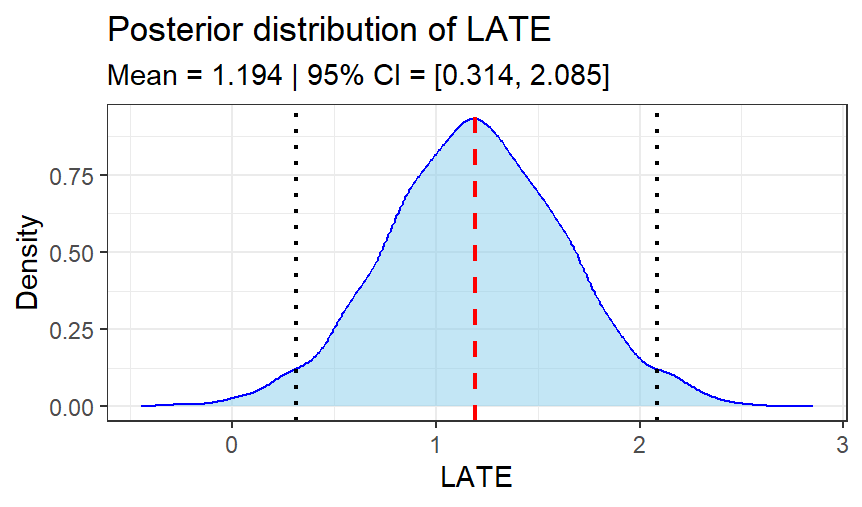
\includegraphics[width=340pt, height=200pt]{Chapters/chapter12/figures/FigFRD.png}
	\caption[List of figure caption goes here]{Posterior distribution of LATE: Simulation of fuzzy regression discontinuity design}\label{fig12_FRD}
\end{figure}


A difference in this example is that, unlike most of the Frequentist literature, the entire dataset on the forcing variable is used. \cite{chib2023nonparametric} propose a non-parametric Bayesian framework that emphasizes the data near the cutoff using a \textit{soft-window} approach. Other Bayesian approaches to inference in RD include \cite{branson2019nonparametric}, who use Gaussian process regression to model the conditional expectation function, and \cite{rischard2020bayesian}, who develop a non-parametric Bayesian framework for spatial RD.

\section{Sample selection}\label{sec12_8}

In Figure \ref{DAG3} in Section \ref{chap12_3}, we depict a situation of collider bias that induces selection bias. Specifically, conditioning on a particular subset of the population ($D_i=1$), where $D_i$ is influenced by both the treatment and confounders, opens a back-door path and creates a spurious association between their causes. Placing this situation within the well-known sample selection framework \cite{heckman1979sample}, the observed outcome can be represented as
\begin{align*}
	Y_i = \begin{cases}
		Y_i(1) & \text{if } D_i=1, \\
		\text{NA} & \text{if } D_i=0,
	\end{cases}
\end{align*}
that is, we only observe $Y_i = Y_i(1)$ for $i=1,2,\dots,N$, while $Y_i(0)$ remains unobserved (``missing'').

In this setting, inference can be performed based on the likelihood of the observed outcomes together with the \textit{selection (missingness) mechanism} $(Y_i(1),D_i)$, integrating out the unobserved $Y_i(0)$ from the joint distribution of $\{Y_i(1),Y_i(0),D_i\}$. However, one must consider whether the missingness mechanism is \textit{ignorable} or not. According to \cite{little2019statistical}, the missingness mechanism is ignorable in Bayesian inference if the following two conditions hold:  
i) the likelihood can be factorized as
\[
p(y_i, d_i\mid \boldsymbol{\theta},\boldsymbol{\gamma}) 
= p(y_i\mid \boldsymbol{\theta})\, p(y_i,d_i \mid \boldsymbol{\gamma}),
\] 
and  
ii) the parameters $\boldsymbol{\theta}$ and $\boldsymbol{\gamma}$ are \emph{a priori} independent,
\[
\pi(\boldsymbol{\theta},\boldsymbol{\gamma}) 
= \pi(\boldsymbol{\theta})\,\pi(\boldsymbol{\gamma}).
\]

Under these conditions, posterior inference can be based on
\[
\pi(\boldsymbol{\theta}\mid \mathbf{y}) 
\propto \pi(\boldsymbol{\theta})\, p(\mathbf{y} \mid \boldsymbol{\theta}).
\]
Thus, if the missingness mechanism is \textit{Missing At Random} (MAR) and the parameters are \emph{a priori} independent, the missingness mechanism is ignorable for Bayesian inference (see Chapter~6 of \cite{little2019statistical}).

In contrast, when the missingness mechanism is non-ignorable (i.e., Not Missing At Random, NMAR), the probability of observing $Y_i$ depends on the unobserved values themselves. In this case, Bayesian inference must be performed using the full joint likelihood,
\[
p(y_i, d_i \mid \boldsymbol{\theta},\boldsymbol{\gamma}),
\]
which requires specifying and estimating both the outcome model and the selection model simultaneously (see Chapter~15 of \cite{little2019statistical}). In particular, the classical sample selection model of \cite{heckman1979sample} establishes,
\begin{align*}
	Y_i = \begin{cases}
		\mathbf{X}_i^{\top}\boldsymbol{\beta}+\mu_i & \text{if } D_i=1, \\
		\text{NA} & \text{if } D_i=0,
	\end{cases}
\end{align*}

\begin{align*}
	D_i = \begin{cases}
		1 & \text{if } D_i^* = \mathbf{Z}_i^{\top}\boldsymbol{\gamma}+\nu_i > 0, \\
		0 & \text{if } D_i^* = \mathbf{Z}_i^{\top}\boldsymbol{\gamma}+\nu_i \leq 0,
	\end{cases}
\end{align*}

where
\begin{align}
	\begin{bmatrix}
		\mu_i \\[6pt]
		\nu_i
	\end{bmatrix}
	\sim N\!\left(
	\begin{bmatrix}
		0 \\ 0
	\end{bmatrix},
	\begin{bmatrix}
		\sigma^2_{\mu} & \sigma_{\mu\nu} \\
		\sigma_{\mu\nu} & 1
	\end{bmatrix}\right).
\end{align}
The restriction $\operatorname{Var}(\nu_i)=1$ is imposed for identification. 
Without this normalization, the latent index $D_i^*=\mathbf{Z}_i^{\top}\boldsymbol{\gamma}+\nu_i$ is only identified up to scale, since
\[
P(D_i=1) = P(\mathbf{Z}_i^{\top}\boldsymbol{\gamma}+\nu_i > 0) 
= P\!\left(\frac{\nu_i}{c} > -\frac{\mathbf{Z}_i^{\top}\boldsymbol{\gamma}}{c}\right),
\quad \forall\, c>0.
\]
Thus, setting $\sigma^2_{\nu}=1$ yields point identification of the parameters.

Note that since \(D_i=1 \iff \nu_i>-\mathbf Z_i^\top\boldsymbol\gamma\),
\[
\mathbb E[\mu_i\mid D_i=1,\mathbf Z_i]
=\mathbb E\!\big[\mathbb E(\mu_i\mid \nu_i)\,\big|\,\nu_i>-\mathbf Z_i^\top\boldsymbol\gamma\big]
=\sigma_{\mu\nu}\,\mathbb E\!\big[\nu_i\mid \nu_i>-\mathbf Z_i^\top\boldsymbol\gamma\big].
\] This is because $\mu_i\mid \nu_i\sim N(\sigma_{\mu\nu}\nu_i, \sigma^2_{\mu}-\sigma_{\mu\nu}^2)$.

If \(\nu\sim\mathcal N(0,1)\), then for \(a=\mathbf Z_i^\top\boldsymbol\gamma\),
\[
\mathbb E[\nu\mid \nu>-a]=\frac{\phi(a)}{\Phi(a)}\equiv \lambda(a),
\]
where \(\phi\) and \(\Phi\) are the standard normal pdf and cdf. Hence
\[
\mathbb E[\mu_i\mid D_i=1,\mathbf Z_i]=\sigma_{\mu\nu}\,\lambda(\mathbf Z_i^\top\boldsymbol\gamma)
	=\rho\,\sigma_\mu\,\lambda(\mathbf Z_i^\top\boldsymbol\gamma),
\]
where $\rho=\sigma_{\mu\nu}/\sigma_{\mu}$.

Then, 
\begin{align*}
	\mathbb E[Y_i\mid D_i=1,\mathbf X_i,\mathbf Z_i]
	&=\mathbf X_i^\top \boldsymbol\beta+\mathbb E[\mu_i\mid D_i=1,\mathbf Z_i]\\
	&=\mathbf X_i^\top \boldsymbol\beta + \sigma_{\mu\nu}\,\lambda(\mathbf Z_i^\top\boldsymbol\gamma)\\
	&=\mathbf X_i^\top \boldsymbol\beta + \rho\,\sigma_\mu\,\lambda(\mathbf Z_i^\top\boldsymbol\gamma).
\end{align*}

This is the Heckman selection-bias correction: the inverse Mills ratio \(\lambda(\mathbf Z_i^\top\boldsymbol\gamma)\) enters as an additional regressor in the selected sample.
Point identification can be achieved through functional form (since the inverse Mills ratio is non-linear) together with the normality assumption. This implies that, in principle, one may have $\mathbf{X}_i=\mathbf{Z}_i$. However, such identification is weak, and it is preferable to include at least one variable in $\mathbf{Z}_i$ that is excluded from $\mathbf{X}_i$, i.e., $\mathbf{X}_i\neq\mathbf{Z}_i$, as this strengthens identification and also improves the precision of inference.

To perform Bayesian inference in this model, we use the augmented likelihood. Thus,
\begin{align*}
	\pi(\boldsymbol{\delta},\sigma^2_{\mu},\sigma_{\mu\nu},D_i^*\mid \mathbf{y},\mathbf{d}) 
	& \propto \prod_{i\in I_{0}} \pi(D_i^*\mid \boldsymbol{\delta},\sigma^2_{\mu},\sigma_{\mu\nu}) 
	\, \mathbbm{1}(d_i=0)\, \mathbbm{1}(D_i^*\leq 0) \\
	& \quad \times \prod_{i\in I_{1}} p(y_i,D_i^*\mid \boldsymbol{\delta},\sigma^2_{\mu},\sigma_{\mu\nu}) 
	\, \mathbbm{1}(d_i=1)\, \mathbbm{1}(D_i^*> 0) \\
	& \quad \times \pi(\boldsymbol{\delta},\sigma^2_{\mu},\sigma_{\mu\nu}),
\end{align*}
where $\boldsymbol{\delta}=[\boldsymbol{\beta}^{\top} \ \boldsymbol{\gamma}^{\top}]^{\top}$, 
$I_0=\{i : d_i=0\}$ and $I_1=\{i : d_i=1\}$.

Following Chapter~11 in \cite{greenberg2012introduction}, we set
\[
\boldsymbol{\eta}_i=
\begin{cases}
	[0, \, D_i^*]^{\top}, & i\in I_0\\
	[y_i, \, D_i^*]^{\top}, & i\in I_1
\end{cases},
\qquad
\mathbf{W}_i=\begin{bmatrix}
	\mathbf{X}_i^{\top} & \mathbf{0}\\
	\mathbf{0} & \mathbf{Z}_i^{\top}
\end{bmatrix}, 
\qquad
\mathbf{J}=\begin{bmatrix}
	0 & 0\\
	0 & 1
\end{bmatrix}.
\]

Assuming $\pi(\boldsymbol{\delta}) \sim N(\boldsymbol{\delta}_0,\mathbf{D}_0)$, the conditional posterior distribution of $\boldsymbol{\delta}$ is normal with mean
\[
\boldsymbol{\delta}_n=\mathbf{D}_n\left[\sum_{i\in I_0}\mathbf{W}_i^{\top}\mathbf{J}\boldsymbol{\eta}_i
+\sum_{i\in I_1}\mathbf{W}_i^{\top}\boldsymbol{\Sigma}^{-1}\boldsymbol{\eta}_i
+\mathbf{D}_0^{-1}\boldsymbol{\delta}_0\right],
\]
and variance matrix
\[
\mathbf{D}_n=\left[\sum_{i\in I_0}\mathbf{W}_i^{\top}\mathbf{J}\mathbf{W}_i
+\sum_{i\in I_1}\mathbf{W}_i^{\top}\boldsymbol{\Sigma}^{-1}\mathbf{W}_i
+\mathbf{D}_0^{-1}\right]^{-1},
\] 
where 
\[
\boldsymbol{\Sigma}=\begin{bmatrix}
	\sigma^2_{\mu} & \sigma_{\mu\nu} \\[6pt]
	\sigma_{\mu\nu} & 1
\end{bmatrix}.
\]

Let $\omega=\sigma^2_{\mu}-\sigma^2_{\mu\nu}$ denote the conditional variance of $\mu_i \mid \nu_i$. 
Assuming $\omega^{-1}\sim G(\alpha_0/2,\delta_0/2)$ and noting that
\[
p(y_i,D_i^*\mid \boldsymbol{\delta},\omega,\sigma_{\mu\nu})
= p(y_i\mid D_i^*, \boldsymbol{\delta},\omega,\sigma_{\mu\nu})
\times p(D_i^*\mid \boldsymbol{\delta},\omega,\sigma_{\mu\nu}),
\]
the conditional posterior distribution of $\omega^{-1}$ is Gamma,
\[
\omega^{-1}\mid \boldsymbol{\delta},\sigma_{\mu\nu}, \mathbf{y},\mathbf{d} \sim G(\alpha_n/2,\delta_n/2),
\]
with
\[
\alpha_n=\alpha_0+N_1,
\qquad
\delta_n=\delta_0+\sum_{i\in I_1}\Big[y_i-\mathbf{X}_i^{\top}\boldsymbol{\beta}
-\sigma_{\mu\nu}(D_i^*-\mathbf{Z}_i^{\top}\boldsymbol{\gamma})\Big]^2,
\]
where $N_1$ is the number of observations with $D_i=1$.

In addition, assuming $\sigma_{\mu\nu}\sim N(s_0,S_0)$, the conditional posterior distribution is normal with mean
\[
s_n=S_n\left(\omega^{-1}\sum_{i=1}^N(D_i^*-\mathbf{Z}_i^{\top}\boldsymbol{\gamma})(y_i-\mathbf{X}_i^{\top}\boldsymbol{\beta})
+S_0^{-1}s_0\right),
\]
and variance
\[
S_n=\left[\omega^{-1}\sum_{i=1}^N(D_i^*-\mathbf{Z}_i^{\top}\boldsymbol{\gamma})^2+S_0^{-1}\right]^{-1}.
\]

Finally, since
\[
p(y_i,D_i^*\mid \boldsymbol{\delta},\omega,\sigma_{\mu\nu})
= p(D_i^*\mid y_i, \boldsymbol{\delta},\omega,\sigma_{\mu\nu})
\times p(y_i\mid \boldsymbol{\delta},\omega,\sigma_{\mu\nu}),
\]
the conditional posterior distribution of $D_i^*$ is
\[
D_i^* \sim 
\begin{cases}
	TN_{(-\infty,0]}(\mathbf{Z}_i^{\top}\boldsymbol{\gamma},\,1), & i\in I_0,\\[6pt]
	TN_{(0,\infty)}\!\left(\mathbf{Z}_i^{\top}\boldsymbol{\gamma}
	+\dfrac{\sigma_{\mu\nu}}{\sigma_{\mu\nu}^2+\omega}\,(y_i-\mathbf{X}_i^{\top}\boldsymbol{\beta}),\,
	\dfrac{\omega}{\sigma_{\mu\nu}^2+\omega}\right), & i\in I_1,
\end{cases}
\]
where $TN_{A}(\mu,\sigma^2)$ denotes a normal distribution with mean $\mu$ and variance $\sigma^2$, truncated to the set $A$.\\

\textbf{Example: Simulation of the sample selection model}

We simulate the model 
\[
Y_i = 12 + X_{i1} + X_{i2} + \mu_i,
\]
where $X_{i1}\sim N(0,4)$, $X_{i2}\sim \text{Bin}(1,0.5)$, and $\mu_i\sim N(0,1.2)$ for $i=1,2,\dots,1000$.  
In addition, 
\[
D_i^* = 1 + Z_{i1} - X_{i2} + \nu_i,
\]
where $Z_{i1}\sim N(0,4)$.

The covariance between $\mu_i$ and $\nu_i$ is set to $0.6$.

The hyperparameters are $\boldsymbol{\delta}_0=[0 \ 0 \ 0 \ 0 \ 0 \ 0]^{\top}$, $\mathbf{D}_0=1000\mathbf{I}_6$, $\alpha_0=\delta_0=0.001$, $s_0=0$, and $S_0=1000$. We perform 1,500 iterations with a burn-in of 500. The following code illustrates the Gibbs sampler. Finally, we compare the results with an implementation that does not account for the sample selection issue.

Figure \ref{fig12_SEL} shows the posterior distributions of the second parameter in the outcome equation, whose population value is 1 (black dashed line). The posterior distribution of the model that accounts for selection encompasses the population value, whereas the model that ignores selection does not.

\begin{tcolorbox}[enhanced,width=4.67in,center upper,
	fontupper=\large\bfseries,drop shadow southwest,sharp corners]
	\textit{R code. Simulation: Sample selection model}
	\begin{VF}
		\begin{lstlisting}[language=R]	
rm(list = ls()); set.seed(10101)
library(doParallel); library(snow)
N <- 1000
w1 <- rbinom(N, 1, 0.5) # rnorm(N, 0, sigExo); 
delta <- c(1, 1, -1); beta <- c(2,1,1)
zx <- MASS::mvrnorm(N, mu = rep(0, 2), matrix(c(1,0.7,0.7,1),2,2))
z1 <- zx[,1]
Z <- cbind(1, z1, w1)
sig12 <- 0.8; sig11 <- 1.2
SIGMA <- matrix(c(sig11, sig12, sig12, 1), 2, 2)
E <- MASS::mvrnorm(N, mu = rep(0, 2), SIGMA)
cl <- Z%*%delta + E[,2]; c <- cl > 0
x1 <- zx[,2]; X <- cbind(1, x1, w1)
y <- X%*%beta + E[,1]
y[c==0] <- NA
# Hyperparameters
b0 <- rep(0, 6); B0 <- 1000*diag(6); B0i <- solve(B0)
a0 <- 0.001; d0 <- 0.001
s0 <- 0; S0 <- 1000; S0i <- 1/S0
# Location
idc1 <- which(c==1)
nc1 <- length(idc1)
PostThetaNew <- function(Sigma, clat){
	J <- matrix(c(0,0,0,1),2,2)
	WW <- matrix(0, 6, 6)
	Wy <- matrix(0, 6, 1)
	for(i in 1:N){
		if(i %in% idc1){
			yclat <- c(y[i], clat[i])
			Auxi <- solve(Sigma)
		}else{
			yclat <- c(0, clat[i])
			Auxi <- J
		}
		Wi <- as.matrix(Matrix::bdiag(X[i,], Z[i,]))
		WWi <- Wi%*%Auxi%*%t(Wi)
		Wyi <- Wi%*%Auxi%*%yclat
		WW <- WW + WWi
		Wy <- Wy + Wyi
	}
	Bn <- solve(B0i + WW)
	bn <- Bn%*%(B0i%*%b0 + Wy)
	Beta <- MASS::mvrnorm(1, bn, Bn)
	return(Beta)
}
PostOmega11 <- function(theta, sig12, clat){
	an <- a0 + nc1
	mui <- y[idc1] -X[idc1, ]%*%theta[1:3] - sig12*(clat[idc1] - Z[idc1,]%*%theta[4:6])
	dn <- d0 + t(mui)%*%mui
	omega11 <- LaplacesDemon::rinvgamma(1, an/2, dn/2)
	return(omega11)
}
\end{lstlisting}
\end{VF}
\end{tcolorbox}  

\begin{tcolorbox}[enhanced,width=4.67in,center upper,
	fontupper=\large\bfseries,drop shadow southwest,sharp corners]
	\textit{R code. Simulation: Sample selection model}
	\begin{VF}
		\begin{lstlisting}[language=R]	
PostSig12 <- function(omega11, theta, clat){
	Sn <- (omega11^(-1)*sum((clat[idc1] - Z[idc1,]%*%theta[4:6])^2) + S0i)^(-1)
	sn <- Sn*(omega11^(-1)*sum((clat[idc1] - Z[idc1,]%*%theta[4:6])*(y[idc1] - X[idc1,]%*%theta[1:3])) + s0*S0i)
	sig12 <- rnorm(1, sn, sd = Sn^0.5)
	return(sig12)
}
PostClat <- function(theta, sig12, omega11, i){
	if(i %in% idc1){
		mu <- Z[i,]%*%theta[4:6] + (sig12/(omega11+sig12^2))*(y[i] - X[i,]%*%theta[1:3])
		sig2 <- omega11/(omega11+sig12^2)
		clat <- EnvStats::rnormTrunc(1, mean = mu, sd = sig2^0.5, min = 0, max = Inf)
	}else{
		mu <- Z[i,]%*%theta[4:6]
		clat <- EnvStats::rnormTrunc(1, mean = mu, sd = 1, min = -Inf, max = 0)
	}
	return(clat)
}
# Sampler
S <- 1500; burnin <- 500; thin <- 2
keep <- seq(burnin+thin, S, thin)
PostThetasDraws <- matrix(NA, S, 6)
PostSigmaDraws <- matrix(NA, S, 2)
# Initial parameters
Thetap <- rep(0, 6); Sigmap <- diag(2) 
Sig12p <- 0; Omega11p <- 1
for(i in 1:N){
	if(c[i] == 0){
		LatPost <- EnvStats::rnormTrunc(1, mean = 0, sd = 1, min = -Inf, max = 0)
	}else{
		LatPost <- EnvStats::rnormTrunc(1, mean = 0, sd = 1, min = 0, max = Inf)
	}
}
#### Parallel code ####
cn <- detectCores() 
ClusterHope <- makeCluster(cn, type = "SOCK")
registerDoParallel(ClusterHope)
clusterExport(ClusterHope, list("Z", "X", "c", "y", "N", "idc1", "nc1", "PostClat","Thetap", "Sig12p", "Omega11p"))
\end{lstlisting}
	\end{VF}
\end{tcolorbox}  

\begin{tcolorbox}[enhanced,width=4.67in,center upper,
	fontupper=\large\bfseries,drop shadow southwest,sharp corners]
	\textit{R code. Simulation: Sample selection model}
	\begin{VF}
		\begin{lstlisting}[language=R]	
pb <- txtProgressBar(min = 0, max = tot, style = 3)
for(rep in 1:S){
	LatPost <- t(parSapply(ClusterHope, 1:N, function(i){PostClat(theta = Thetap, sig12 = Sig12p, omega11 = Omega11p, i)}))
	Thetap <- PostThetaNew(Sigma = Sigmap, clat = LatPost)
	Omega11p <- PostOmega11(theta = Thetap, sig12 = Sig12p, clat = LatPost)
	Sig12p <- PostSig12(omega11 = Omega11p, theta = Thetap, clat = LatPost)
	Sigmap <- matrix(c(Omega11p+Sig12p^2, Sig12p, Sig12p, 1),2,2)
	PostThetasDraws[rep,] <- Thetap
	PostSigmaDraws[rep, ] <- c(Omega11p+Sig12p^2, Sig12p)
	clusterExport(ClusterHope, list("Thetap", "Sig12p", "Omega11p"))
	setTxtProgressBar(pb, rep)
}
stopCluster(ClusterHope)
close(pb)
thetaHat <- coda::mcmc(PostThetasDraws[keep,])
PostDrawsSigma <- coda::mcmc(PostSigmaDraws[keep,])
summary(thetaHat)
summary(PostDrawsSigma)
RegNOsel <- MCMCpack::MCMCregress(y ~ X - 1)
summary(RegNOsel)
\end{lstlisting}
	\end{VF}
\end{tcolorbox}

\begin{figure}[h!]
	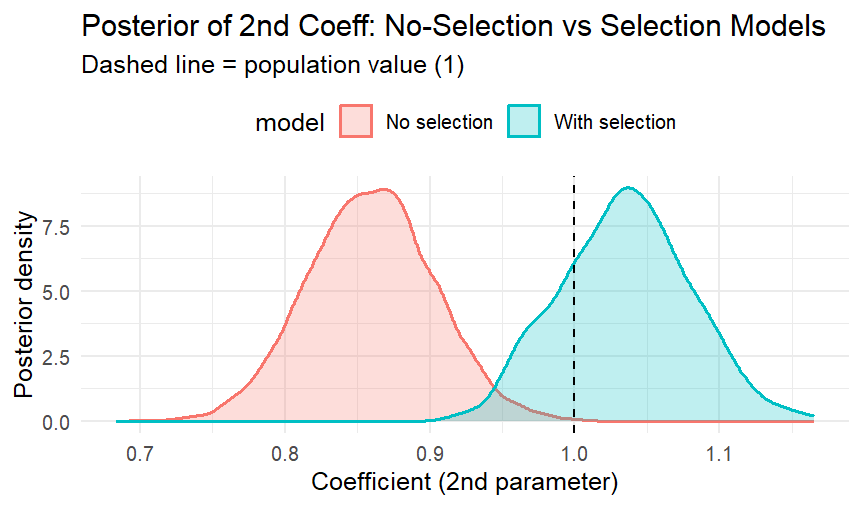
\includegraphics[width=340pt, height=200pt]{Chapters/chapter12/figures/FigSEL.png}
	\caption[List of figure caption goes here]{Posterior distribution second parameter in outcome: Selection vs no selection models}\label{fig12_SEL}
\end{figure}
  
The original Heckman selection model was not intended to calculate the ATE, since $Y_i(0)$ is not observed and, therefore, a treatment effect is not defined. Its main purpose is to correct the expected value of $Y_i \mid D_i=1$ by accounting for sample selection. Subsequently, \cite{heckman1990varieties} and \cite{heckman2005structural} extended the sample selection framework to incorporate $Y_i(0)$, framing the Roy model \cite{roy1951some} within the treatment effect literature and establishing the identification conditions for different treatment parameters. In particular, \cite{heckman2005structural} introduced the marginal treatment effect (MTE),
\[
\tau_{MTE}(x,u_D) = \mathbb{E}[Y_i(1)-Y_i(0)\mid \mathbf{X}_i=\mathbf{x}, \, U_{Di}=u_D],
\]
which is the expected effect of treatment for individuals with observed characteristics $\mathbf{X}_i=\mathbf{x}$ and unobservable factors from the treatment assignment $U_{Di}=u_D$ \cite{heckman2005structural}.

The MTE is a unifying concept that connects the treatment effect, selection, and matching literatures. Moreover, these authors show that many treatment effect parameters, such as the ATE, ATT, and LATE, can be expressed as weighted averages of the MTE (see Table~IA in \cite{heckman2005structural}).

In the Bayesian literature, several authors have estimated different versions of selection models. In particular, \cite{van2011bayesian} and \cite{ding2014bayesian} analyze the sample selection model using flexible specifications for the error terms, while \cite{koop1997learning} and \cite{chib2007analysis} estimate the Roy model. Furthermore, \cite{chib2009estimation} extend the basic framework to a semiparametric setting that accounts for endogeneity, and \cite{heckman2014treatment} introduce latent factors to address the fundamental problem of causal inference in the Roy model. This approach allows researchers to learn about the otherwise unidentified covariance between $Y_i(1)$ and $Y_i(0)$, which in turn enables the estimation of distributional versions of treatment effects that require the joint distribution of $Y_i(1)$ and $Y_i(0)$.

\section{Bayesian exponentially tilted empirical likelihood}\label{sec12_9}

Bayesian parametric approaches are often criticized because they require distributional assumptions that may be arbitrary or remain unchecked. For example, in this chapter we model a continuous outcome as normally distributed. This choice is defensible: among all distributions with a fixed mean and variance, the normal imposes the least prior structure (it maximizes entropy; see Exercise~2), and the same reasoning extends to regression via Gaussian errors with fixed conditional variance \cite{zellner1996bmom}. Nevertheless, in some settings it may be preferable to use partial information methods that rely only on moment conditions rather than full distributional assumptions. The trade-off is familiar: unless the parametric model is correctly specified, these semiparametric approaches typically reduce efficiency relative to a well-specified parametric model.

The point of departure is a set of moment conditions
\[
\mathbb{E}\!\big[\mathbf{g}(\mathbf{W},\boldsymbol{\theta})\big]=\mathbf{0}_{d},
\]
where the expectation is with respect to the population distribution, $\mathbf{W}_{1:N}:=[\mathbf{W}_1 \ \mathbf{W}_2 \ \dots \ \mathbf{W}_N]$ is a random sample from $\mathbf{W}\subset \mathbb{R}^{d_w}$, $\mathbf{g}:\mathbb{R}^{d_w}\times\boldsymbol{\Theta}\to\mathbb{R}^{d}$ is a vector of known functions, and 
$\boldsymbol{\theta}=[\theta_{1}\ \theta_{2}\ \dots\ \theta_{p}]^{\top}\in\boldsymbol{\Theta}\subset\mathbb{R}^{p}$.
If $d>p$ the model is \emph{over-identified}; if $d=p$ it is \emph{exactly identified} (and if $d<p$ it is \emph{under-identified}).\\

\textbf{Example: Linear regression}

Let
\[
y_i=\mathbf{X}_i^{\top}\boldsymbol{\beta}+\mu_i,\qquad \mathbb{E}[\mu_i\mid \mathbf{X}_i]=0,
\]
with $\mathbf{X}_i\in\mathbb{R}^{p}$ and $\boldsymbol{\beta}\in\mathbb{R}^{p}$. Then the unconditional moment conditions are
\begin{align*}
	\mathbb{E}\!\left[\mathbf{X}_i\,\mu_i\right]
	&=\mathbb{E}\!\left[\mathbf{X}_i\,(y_i-\mathbf{X}_i^{\top}\boldsymbol{\beta})\right]
	=\mathbf{0}_{p}.
\end{align*}

\textbf{Example: Instrumental variables}

If there is endogeneity, $\mathbb{E}[\mu_i\mid \mathbf{X}_i]\neq 0$, but there exist instruments $\mathbf{Z}_i\in\mathbb{R}^{d}$ that are exogenous, $\mathbb{E}[\mu_i\mid \mathbf{Z}_i]=0$, and relevant, $\operatorname{rank}\!\big(\mathbb{E}[\mathbf{Z}_i\mathbf{X}_i^{\top}]\big)=p$, then
\begin{align*}
	\mathbb{E}\!\left[\mathbf{Z}_i\,\mu_i\right]
	=\mathbb{E}\!\left[\mathbf{Z}_i\,(y_i-\mathbf{X}_i^{\top}\boldsymbol{\beta})\right]
	=\mathbf{0}_{d},
\end{align*}
with $d\ge p$.

Moment conditions can be used in a Bayesian framework via \emph{Bayesian Empirical Likelihood} (BEL) \cite{lazar2003bel} and \emph{Bayesian Exponentially Tilted Empirical Likelihood} (BETEL) \cite{schennach2005betel}. We focus on BETEL because, while BEL inherits the attractive properties of empirical likelihood under correct specification, it can lose them under model misspecification. In contrast, Exponentially Tilted Empirical Likelihood (ETEL) remains well behaved under misspecification and retains root-$n$ consistency and asymptotic normality \cite{schennach2007etel}.

Thus, the posterior distribution is
\[
\pi(\boldsymbol{\theta}\mid \mathbf{W}_{1:N})
\;\propto\;
\pi(\boldsymbol{\theta})\; L_{\mathrm{ETEL}}(\boldsymbol{\theta}),
\qquad
L_{\mathrm{ETEL}}(\boldsymbol{\theta})=\prod_{i=1}^N p_i^{*}(\boldsymbol{\theta}),
\]
where $\pi(\boldsymbol{\theta})$ is the prior and $L_{\mathrm{ETEL}}$ is the exponentially tilted empirical likelihood. The weights
$\big(p_1^{*}(\boldsymbol{\theta}),\dots,p_N^{*}(\boldsymbol{\theta})\big)$ are obtained from the maximum-entropy problem
\[
\max_{\{p_i\}_{i=1}^N}\;\Big\{-\sum_{i=1}^N p_i\log p_i\Big\}
\quad\text{subject to}\quad
\sum_{i=1}^N p_i=1,\;\; p_i\ge 0,\;\;
\sum_{i=1}^N p_i\,\mathbf{g}(\mathbf{W}_i,\boldsymbol{\theta})=\mathbf{0}_d.
\]
Equivalently (dual/saddlepoint form; see \cite{schennach2005betel,chib2018moment,schennach2007etel}),
\[
p_i^{*}(\boldsymbol{\theta})
=\frac{\exp\!\big(\boldsymbol{\lambda}(\boldsymbol{\theta})^{\top}\mathbf{g}(\mathbf{W}_i,\boldsymbol{\theta})\big)}
{\sum_{j=1}^N \exp\!\big(\boldsymbol{\lambda}(\boldsymbol{\theta})^{\top}\mathbf{g}(\mathbf{W}_j,\boldsymbol{\theta})\big)},
\quad\text{where}\quad
\sum_{i=1}^N p_i^{*}(\boldsymbol{\theta})\,\mathbf{g}(\mathbf{W}_i,\boldsymbol{\theta})=\mathbf{0}_d.
\]
Equivalently, $\boldsymbol{\lambda}(\boldsymbol{\theta})$ can be characterized as
\begin{align}\label{eqLambda}
\boldsymbol{\lambda}(\boldsymbol{\theta})
=\arg\min_{\boldsymbol{\lambda}\in\mathbb{R}^{d}}
\;\log\!\left(\frac{1}{N}\sum_{i=1}^N
\exp\!\big(\boldsymbol{\lambda}^{\top}\mathbf{g}(\mathbf{W}_i,\boldsymbol{\theta})\big)\right),
\end{align}
whose gradient condition is precisely the moment constraint above. Therefore, the BETEL posterior is
\[
\pi(\boldsymbol{\theta}\mid \mathbf{w}_{1:N})
\;\propto\;
\pi(\boldsymbol{\theta})\;
\prod_{i=1}^N
\frac{\exp\!\big(\boldsymbol{\lambda}(\boldsymbol{\theta})^{\top}\mathbf{g}(\mathbf{W}_i,\boldsymbol{\theta})\big)}
{\sum_{j=1}^N \exp\!\big(\boldsymbol{\lambda}(\boldsymbol{\theta})^{\top}\mathbf{g}(\mathbf{W}_j,\boldsymbol{\theta})\big)}.
\]

Posterior inference of the BETEL can be performed using a Metropolis-Hastings algorithm where the proposal distribution is $q(\boldsymbol{\theta}\mid \mathbf{W}_{1:N})$. See Algorithm \ref{BETEL} \cite{chib2018moment}.

\begin{algorithm}
	\caption{Bayesian Exponentially Tilted Empirical Likelihood: Metropolis-Hastings algorithm}\label{BETEL}
	\begin{algorithmic}[1]
		\State Set $\boldsymbol{\theta}^0$ in the support of $\pi(\boldsymbol{\theta}\mid \mathbf{W}_{1:N})$ 
		\For{\texttt{$s=1,\dots,S$}}
			\State Propose $\boldsymbol{\theta}^c$ from $q(\boldsymbol{\theta}\mid \mathbf{W}_{1:N})$, and solve for $p_i^{*}(\boldsymbol{\theta}^c), i=1,2,\dots,N$ in Equation~\ref{eqLambda} 
			\State Calculate the acceptance probability
			\[
			\alpha(\boldsymbol{\theta}^{(s-1)},\boldsymbol{\theta}^c\mid \mathbf{W}_{1:N})=\min\left(1,\frac{\pi(\boldsymbol{\theta}^{c}\mid \mathbf{W}_{1:N})}{\pi(\boldsymbol{\theta}^{(s-1)}\mid \mathbf{W}_{1:N})}\frac{q(\boldsymbol{\theta}^{(s-1)}\mid \mathbf{W}_{1:N})}{q(\boldsymbol{\theta}^{c}\mid \mathbf{W}_{1:N})}\right)
			\]
			\State Draw $U$ from $U(0,1)$
			\State $\boldsymbol{\theta}^{(s)}=\begin{Bmatrix}
			\boldsymbol{\theta}^{c} & \text{if }U\leq \alpha(\boldsymbol{\theta}^{(s-1)},\boldsymbol{\theta}^c\mid \mathbf{W}_{1:N})\\
			 \boldsymbol{\theta}^{(s-1)} & \text{otherwise}
		\end{Bmatrix}$
		\EndFor  
	\end{algorithmic}
\end{algorithm}

\textbf{Example: Classical measurement error in regressor}

Let's set the unobserved (latent) regressor $X_i^*$ such that
\[
X_i = X_i^* + \nu_i,
\]
where $X_i$ is the observed regressor, and $\nu_i$ is a \textit{classical measurement error} such that 
$\mathbb{E}[\nu_i]=0$ and $\nu_i \perp \{X_i^*,\mu_i\}$, where $\mu_i$ is the stochastic error of the structural model
\[
Y_i=\beta_0+\beta_1X_i^*+\mu_i,
\] 
where $\mathbb{E}[\mu_i]=0$ and $\mu_i\perp X_i^*$.

If we perform the regression using the observed regressor, then
\[
Y_i=\beta_0+\beta_1(X_i-\nu_i)+\mu_i
=\beta_0+\beta_1X_i+\underbrace{\mu_i-\beta_1\nu_i}_{\epsilon_i},
\]
where the new error term is $\epsilon_i=\mu_i-\beta_1\nu_i$. We will show that
\[
\mathbb{E}[\epsilon_i\mid X_i]\neq 0.
\]

By the law of iterated expectations, 
\[
\mathbb{E}[\nu_i X_i] = \mathbb{E}\!\left[X_i \, \mathbb{E}[\nu_i \mid X_i]\right].
\]
This implies:

- If $\mathbb{E}[\nu_i \mid X_i] = 0$ almost surely, then $\mathbb{E}[\nu_i X_i] = 0$.  

- If $\mathbb{E}[\nu_i X_i] \neq 0$, then $\mathbb{E}[\nu_i \mid X_i]$ cannot be equal to zero almost surely.

Now compute
\[
\mathbb{E}[\nu_iX_i] 
= \mathbb{E}[\nu_i(X_i^*+\nu_i)]
= \underbrace{\mathbb{E}[\nu_i X_i^*]}_{=0} + \mathbb{E}[\nu_i^2]
= \sigma^2_{\nu} \neq 0.
\]
Hence it must be that $\mathbb{E}[\nu_i\mid X_i]\neq 0$. Therefore,
\[
\mathbb{E}[\epsilon_i\mid X_i]
=\underbrace{\mathbb{E}[\mu_i\mid X_i]}_{=0}
- \beta_1\underbrace{\mathbb{E}[\nu_i\mid X_i]}_{\neq 0}
\neq 0,
\]
that is, the regressor is not exogenous, and consequently,

\[
\mathbb{E}[X_i\underbrace{(Y_i-\beta_0-\beta_1X_i)}_{\epsilon_i}]\neq 0,
\] 
thus, we need a relevant (strong) ($\mathbb{E}[Z_iX_i^*]\neq 0$) and exogeneous ($\mathbb{E}[Z_i\mid \mu_i]=\mathbb{E}[Z_i\mid \nu_i]= 0$) instrument to identify the causal effect. Therefore,
\[
\mathbb{E}\left[\begin{bmatrix}
	1\\
	Z_i
\end{bmatrix}(Y_i-\beta_0-\beta_1X_i)\right]=\mathbf{0}.
\] 

The DAG~\ref{fig:DAG_IV_meas_error} illustrates the situation of measurement error, and how the instrument helps to identify the causal effect. The instrument solves the endogeneity problem because it exploits variation in the regressor $X_i$ that is correlated with the true latent regressor $X_i^*$ but uncorrelated with the measurement error $\nu_i$. See Chapter 9 in \cite{hernan2020causal} for a nice review of the effects of measurement error in causal inference.

\begin{figure}[h]
	\centering
	\begin{tikzpicture}[->,>=Stealth,shorten >=1pt,node distance=2.5cm,
		thick,main node/.style={circle,draw,minimum size=7mm}]
		
		% Nodes
		\node[main node] (z) {$Z$};
		\node[main node, dashed] (xstar) [right of=z] {$X^{*}$};
		\node[main node] (x) [right of=xstar] {$X$};
		\node[main node] (y) [right of=x] {$Y$};
		\node[main node, dashed] (nu) [below of=x, node distance=2cm] {$\nu$};
		\node[main node, dashed] (mu) [above of=y, node distance=2cm] {$\mu$};
%		\node[main node, dashed] (eps) [below of=y, node distance=2cm] {$\epsilon=\mu-\beta_1\nu$};
		
		% Edges
		\path (z) edge (xstar)                   % IV relevance
		(xstar) edge (x)                   % measurement equation
		(xstar) edge[bend left=20] (y)     % structural effect
		(nu) edge (x)                      % measurement error
%		(mu) edge[bend left=20] (eps)      % composite error definition
		(mu) edge (y);
%		(nu) edge (eps)                    % composite error definition
%		(eps) edge (y);                    % epsilon enters regression
		
	\end{tikzpicture}
	\caption{DAG with measurement error and instrument $Z$.	Observed $X$ depends on the latent $X^{*}$ and error $\nu$. Because the composed error in the estimated equation includes $\nu$, $X$ is endogenous when regressed on $Y$. Instrument $Z$ isolates exogenous variation in $X^{*}$.}
	\label{fig:DAG_IV_meas_error}
\end{figure}

We simulate the latent process $X_i^* = 0.5Z_i + e_i$, with the observed regressor defined as $X_i = X_i^* + \nu_i$, and the outcome equation specified as $Y_i = 1 + 1.2X_i^* + \mu_i$. The variables $Z_i$, $e_i$, and $\nu_i$ are standard normal, while $\mu_i$ follows a mixture of two normal distributions with means $0.5$ and $-0.5$, and standard deviations $0.5$ and $1.2$. The sample size is 2{,}000, the burn-in is 1{,}000, and the number of MCMC draws retained after burn-in is 10{,}000.

We perform Bayesian exponentially tilted empirical likelihood (BETEL) using the package \textit{betel}, and adopt the default hyperparameter values provided there.\footnote{Available at \textit{https://apps.olin.wustl.edu/faculty/chib/rpackages/betel/}.} This package implements Bayesian estimation and marginal likelihood computation for moment condition models, employing a Student-t prior distribution and a Student-t proposal distribution following \cite{chib2018moment}. We also compare the results with a model that assumes $X_i$ is exogenous, and with an instrumental Gibbs sampler that assumes $Y_i$ is normally distributed. We also use the default hyperparameter of the used packages. The following code shows the implementation. 

Figure \ref{fig12_Measurement} displays the posterior distributions. We see that ignoring measurement error produces a biased posterior distribution. In particular, the absolute value of the causal effect is smaller than the population value; this is called \textit{attenuation bias}. By contrast, methods that account for measurement error and use valid instruments yield well-centered posterior distributions.

\begin{tcolorbox}[enhanced,width=4.67in,center upper,
	fontupper=\large\bfseries,drop shadow southwest,sharp corners]
	\textit{R code. Simulation: Classical measurement error in regressor}
	\begin{VF}
		\begin{lstlisting}[language=R]	
rm(list = ls()); set.seed(10101)
library(betel); library(ucminf)
# Simulate data
N <- 2000; d <- 2; k <- 2
gamma <- 0.5; beta <- c(1, 1.2)
# Mixture
mum1 <- 1/2; mum2 <- -1/2
mu1 <- rnorm(N, mum1, 0.5); mu2 <- rnorm(N, mum2, 1.2)
mu <- sapply(1:N, function(i){sample(c(mu1[i], mu2[i]), 1, prob = c(0.5, 0.5))})
e <- rnorm(N)
z <- rnorm(N) # Instrument
xlat <- gamma*z + e # Unobserved regressor
nu <- rnorm(N) # Measurement error
x <- xlat + nu # Observed regressor
Xlat <- cbind(1, xlat)
y <- Xlat%*%beta + mu
dat <- cbind(1, x, z) # Data
# Function g_i by row in BETEL
gfunc <- function(psi = psi, y = y, dat = dat) {
	X <- dat[,1:2]
	e <- y - X %*% psi
	E <- e %*% rep(1,d)
	Z <- dat[,c(1,3)]
	G <- E * Z;
	return(G)
}
nt <- round(N * 0.1, 0); # training sample size for prior
psi0 <- lm(y[1:nt]~x[1:nt])$coefficients # Starting value of psi = (theta, v), v is the slack parameter in CSS (2018)
names(psi0) <- c("alpha","beta")
psi0_ <- as.matrix(psi0) # Prior mean of psi 
Psi0_ <- 5*rep(1,k) # Prior dispersions of psi
lam0 <- .5*rnorm(d) # Starting value of lambda
nu <- 2.5 # df of the prior student-t
nuprop <- 15 # df of the student-t proposal
n0 <- 1000 # burn-in
m <- 10000 # iterations beyond burn-in
# MCMC ESTIMATION BY THE CSS (2018) method
psim <- betel::bayesetel(gfunc = gfunc, y = y[-(1:nt)], dat = dat[-(1:nt),], psi0 = psi0, lam0 = lam0, psi0_ = psi0_, Psi0_ = Psi0_, nu = nu, nuprop = nuprop,
 controlpsi = list(maxiterpsi = 50, mingrpsi = 1.0e-8), #  list of parameters in maximizing likelihood over psi
controllam = list(maxiterlam = 50, # list of parameters in minimizing dual over lambda
mingrlam = 1.0e-7),
n0 = n0, m = m)
MCMCexg <- MCMCpack::MCMCregress(y ~ x, burnin = n0, mcmc = m)
Data <- list(y = c(y), x = x, z = matrix(z, N, 1), w = matrix(rep(1, N), N, 1))
Mcmc <- list(R = m)
MCMCivr <- bayesm::rivGibbs(Data, Mcmc = Mcmc)
\end{lstlisting}
	\end{VF}
\end{tcolorbox} 

\begin{figure}[h!]
	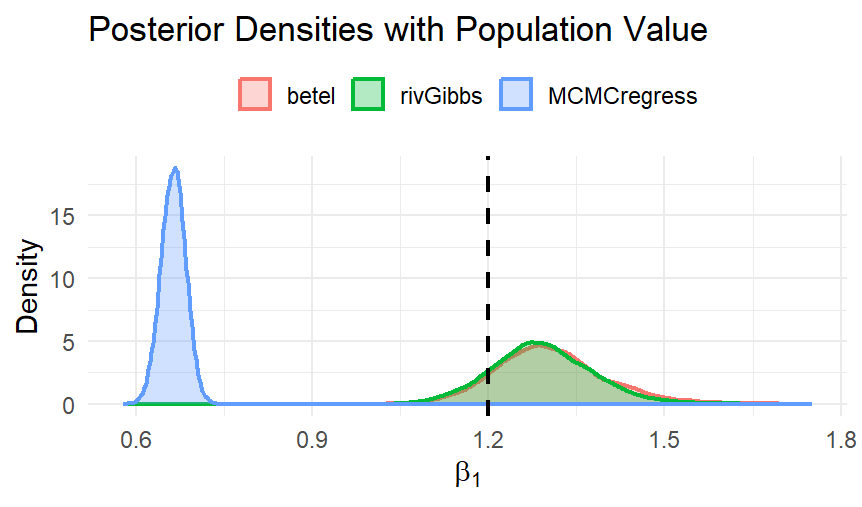
\includegraphics[width=340pt, height=200pt]{Chapters/chapter12/figures/FigME.png}
	\caption[List of figure caption goes here]{Posterior distribution slope parameter given measurement error: betel, ivGibbs and MCMCregress}\label{fig12_Measurement}
\end{figure} 
 
\textbf{Example: Omission of relevant correlated regressor}

Consider the true model
\[
Y_i = \beta_0 + \beta_1 X_i + \gamma W_i + \mu_i,
\qquad \mathbb{E}[\mu_i \mid X_i, W_i] = 0.
\]
Suppose that the relevant regressor $W_i$ is omitted from the specification, with $\gamma \neq 0$ and \(\operatorname{Cov}(X_i, W_i) \neq 0\).

Thus, if we regress $Y_i$ only on $X_i$, the composite error is
\[
\epsilon_i = \gamma W_i + \mu_i.
\]

Therefore,
\[
\mathbb{E}[\epsilon_i \mid X_i] 
= \gamma \, \mathbb{E}[W_i \mid X_i] + \mathbb{E}[\mu_i \mid X_i]
= \gamma \, \mathbb{E}[W_i \mid X_i] \neq 0,
\]
since $\mathbb{E}[W_i \mid X_i]$ is nonconstant whenever $X_i$ and $W_i$ are correlated, that is, the expected value of $W_i$ is a function of $X_i$.

Consequently,
\[
\mathbb{E}[\epsilon_i X_i] 
= \gamma \, \mathbb{E}[W_i X_i] + \mathbb{E}[\mu_i X_i].
\]
Because $\mathbb{E}[\mu_i X_i]=0$, we obtain
\[
\mathbb{E}[\epsilon_i X_i] = \gamma (\operatorname{Cov}(W_i,X_i) 
+ \mathbb{E}[W_i] \, \mathbb{E}[X_i])\neq 0.
\]

In this situation, we can use an instrument that is relevant ($\mathbb{E}[Z_i X_i] \neq 0$) and exogenous ($\mathbb{E}[Z_i \mid \mu_i] = \mathbb{E}[Z_i \mid W_i] = 0$) to address the endogeneity problem, and identify the causal effect.\footnote{Another potential solution for the omission of relevant variables is the use of \textit{proxy variables}; see \cite{wooldridge2010econometric} for details.} Therefore,
\[
\mathbb{E}\left[\begin{bmatrix}
	1\\
	Z_i
\end{bmatrix}(Y_i-\beta_0-\beta_1X_i)\right]=\mathbf{0}.
\] 

Figure~\ref{fig:DAG_OVB_IV} illustrates the case of an omitted relevant regressor that is correlated with $X_i$, and how an instrument can be used to identify the causal effect. The instrument resolves the endogeneity problem by exploiting variation in $X_i$ that is driven by $Z_i$, which is orthogonal to the problematic error term. In other words, it replaces ``bad'' correlation with ``clean'' variation.
 
\begin{figure}[h]
	\centering
	\begin{tikzpicture}[->,>=Stealth,shorten >=1pt,node distance=2.5cm,
		thick,main node/.style={circle,draw,minimum size=7mm}]
		% Nodes
		\node[main node]            (z)    {$Z$};
		\node[main node]            (x) [right=2.6cm of z] {$X$};
		\node[main node]            (y) [right=2.6cm of x] {$Y$};
		\node[main node, dashed]    (w) [above=1.8cm of x] {$W$};
		\node[main node, dashed]    (u) [above=1.8cm of y] {$\mu$};
		
		% Edges
		\path (x) edge (y)                    % causal effect of interest
		(w) edge (x)                    % omitted variable shifts X
		(w) edge (y)                    % omitted variable shifts Y (relevance)
		(z) edge (x)                    % instrument relevance
		(u) edge (y);                   % structural error
		
		% Optional curved arrow to highlight X-W correlation path
		% \draw[bend left=18] (z) to (x);
		
	\end{tikzpicture}
	\caption{DAG with omitted relevant regressor $W$ (dashed, unobserved) that is correlated with $X$ and affects $Y$, inducing endogeneity of $X$ in a regression of $Y$ on $X$. A valid instrument $Z$ affects $X$ (relevance) but has no direct path to $Y$ and is independent of $W$ and $u$ (exclusion/independence), enabling identification of the causal effect $X \to Y$.}
	\label{fig:DAG_OVB_IV}
\end{figure}

We ask in Exercise~10 to perform a simulation exercise to assess the ability of BETEL to identify the causal effect when an instrument is used to address the omission of relevant regressors.\\

\textbf{Example: Simultaneous causality}

This example is based on \cite{imbens2014ivperspective}, where Professor Imbens illustrates the problem of analyzing the causal effect on traded quantity of a tax of $100 \times r\%$ in a market. He defines the average causal effect on the logarithm of traded quantity as
\[
\tau = \mathbb{E}[q_i(r) - q_i(0)],
\]
where $q_i(r) = \log Q_i(r)$ and $Q_i(r)$ denotes the potential traded quantity if the tax were $r$\%.

This situation is more challenging than in the standard treatment effects literature, because we do not observe any unit facing the tax. Instead, we only observe all units facing no tax, that is, $Q_i^{\text{Obs}} = Q_i(0)$. This setting requires the use of a \textit{structural model} to define the counterfactual scenarios of the potential outcomes.

The starting point for inference on the treatment effect of this new tax is the price determination mechanism, that is, the assignment mechanism in the potential outcome framework. We specify a \textit{structural demand function} that defines the potential demand given the price (treatment) and other exogenous variables:
\[
q_i^d(p) = \beta_1 + \beta_2 p + \beta_3 y_i + \beta_4 pc_i + \beta_5 ps_i + u_{i1},
\]
where $q^d$ is demand, and $p$, $y$, $pc$, and $ps$ are the logarithms of price, income, the price of a complementary good, and the price of a substitute good, respectively. All coefficients are interpreted as demand elasticities. The term $u_{i1}$ represents unobserved demand factors such that $\mathbb{E}[u_{i1}]=0$. Therefore,
\[
\mathbb{E}[q_i^d(p)\mid p, y_i, pc_i, ps_i] = \beta_1 + \beta_2 p + \beta_3 y_i + \beta_4 pc_i + \beta_5 ps_i.
\]

This expectation does not represent the conditional expectation of the observed quantity in markets where the observed price equals $p$. Rather, it is the expectation of potential demand functions given $p$ and other exogenous controls, irrespective of the realized market price.

Similarly, the assignment mechanism requires specifying the \textit{structural supply function}:
\[
q_i^s(p) = \alpha_1 + \alpha_2 p + \alpha_3 er_i + u_{i2},
\]
which represents the quantity that sellers are willing to supply given the price and the (exogenous) exchange rate $er_i$. The unobserved supply factors satisfy $\mathbb{E}[u_{i2}]=0$, so that
\[
\mathbb{E}[q_i^s(p)\mid p, er_i] = \alpha_1 + \alpha_2 p + \alpha_3 er_i.
\]

This expectation represents the average of all potential supply functions given the price and exogenous controls, again irrespective of the realized market price.

Thus, the assignment mechanism is given by the market equilibrium where the observed price is such that the observed quantity is equal to the demand and supply potential outcomes at the observed price,
\[
q_i^{Obs}=q_i^d(p_i^{Obs})=q_i^s(p_i^{Obs}).
\] 
Using this market equilibrium condition, we get
\begin{align*}
	p_i^{Obs}=\pi_1+\pi_2 er_i + \pi_3 y_i + \pi_4 pc_i + \pi_5 ps_i + v_{i1},
\end{align*}
where $\pi_1=\frac{\alpha_1-\beta_1}{\beta_2-\alpha_2}$, $\pi_2=\frac{\alpha_3}{\beta_2-\alpha_2}$, $\pi_3=\frac{-\beta_3}{\beta_2-\alpha_2}$, $\pi_4=\frac{-\beta_4}{\beta_2-\alpha_2}$, $\pi_5=\frac{-\beta_5}{\beta_2-\alpha_2}$, and $v_{i1}=\frac{u_{i2}-u_{i1}}{\beta_2-\alpha_2}$ given $\beta_2\neq\alpha_2$, that is, the equations should be independent. This condition is given by economic theory due to $\beta_2<0$ and $\alpha_2>0$, the effect of price on demand and supply should be negative and positive, respectively.

The equation of price into the demand equation gives
\begin{align*}
	q_i^{Obs}=\tau_1+\tau_2 er_i + \tau_3 y_i + \tau_4 pc_i + \tau_5 ps_i + v_{i2},
\end{align*}

where $\tau_1=\beta_1+\beta_2\pi_1$, $\tau_2=\beta_2\pi_2$, $\tau_3=\beta_2\pi_3+\beta_3$, $\tau_4=\beta_2\pi_4+\beta_4$, $\tau_5=\beta_2\pi_5+\beta_5$, and $v_{i2}=\beta_2v_{i1}+u_{i1}$.

The expressions for $p_i^{Obs}$ and $q_i^{Obs}$ are called the \textit{reduced-form} representations. In Section \ref{sec71}, we presented the order condition, which is necessary, and the rank condition, which is both necessary and sufficient, to identify the structural parameters from the reduced-form parameters. A key point to note is that only the prior distribution of the reduced-form parameters is updated by the sample information, while the updating of the structural parameters occurs solely through the reduced-form parameters, that is,
\[
\pi(\boldsymbol{\beta},\boldsymbol{\alpha}\mid \boldsymbol{\gamma},\boldsymbol{\pi},\mathbf{W}_{1:N})
\;\propto\;
\pi(\boldsymbol{\beta},\boldsymbol{\alpha}\mid \boldsymbol{\gamma},\boldsymbol{\pi}).
\]
See Section~9.3 in \cite{zellner1996introduction} for details about identification in Bayesian inference. This implies that in \textit{under-identified} models, the posterior distribution of the structural parameters is not concentrated at a single point, but rather remains spread out (e.g., uniformly) over a range of values.\footnote{This identification issue is not peculiar to simultaneous equation models, it arises in other econometric/statistical models \cite{zellner1996introduction}. See for instance the example of the effects of vitamin A, Figures \ref{fig12_CACE} and \ref{fig12_LATE}.}

To analyze the causal effects of the new tax, we can find the new equilibrium,
\[
q_i^d(P_i(r)\times (1+r))=q_i^s(P_i(r)),
\] 
where $P_i(r)$ is the price level ($p_i(r)=\log P_i(r)$) that sellers get, and $(P_i(r)\times (1+r)$ is the price that buyers pay.

Let's define the (log) price that buyers pay $p_b = p + \log(1+r)$ while sellers receive $p$. The demand function becomes
\[
q_i^d\big(p + \log(1+r)\big) = \beta_1 + \beta_2\left(p + \log(1+r)\right) + \beta_3 y_i + \beta_4 pc_i + \beta_5 ps_i + u_{i1},
\]
and the supply function remains
\[
q_i^s(p) = \alpha_1 + \alpha_2 p + \alpha_3 er_i + u_{i2}.
\]

Thus, the equilibrium price is given by
\[
p_i^*(r) = \frac{(\beta_1 - \alpha_1) + \beta_3 y_i + \beta_4 pc_i + \beta_5 ps_i - \alpha_3 er_i + (u_{i1} - u_{i2}) + \beta_2 \log(1+r)}{\alpha_2 - \beta_2}.
\]

The equilibrium quantity is
\[
q_i^*(r) = \beta_1 + \beta_2\left(p_i^*(r) + \log(1+r)\right) + \beta_3 y_i + \beta_4 pc_i + \beta_5 ps_i + u_{i1}.
\]
Thus, the expected equilibrium price and quantity are
\[
\mathbb{E}[p_i^*(r)\mid y_i, pc_i, ps_i, er_i]
=
\frac{(\beta_1 - \alpha_1) + \beta_3 y_i + \beta_4 pc_i + \beta_5 ps_i - \alpha_3 er_i + \beta_2 \log(1+r)}{\alpha_2 - \beta_2},
\]
\[
\mathbb{E}[q_i^*(r)\mid y_i, pc_i, ps_i, er_i]
=
\alpha_1 + \alpha_2 \,\mathbb{E}[p_i^*(r)\mid \cdot] + \alpha_3 er_i.
\]
We can see that given $\beta_2 < 0 < \alpha_2$, we have:
\[
\frac{d p^*(r)}{dr} = \frac{\beta_2}{(\alpha_2 - \beta_2)(1+r)} < 0, \quad
\frac{d p_b^*(r)}{dr} = \frac{\alpha_2}{(\alpha_2 - \beta_2)(1+r)} > 0, \quad
\frac{d q^*(r)}{dr} = \alpha_2 \cdot \frac{d p^*(r)}{dr} < 0.
\]
Thus, the price received by sellers decreases with the tax, the price paid by buyers increases, and the equilibrium quantity falls.
  
Thus, the average causal effect on the logarithm of traded quantity as
\[
\tau = \mathbb{E}[q_i(r) - q_i(0)]= \frac{\alpha_2 \, \beta_2}{\alpha_2 - \beta_2}\,\log(1+r).
\]

Note that the treatment effect depends on the price elasticities of supply and demand. Therefore, we need to identify the demand and supply functions using instruments, since the observed quantities and prices cannot be used directly due to the issue of simultaneous causality. In particular, given the assumption of exogeneity of the other control variables, the only part of $p_i^{Obs}$ that can correlate with $u_{i1}$ or $u_{i2}$ is the error component
\[
\frac{u_{i2}-u_{i1}}{\beta_2-\alpha_2}.
\]

Hence
\[
\mathbb{E}[u_{i1}p_i^{Obs}]
=\frac{1}{\beta_2-\alpha_2}\,\mathbb{E}\!\big[u_{i1}(u_{i2}-u_{i1})\big]
=\frac{\operatorname{Cov}(u_{i1},u_{i2})-\operatorname{Var}(u_{i1})}{\beta_2-\alpha_2}\neq 0,
\]
and
\[
\mathbb{E}[u_{i2}p_i^{Obs}]
=\frac{1}{\beta_2-\alpha_2}\,\mathbb{E}\!\big[u_{i2}(u_{i2}-u_{i1})\big]
=\frac{\operatorname{Var}(u_{i2})-\operatorname{Cov}(u_{i1},u_{i2})}{\beta_2-\alpha_2}\neq 0,
\]

Due to the usual slopes $\beta_2<0<\alpha_2$ so that $\alpha_2-\beta_2>0$.

We can use supply shifters to identify the demand, and demand shifters to identify the supply. In this setting, the exchange rate serves as an instrument to identify the demand, while income together with the prices of complementary and substitute goods serve as instruments to identify the supply. Thus, we can use the moment conditions,
\[
\mathbb{E}\left[\begin{bmatrix}
	1\\
	y_i\\
	pc_i\\
	ps_i\\
	er_i
\end{bmatrix}(q_i^{Obs}-\beta_1-\beta_2p_i^{Obs}-\beta_3y_i-\beta_4pc_i-\beta_5ps_i)\right]=\mathbf{0},
\] 
and 
\[
\mathbb{E}\left[\begin{bmatrix}
	1\\
	y_i\\
	pc_i\\
	ps_i\\
	er_i
\end{bmatrix}(q_i^{Obs}-\alpha_1-\alpha_2p_i^{Obs}-\alpha_3er_i)\right]=\mathbf{0}
\]
to identify the demand and supply functions. Note that the demand equation is \textit{exactly identified}, whereas the supply equation is \textit{over identified}. See Section \ref{sec71} for details about identification of linear systems of equations.

We perform a simulation exercise to analyze the hypothetical causal effects of a new tax rate of 10\% simulating the demand and supply equations using the following structural parameters $\bm{\beta} = \left[ 5 \ -0.5 \ 0.8 \ -0.4 \ 0.7 \right]^{\top}$, $\bm{\alpha} = \left[ -2 \ 0.5 \ -0.4 \right]^{\top}$, $u_1 \sim N(0, 0.5^2)$, and $u_2 \sim N(0, 0.5^2)$ assuming a sample size equal to 5,000. Additionally, assume that $y \sim N(10, 1)$, $pc \sim N(5, 1)$, $ps \sim N(5, 1)$, and $er \sim N(15, 1)$. 

The population causal effect of the tax on quantity is
\[
\tau=\frac{(-0.5)\times 0.5}{0.5-(-0.5)}\log(1+0.1)\approx -0.0238,
\]
which implies that a \(10\%\) tax reduces traded quantity by approximately \(2.4\%\).

In Exercise~11, you are asked to program a BETEL algorithm from scratch to perform inference in this example. Figure~\ref{fig12_SimCausality} displays the posterior distribution of the causal effect. The 95\% credible interval contains the population value, and the posterior mean lies close to it.

\begin{figure}[h!]
	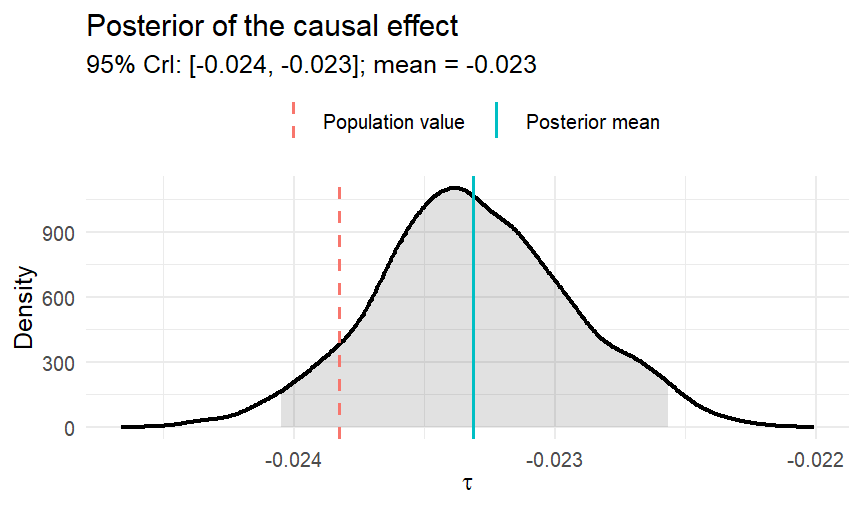
\includegraphics[width=340pt, height=200pt]{Chapters/chapter12/figures/fig12_SimCausality.png}
	\caption[List of figure caption goes here]{Posterior distribution of the causal effect of a tax: BETEL}\label{fig12_SimCausality}
\end{figure} 
  
\cite{chib2018moment} propose a unified framework based on marginal likelihoods and Bayes factors for comparing different moment-restricted models and for discarding misspecified restrictions. They demonstrate the model selection consistency of the marginal likelihood, showing that it favors the specification with the fewest parameters and the largest number of valid moment restrictions. When models are misspecified, the marginal likelihood procedure selects the model that is closest to the (unknown) true data-generating process in terms of Kullback–Leibler divergence. See \cite{lazar2021review, liu2023review} for comprehensive reviews of recent advances in empirical likelihood and exponentially tilted empirical likelihood methods, including their Bayesian variants.

\section{General Bayes posteriors}\label{sec12_10}

It is well known that, under model misspecification, that is, when the assumed likelihood function does not coincide with the true data-generating likelihood, the posterior concentrates its mass near those points in the support of the prior that minimize the Kullback--Leibler divergence with respect to the true model \cite{Kleijn2006}. However, this updating process may yield credible sets that fail to achieve the desired coverage, Bayes factors that can be misleading, and predictions that may remain approximately valid but require careful checking. In addition, the misspecified posterior distribution may exhibit suboptimal risk performance. In this setting, a modified posterior directly linked to the risk function of interest, known as the \textit{Gibbs posterior}, can still perform very well \cite{Jiang2008},
\begin{equation}\label{eq:GibbsPost}
	\hat{\pi}(\boldsymbol{\theta}\mid\mathbf{y})
	=\frac{\exp\left\{-Nw\,R_N(\boldsymbol{\theta},\mathbf{y})\right\}\pi(\boldsymbol{\theta})}
	{\int_{\boldsymbol{\Theta}}\exp\left\{-Nw\,R_N(\boldsymbol{\theta},\mathbf{y})\right\}\pi(\boldsymbol{\theta})\,d\boldsymbol{\theta}},
\end{equation}
where $w>0$ is the \textit{learning rate} (or the inverse temperature in simulated annealing), which balances the information in the data with that in the prior, $N$ is the sample size, and
\[
R_N(\boldsymbol{\theta},\mathbf{y})=\frac{1}{N}\sum_{i=1}^N l(\boldsymbol{\theta},\mathbf{y}_i)
\]
is the empirical risk associated with the loss function $l(\boldsymbol{\theta},\mathbf{y}_i)$.

Note that Equation~\ref{eq:GibbsPost} reduces to the ordinary Bayesian posterior when the loss is chosen as the negative log-likelihood, $l(\boldsymbol{\theta},y_i)=-\log p(y_i\mid\boldsymbol{\theta})$, under i.i.d.\ sampling and with $w=1$. In this case, we are asserting knowledge of the data-generating process $p(y_i\mid \boldsymbol{\theta})$. More generally, however, $R_N(\boldsymbol{\theta},\mathbf{y})$ can be based on any loss function that satisfies the required conditions for coherent belief updating: non-negativity, existence of a well-defined expectation, identifiability, and additivity across observations. Importantly, correctness of the parametric model is not required, since
\[
\frac{1}{N}\sum_{i=1}^N l(\boldsymbol{\theta},\mathbf{y}_i)\;\stackrel{p}{\longrightarrow}\;\int_{\mathcal{Y}} l(\boldsymbol{\theta},\mathbf{y})\,p(\mathbf{y}\mid \boldsymbol{\theta})\,d\mathbf{y},
\]
by the law of large numbers as $N\to\infty$.

Thus, the Gibbs posterior provides inference on the parameter values that minimize the chosen risk function, with minimal modeling assumptions. In contrast, the standard Bayesian posterior allows inference on essentially any feature of the data-generating distribution, but at the cost of strong model assumptions \cite{Syring2019}.

\cite{bissiri2016general} show that Equation~\ref{eq:GibbsPost} is a valid, coherent mechanism to update prior beliefs. In particular, there must exist a mapping $h$ such that
\[
\pi(\boldsymbol{\theta}\mid \mathbf{y}) = h\!\big(l(\boldsymbol{\theta},\mathbf{y}),\pi(\boldsymbol{\theta})\big),
\]
where $h$ satisfies the coherence property
\[
h\!\left[l(\boldsymbol{\theta},y_2),\,h\!\big(l(\boldsymbol{\theta},y_1),\pi(\boldsymbol{\theta})\big)\right]
= h\!\big(l(\boldsymbol{\theta},y_2)+l(\boldsymbol{\theta},y_1),\pi(\boldsymbol{\theta})\big).
\]
This ensures that the updated posterior $\pi(\boldsymbol{\theta}\mid y_1,y_2)$ is the same whether we update with $(y_1,y_2)$ jointly or sequentially.

Equation~\ref{eq:GibbsPost} is the solution of minimizing the loss function $L(\nu;\pi,\mathbf{y})$ on the space of probability measures on $\mathbf{\theta}-space$,
\[
\hat{\pi}=\arg\min_{\nu} L(\nu;\pi,\mathbf{y}),
\]
such that $\hat{\pi}$ is the representation of beliefs about $\boldsymbol{\theta}$ given prior beliefs ($\pi$) and data ($\mathbf{y}$). Given that the prior beliefs and the data are two independent pieces of information, it makes sense that the loss function is additive in these two arguments, 
\[
L(\nu;\pi,\mathbf{y})=h_1(\nu,\mathbf{y})+w^{-1}h_2(\nu,\pi),
\] 
where $h_1(\cdot)$ and $h_2(\cdot)$ are loss functions in their arguments.
The coherence requirement implies that
\[
h_2(\nu,\pi)=d_{KL}(\nu,\pi)=\int \log\frac{\nu(d\boldsymbol{\theta})}{\pi(d\boldsymbol{\theta})} \nu(d\boldsymbol{\theta}),
\]
that is, $h_2(\nu,\pi)$ must be the Kullback-Leibler divergence \cite{bissiri2016general}.

On the other hand, 
\[
h_1(\nu,\mathbf{y})=\int l(\boldsymbol{\theta},\mathbf{y})\nu(d\boldsymbol{\theta})
\]  
is the expected loss of the action with respect to the data.

Therefore, the minimizer of

\[
L(\nu;\pi,\mathbf{y})=\int l(\boldsymbol{\theta},\mathbf{y})\nu(d\boldsymbol{\theta})+d_{KL}(\nu,\pi),
\] 
is given by Equation~\ref{eq:GibbsPost} \cite{Zhang2006KLentropy,Jiang2008,bissiri2016general}.

A very important parameter in the Gibbs posterior \cite{Jiang2008}, or \textit{general Bayes posterior} \cite{bissiri2016general}, is the learning rate, as it determines the asymptotic sampling properties of $\hat{\pi}(\boldsymbol{\theta}\mid\mathbf{y})$ used to perform inference on $\boldsymbol{\theta}$. For instance, \cite{bissiri2016general} propose different strategies to set this parameter, and \cite{Syring2019} propose a Monte Carlo algorithm that selects the learning rate so that the resulting credible region attains the nominal Frequentist coverage probability.

\cite{chernozhukov2003mcmc} introduce the \emph{Laplace-type estimator} (LTE), which can be interpreted as a special case of the \emph{general Bayes} update of \cite{bissiri2016general}, taking as loss a scaled sample criterion based on the moment conditions (e.g., the GMM quadratic form).

In particular, given the moment conditions
\[
\mathbb{E}\!\big[\mathbf{g}_i(\mathbf{w}_i,\boldsymbol{\theta})\big]=\mathbf{0}_{d} 
\quad \text{if and only if } \boldsymbol{\theta}=\boldsymbol{\theta}_0,
\]
where the expectation is taken with respect to the population distribution, 
$\mathbf{w}_{1:N}:=[\mathbf{w}_1 \ \mathbf{w}_2 \ \dots \ \mathbf{w}_N]$ is a random sample from $\mathbf{W}\subset \mathbb{R}^{d_w}$, 
$\mathbf{g}:\mathbb{R}^{d_w}\times\boldsymbol{\Theta}\to\mathbb{R}^{d}$ is a vector of known functions, and 
$\boldsymbol{\theta}=[\theta_{1}\ \theta_{2}\ \dots\ \theta_{p}]^{\top}\in\boldsymbol{\Theta}\subset\mathbb{R}^{p}$ with $d\geq p$, the risk function can be defined as
\[
R_N(\boldsymbol{\theta},\mathbf{w})=\tfrac{1}{2}\left(\underbrace{\frac{1}{N}\sum_{i=1}^N \mathbf{g}_i(\mathbf{w}_i,\boldsymbol{\theta})}_{\mathbf{g}_N(\boldsymbol{\theta})}\right)^{\top}\mathbf{W}_N\left(\underbrace{\frac{1}{N}\sum_{i=1}^N\mathbf{g}_i(\mathbf{w}_i,\boldsymbol{\theta})}_{\mathbf{g}_N(\boldsymbol{\theta})}\right),
\]
where $\mathbf{W}_N$ is a positive semi-definite weighting matrix such that
\[
\mathbf{W}_N \;\to\; 
\Bigg(\text{Var}\left[\sqrt{N}\left(\tfrac{1}{N}\sum_{i=1}^N \mathbf{g}_i(\mathbf{w}_i,\boldsymbol{\theta}_0)\right)\right]\Bigg)^{-1}
\quad \text{as } N\rightarrow \infty.
\]  

Then, the \textit{quasi-posterior} in \cite{chernozhukov2003mcmc} is similar to Equation~\ref{eq:GibbsPost} with $w=1$.

Algorithm \ref{Alg:GibbsPosteior} shows the Metropolis-Hastings to perform inference using the general Bayes posterior.

\begin{algorithm}[h!]
	\caption{General Bayes posterior: Metropolis-Hastings algorithm}\label{Alg:GibbsPosteior}
	\begin{algorithmic}[1]
		\State Set $\bm{\theta}^{(0)}$ in the support of $\hat{\pi}(\bm{\theta}\mid \bm{y})$  		 			
		\For{\texttt{$s=1,\dots,S$}}
		\State Draw $\bm{\theta}^{c}$ from $q(\bm{\theta}^{c}\mid \bm{\theta}^{(s-1)})$
		\State Calculate $\alpha(\bm{\theta}^{(s-1)}, \bm{\theta}^{c}) = 
		\min\left\{\frac{q(\bm{\theta}^{(s-1)} \mid  \bm{\theta}^{c}) \exp\left\{-Nw\,R_N(\boldsymbol{\theta}^c,\mathbf{y})\right\}\pi(\boldsymbol{\theta}^c)}{q(\bm{\theta}^{c} \mid  \bm{\theta}^{(s-1)}) \exp\left\{-Nw\,R_N(\boldsymbol{\theta}^{(s-1)},\mathbf{y})\right\}\pi(\boldsymbol{\theta}^{(s-1)})}, 1\right\}$
		\State Draw $U$ from $U(0,1)$
		\State $\bm{\theta}^{(s)}=\begin{Bmatrix}
			\bm{\theta}^{c} & \text{if } U\leq \alpha(\bm{\theta}^{(s-1)}, \bm{\theta}^{c})\\
			\bm{\theta}^{(s-1)} & \text{otherwise}\\
		\end{Bmatrix}$
		\EndFor 
	\end{algorithmic} 
\end{algorithm}


Under suitable regularity conditions, \cite{chernozhukov2003mcmc} show that the LTE posterior mean is first-order equivalent to the efficient GMM estimator and that posterior quantiles yield confidence sets with asymptotically correct Frequentist coverage. Relatedly, \cite{Muller2013SandwichBayes} demonstrates that, under model misspecification, replacing the original likelihood with a curvature-adjusted (``sandwich") log-likelihood can improve Frequentist risk, that is, lower the average loss over repeated samples when making inference on the parameters. Moreover, \cite{ChenChristensenTamer2018} develop confidence sets based on quasi-posteriors that achieve exact asymptotic Frequentist coverage for identified sets of parameters in complex nonlinear structural models, regardless of whether the parameters are point identified. Finally, \cite{andrews2022weakgmm} study decision rules for weak GMM and provide support for quasi-Bayesian procedures built from the GMM quadratic form, in line with the spirit of the LTE in settings with weak identification.\\

\textbf{Example: Instrumental variable quantile regression (IVQR)}

\cite{Chernozhukov2005} propose an instrumental variable model of quantile treatment effects to characterize the heterogeneous impact of treatments across different points of the outcome distribution. Their model requires conditions that restrict the evolution of ranks across treatment states. Using these conditions, they address the endogeneity problem and recover quantile treatment effects using instrumental variables for the entire population, not only for compliers.  

Assume a binary treatment variable $D_i\in\{0,1\}$, with potential outcomes $\{Y_i(0),Y_i(1)\}$. The estimand of interest is the quantile treatment effect, which summarizes the differences in the quantiles of potential outcomes across treatment states,
\[
q(D_i=1,\mathbf{X}_i=\mathbf{x}_i,\tau)-q(D=0,\mathbf{X}_i=\mathbf{x}_i,\tau),
\] 
where $q(D_i=d,\mathbf{X}_i=\mathbf{x}_i,\tau)$ denotes the $\tau$-th quantile treatment response function.  

The potential outcomes are related to the quantile treatment response via
\[
Y_i(d)=q(D_i=d_i,\mathbf{X}_i=\mathbf{x}_i,U(d_i)),
\]
where $U(d_i)\sim U(0,1)$ is the \textit{rank variable}. This variable captures unobserved heterogeneity that explains differences in outcomes given observed characteristics $\mathbf{x}_i$ and treatment $d_i$.  

For instance, consider a retirement savings model, where the potential outcome is net financial assets under different retirement plan statuses $d$, and $q(D=d,\mathbf{X}=\mathbf{x},\tau)$ is the net financial asset function describing how an individual with retirement status $d$ and ``financial ability'' $\tau$ is rewarded in the financial market. Because the function depends on $\tau$, treatment effects are heterogeneous.  

The identification conditions for the IVQR model are stated in \cite{Chernozhukov2005} as follows:

\textit{1. Potential outcomes:}  
\[
Y_i(d)=q(D_i=d_i,\mathbf{X}_i=\mathbf{x}_i,U(d_i)),
\]
where $q(D_i=d_i,\mathbf{X}_i=\mathbf{x}_i,\tau)$ is strictly increasing in $\tau$ and $U(d_i)\sim U(0,1)$.  

\textit{2. Independence:} Conditional on $\mathbf{X}_i=\mathbf{x}_i$, the rank variables $\{U(d_i)\}$ are independent of the instruments $\mathbf{Z}_i$.  

\textit{3. Selection:} The treatment assignment is given by $D_i=\delta(\mathbf{Z}_i,\mathbf{X}_i,\mathbf{V}_i)$ for some unknown function $\delta$ and unobserved heterogeneity $\mathbf{V}_i$.  

\textit{4. Rank invariance:} Conditional on $\mathbf{X}_i=\mathbf{x}_i,\mathbf{Z}_i=\mathbf{z}_i$,

- either $\{U(d_i)\}$ coincide ($U(d_i)=U$ for all $d$), or
  
- $\{U(d_i)\}$ are identically distributed conditional on $\mathbf{V}_i$.  

\textit{5. Observables:} The observed data consist of $Y_i=q(D_i,\mathbf{X}_i,U(D_i))$, $D_i$, $\mathbf{X}_i$, and $\mathbf{Z}_i$, $i=1,2,\dots,N$.  

The most important identification restriction is \textit{rank invariance}, which implies that individuals with higher unobserved rank remain higher-ranked regardless of treatment status. This condition accommodates more general selection mechanisms than the monotonicity assumption used in the LATE framework, while being less restrictive than full independence assumptions between instruments ($\mathbf{Z}$) and unobserved variables in the selection equation ($\mathbf{V}$) in other common models (see \cite{chernozhukov2004effects,Chernozhukov2005} for details).\footnote{\cite{Chernozhukov2005}'s proposal allows for both discrete and continuous $D$ and $\mathbf{Z}$.} 

The main testable implication of the identification restrictions is that
\[
P\!\left(Y_i \leq q(D_i,\mathbf{X}_i,\tau)\mid \mathbf{X}_i,\mathbf{Z}_i\right)
= P\!\left(Y_i < q(D_i,\mathbf{X}_i,\tau)\mid \mathbf{X}_i,\mathbf{Z}_i\right)
= \tau,
\]
for all $\tau$ almost surely, and $U(D_i)\sim U(0,1)$ conditional on $(\mathbf{X}_i,\mathbf{Z}_i)$.  

This conditional moment restriction implies the unconditional moment conditions that form the basis for estimation and inference in the IVQR model \cite{chernozhukov2003mcmc,chernozhukov2004effects},
\[
\mathbf{g}_N(\boldsymbol{\theta})=\frac{1}{N}\sum_{i=1}^N (\tau-\mathbbm{1}(Y_i\leq \alpha_{\tau}D_i+\mathbf{X}_i^{\top}\boldsymbol{\beta}_{\tau}))\begin{bmatrix}
\mathbf{X}_i\\
\mathbf{Z}_i
\end{bmatrix}.
\]
Thus, the empirical risk function is given by 
\[
R_N(\boldsymbol{\theta},\mathbf{w})=\tfrac{1}{2}\mathbf{g}_N(\boldsymbol{\theta})^{\top}\mathbf{W}_N\mathbf{g}_N(\boldsymbol{\theta}),
\]
where
\[
\mathbf{W}_N=\frac{1}{\tau(1-\tau)}\left(\frac{1}{N}\sum_{i=1}^N \mathbf{Z}_i\mathbf{Z}_i^{\top}\right)^{-1}.
\]

The following code implements Algorithm~\ref{Alg:GibbsPosteior} to perform inference on the quantile treatment effect of participation in the 401(k) retirement program on net financial assets, using eligibility as an instrument (see the 401(k) treatment effects example in Section~\ref{chap12_4} for details of the data).

\begin{tcolorbox}[enhanced,width=4.67in,center upper,
	fontupper=\large\bfseries,drop shadow southwest,sharp corners]
	\textit{R code. Quantile treatment effects: 401(k) participation on net financial assets}
	\begin{VF}
		\begin{lstlisting}[language=R]	
rm(list = ls()); set.seed(10101)
# Load data
df <- read.csv("https://raw.githubusercontent.com/BEsmarter-consultancy/BSTApp/refs/heads/master/DataApp/401k.csv",
sep = ",", header = TRUE, quote = "")
# Attach variables
attach(df)
y <- net_tfa/1000    # Outcome: net financial assets
x <- as.vector(p401) # Endogenous regressor: participation
w <- as.matrix(cbind(age, inc, fsize, educ, marr, twoearn, db, pira, hown))  # Exogenous regressors
z <- as.matrix(e401)  # Instrument: eligibility (NO intercept here)
library(quantreg)
tau <- 0.5 
QuanReg <- rq(y ~ p401 + age + inc + fsize + educ + marr + twoearn + db + pira + hown, tau = tau, data = df)
summary(QuanReg)
Reg <- MCMCpack::MCMCquantreg(y ~ x + w, data = df, tau = tau)
BayesExo <- summary(Reg)
LossFunct <- function(par, tau, y, z, x, w){
	n <- length(y)
	X <- cbind(1, x, w)
	Z <- cbind(1, z, w)
	Ind <- as.numeric(y <= X%*%par) 
	gn <- colMeans((tau - Ind) * Z)
	Wni <- lapply(1:n, function(i) {Z[i,] %*% t(Z[i,])}) 
	Wn <- 1 / (tau * (1 - tau)) * solve(Reduce("+", Wni)/n)
	Ln <- - 0.5 * n * t(gn) %*% Wn %*% gn
	return(Ln)
}
par0 <- colMeans(Reg)
LossFunct(par = par0, tau = tau, y = y, z = z, x = x, w = w)
# ----- MH using Ln -----
k <- length(par0); b0 <- rep(0, k); B0 <- 1000*diag(k)
S <- 10000; burnin <- 10000; thin <- 1; tot <- S + burnin
BETA <- matrix(NA, tot, k); accept <- logical(tot)
SIGMA <- diag(BayesExo[["statistics"]][,2]); tune <- 2.4 / sqrt(k)
BETA[1,] <- par0
LL <- LossFunct(par = BETA[1,], tau = tau, y = y, z = z, x = x, w = w)
pb <- txtProgressBar(min=0, max=tot, style=3)
for(s in 2:tot){
	cand <- BETA[s-1,] + MASS::mvrnorm(1, rep(0, k), tune*SIGMA)
	LLc  <- LossFunct(par = cand, tau = tau, y = y, z = z, x = x, w = w)
	priorRat <- mvtnorm::dmvnorm(cand, b0, B0, log=TRUE) -
	mvtnorm::dmvnorm(BETA[s-1,], b0, B0, log=TRUE)
	loga <- (LLc - LL) + priorRat
\end{lstlisting}
	\end{VF}
\end{tcolorbox} 

\begin{tcolorbox}[enhanced,width=4.67in,center upper,
	fontupper=\large\bfseries,drop shadow southwest,sharp corners]
	\textit{R code. Quantile treatment effects: 401(k) participation on net financial assets}
	\begin{VF}
		\begin{lstlisting}[language=R]	
	if (is.finite(loga) && log(runif(1)) <= loga) {
		BETA[s,] <- cand; LL <- LLc; accept[s] <- TRUE
	} else {
		BETA[s,] <- BETA[s-1,]; accept[s] <- FALSE
	}
	if (s <= burnin && s %% 100 == 0) {    
		acc <- mean(accept[(s-99):s])
		if (acc > 0.35) tune <- tune * 1.25
		if (acc < 0.15) tune <- tune / 1.25
	}
	setTxtProgressBar(pb, s)
}
close(pb)
cat("\nAcceptance rate:", mean(accept), "\n")
keep <- seq(burnin, tot, by = thin)
cat("\nAcceptance rate:", mean(accept[keep]), "\n")
post <- BETA[keep, , drop=FALSE]   # posterior draws in scaled space
colnames(post) <- c("Int", "p401", "age", "inc", "fsize", "educ", "marr", "twoearn", "db", "pira", "hown")
# Posterior summaries
post_mean <- colMeans(post)
post_ci   <- apply(post, 2, quantile, c(0.025, 0.975))
round(post_mean, 3); round(post_ci, 3)
		\end{lstlisting}
	\end{VF}
\end{tcolorbox} 

Setting $\tau = 0.5$ (the median), the quantile treatment effect is USD 6,719, with a 95\% credible interval of (USD 6,612, USD 6,806). For $\tau = 0.9$, the treatment effect is USD 19,318, with a 95\% credible interval of (USD 18,634, USD 20,085). Note that, in the instrumental variable example, the posterior mean of the LATE was USD 8,520, which is higher than the treatment effect at the median ($\tau = 0.5$). This suggests that the LATE overstates the causal effect of 401(k) participation due to the large impact at higher quantiles of the outcome distribution.

\section{Doubly robust Bayesian inferential framework (DRB)}\label{sec12_11}

\cite{breunig2025double} propose a doubly robust Bayesian (DRB) approach to perform inference on the average treatment effect (ATE) under unconfoundedness. They adjust the prior for the conditional mean outcome function using an estimator of the propensity score, the conditional probability of treatment assignment \cite{rosenbaum1983central}, and then re-center the posterior distribution of the treatment effect using the propensity score estimator together with a pilot estimator of the outcome regression. The authors show that under unconfoundedness and overlap, the corrected posterior converges in distribution to a normal law centered at a semiparametrically efficient estimator, and that the resulting credible intervals achieve asymptotically exact Frequentist coverage.

Let $Y_i\in\{0,1\}$ be the outcome and $D_i\in\{0,1\}$ the treatment,\footnote{\cite{breunig2025double} extend their framework to continuous, counting and multinomial outcomes.} thus
\[
Y_i = D_i\,Y_i(1) + (1-D_i)\,Y_i(0),
\]
where $Y_i(1)$ and $Y_i(0)$ are the potential outcomes.

Let $\mathbf{X}_i$ denote pre-treatment covariates with distribution $F_0$ and density $f_0$, and define the propensity score
\[
\pi_0(\mathbf{x}) := P(D_i=1\mid \mathbf{X}_i=\mathbf{x})
\]
and the conditional mean outcome (success probability)
\[
m_0(d,\mathbf{x}) := P(Y_i=1\mid D_i=d,\mathbf{X}_i=\mathbf{x}).
\]
For an i.i.d. sample $W_i=(Y_i,D_i,\mathbf{X}_i^{\top})^{\top}$, the joint density can be written as
\[
p_{f,\pi,m}(y,d,\mathbf{x})
= f(\mathbf{x})\,[\pi(\mathbf{x})]^d\,[1-\pi(\mathbf{x})]^{1-d}\,[m(d,\mathbf{x})]^y\,[1-m(d,\mathbf{x})]^{1-y}.
\]
The parameter of interest is the average treatment effect (ATE),
\[
\tau := \mathbb{E}_0\!\left[\,Y_i(1)-Y_i(0)\,\right],
\]
where $\mathbb{E}_0$ is the expectation with respect to the population distribution.

\cite{breunig2025double} impose support restrictions via link functions. For the outcome regression and propensity score use logits:
\[
m_\eta(d,\mathbf{x})=\frac{1}{1+\exp\{-\eta^m(d,\mathbf{x})\}},
\qquad
\pi_\eta(\mathbf{x})=\frac{1}{1+\exp\{-\eta^\pi(\mathbf{x})\}},
\]
so that
\[
\eta^m(d,\mathbf{x})=\log\!\left(\frac{m_\eta(d,\mathbf{x})}{1-m_\eta(d,\mathbf{x})}\right),
\qquad
\eta^\pi(\mathbf{x})=\log\!\left(\frac{\pi_\eta(\mathbf{x})}{1-\pi_\eta(\mathbf{x})}\right).
\]
For the covariate density, they use a log-density parametrization
\[
f_\eta(\mathbf{x})=\exp\{\eta^f(\mathbf{x})\},
\qquad
\eta^f(\mathbf{x})=\log f_\eta(\mathbf{x}).
\]
Given a prior on $(\eta^m,\eta^\pi,\eta^f)$, the induced ATE is
\[
\tau_\eta := \mathbb{E}_\eta\!\left[m_\eta(1,\mathbf{X})-m_\eta(0,\mathbf{X})\right].
\]

% EIF
The basis for inference on $\tau_\eta$ is the \textit{efficient influence function} (EIF):
\[
\tilde{\tau}_\eta(W)
= \big\{m_\eta(1,\mathbf{X})-m_\eta(0,\mathbf{X})\big\}
+ \gamma_\eta(D,\mathbf{X})\,\big\{Y-m_\eta(D,\mathbf{X})\big\}
- \tau_\eta,
\]
where the Riesz representer for the ATE functional is
\[
\gamma_\eta(D,\mathbf{X})
= \frac{D}{\pi_\eta(\mathbf{X})}
- \frac{1-D}{1-\pi_\eta(\mathbf{X})}.
\]

% Properties and DR
An influence function measures the first-order effect of an infinitesimal contamination of the underlying distribution on the estimand. The \emph{efficient} influence function attains the semiparametric efficiency bound (its variance is the minimal asymptotic variance in the model). At the truth $\eta_0$, the EIF is mean-zero: $\mathbb{E}_0[\tilde{\tau}_{\eta_0}(W)]=0$. Moreover, it is \emph{doubly robust}:
\[
\mathbb{E}_0\!\big[\tilde{\tau}_\eta(W)\big]=0
\quad\text{if either } m_\eta \text{ or } \pi_\eta \text{ is correctly specified.}
\]

To conduct Bayesian inference, \cite{breunig2025double} place independent priors on the outcome regression and the covariate distribution (equivalently, on $\eta^m$ and $\eta^f$). For the covariates they use a Dirichlet Process (DP) prior on $F$ (hence on $f$; see Section \ref{sec11_12}), which, under standard conditions, induces posterior draws that approximate the Bayesian bootstrap for sample supported functionals \cite{Lo1987BayesianBootstrap} (see Section \ref{sec610}). 

For the outcome regression they place a Gaussian Process (GP) prior on $\eta^m$ (see Section \ref{13_4}), with a correction term that incorporates a preliminary estimator of the Riesz representer. The propensity score is estimated in a separate first step and is used in the correction/recentering; thus, a prior for $\eta^\pi$ is not required for their procedure.

Algorithm~\ref{Alg:DRBayes} outlines the doubly robust Bayesian procedure of \cite{breunig2025double}. 
The pilot estimate of the Riesz representer, $\hat\gamma_\eta$, is obtained by plug–in, using a propensity score $\hat\pi(\mathbf{x})$ estimated via logistic Lasso.
 
The pilot estimate of the outcome regression, $\hat m_\eta(d,\mathbf{x})=\Pr(Y=1\mid D=d,\mathbf{X}=\mathbf{x})$, is taken as the posterior mean from a GP \emph{classification} model fit with a Laplace approximation.

Concretely, place a GP prior on the latent logit
$\eta^m(d,\mathbf{x})$ with a squared exponential kernel, and map to
success probabilities via the logistic link
$m(d,\mathbf{x})=\operatorname{logit}^{-1}\{\eta^m(d,\mathbf{x})\}$.
Because the Bernoulli likelihood makes the required integrals over
$\eta^m$ analytically intractable, the posterior is approximated using
Laplace’s method (Expectation Propagation is a common alternative).
See Sections 3.3–3.5 of \cite{rasmussen2006gaussian} for details.

The \emph{adjusted} GP prior specifies the latent logit as
\[
\eta^m(d,\mathbf{x}_i)
\;=\;
W^m(d,\mathbf{x}_i)\;+\;\lambda\,\widehat{\gamma}_\eta(d,\mathbf{x}_i),
\qquad
W^m \sim \mathrm{GP}\!\big(0, K\big),\ \ \lambda \sim N(0,\sigma_n^2),
\]
where $K$ is the base kernel. Following \cite{breunig2025double},
take
\[
\sigma_n \;=\; \frac{\log n}{\sqrt{n}\,\Gamma_n},
\qquad
\Gamma_n \;:=\; \frac{1}{n}\sum_{i=1}^n
\big|\widehat{\gamma}_\eta(d_i,\mathbf{x}_i)\big|.
\]
Since $W^m$ and $\lambda$ are Gaussian, this is equivalent to a GP with
an augmented kernel,
\[
\eta^m \sim \mathrm{GP}\!\big(0,\, K_c\big),
\quad
K_c\big((d,\mathbf{x}),(d',\mathbf{x}')\big)
= K\big((d,\mathbf{x}),(d',\mathbf{x}')\big)
+ \sigma_n^2\,\widehat{\gamma}_\eta(d,\mathbf{x})\,
\widehat{\gamma}_\eta(d',\mathbf{x}'),
\]
which, for the vector of latent logits evaluated at the training inputs,
corresponds to the covariance matrix
$\mathbf{K} + \sigma_n^2\,\widehat{\boldsymbol{\gamma}}\,
\widehat{\boldsymbol{\gamma}}^{\top}$. 

\begin{algorithm}[h!]
	\caption{Double Robust Bayesian Algorithm}\label{Alg:DRBayes}
	\begin{algorithmic}[1]
		\State Have initial estimates of $\hat{\gamma}_{\eta}$ based on logistic Lasso
		\State Trim the propensity score using standard values, for instance, 10\%, or the optimal trimming rule proposed by \cite{Crump2009Overlap}
		\State Estimate the Riesz representer using the estimate of the propensity score 
		\State Calculate the prior correction term $\sigma_n=\frac{\log(n)}{n^{1/2}\Gamma_n}$, $\Gamma_n=\frac{1}{n}\sum_{i=1}^n |\hat{\gamma}_{\eta}(d_i,\mathbf{x}_i)|$, $n$ is the effective sample size (after trimming)
		\State Calculate the prior adjustment $\sigma_n\times \hat{\gamma}_{\eta}$ 
		\State Calculate $\hat{m}(d,\mathbf{x})=\frac{1}{1+\exp\left\{-\eta^m(d,\mathbf{x})\right\}}$ as the posterior mean of a Gaussian Process (GP) based on $d$ and $\mathbf{x}$ (unadjusted mean)
		\State Set an initial GP prior for  the adjusted mean $m_{\eta}^c(d,\mathbf{x})=\frac{1}{1+\exp\left\{-\eta^m\right\}}$, where $\eta^m \sim \mathrm{GP}\!\big(0,\, K_c\big)$, $K_c\big((d,\mathbf{x}),(d',\mathbf{x}')\big)
		= K\big((d,\mathbf{x}),(d',\mathbf{x}')\big)
		+ \sigma_n^2\,\widehat{\gamma}_\eta(d,\mathbf{x})\,
		\widehat{\gamma}_\eta(d',\mathbf{x}')$ 		 			
		\For{\texttt{$s=1,\dots,S$}} 
		\State Generate the $s-th$ draw of the adjusted GP posterior, $m_{\eta}^{c,s}(d,\mathbf{x})$
		\State Draw Bayesian bootstrap weights $M^s_{ni}=\frac{e_i^s}{\sum_{j=1}^n e_j^s}$, $e_i^s\sim Exp(1)$, $i=1,2,\dots,n$
		\State Calculate the corrected posterior draw for the ATE $\tilde{\tau}_{\eta}^s=\tau_{\eta}^s-\hat{b}_{\eta}^s$, where $\tau_{\eta}^s=\sum_{i=1}^n M^s_{ni}(m_{\eta}^{c,s}(1,\mathbf{x}_i)-m_{\eta}^{c,s}(0,\mathbf{x}_i))$, and $\hat{b}_{\eta}^s=\frac{1}{n}\sum_{i=1}^n\tau[m_{\eta}^s(\mathbf{w}_i)-\hat{m}(\mathbf{w}_i)]$, $\tau[m]=m(1,\mathbf{x})-m(0,\mathbf{x})+\hat{\gamma}(d,\mathbf{x})(y-m(d,\mathbf{x}))$ 
		\EndFor 
	\end{algorithmic} 
\end{algorithm}      
 
Algorithm~\ref{Alg:DRBayes} produces posterior draws of the ATE. The $(1-\alpha)\%$ credible interval is given by the empirical quantiles at levels $\alpha/2$ and $1-\alpha/2$. 

It is worth noting that \cite{breunig2025double} do not perform sample splitting, whereas \cite{chernozhukov2018double} recommend it in the context of \textit{Double/Debiased Machine Learning for treatment and structural parameters}. While sample splitting (or cross-fitting) helps reduce overfitting, its role in \cite{chernozhukov2018double} is more fundamental: it ensures that the nuisance functions are estimated on data independent of the observations used for inference, which is critical for their theoretical guarantees of $\sqrt{n}$-consistency and valid asymptotic inference. Nevertheless, \cite{breunig2025double} report that they did not find evidence of overfitting in their setting and verified that their results are robust to the use of sample splitting.

Finally, observe that the doubly robust approach does not propagate the uncertainty due to the estimation of the propensity score, which is treated as a plug-in. This omission is justified because the efficient influence function (EIF) is \textit{Neyman orthogonal}: estimation error in the propensity score enters only at second order and is therefore asymptotically negligible for uncertainty quantification.\\

\textbf{Example: Doubly robust Bayesian inference}

Let us simulate the process 
\[
\eta^{\pi}_i = -0.3 + 0.8X_{i1} - 0.5X_{i2} + 0.7X_{i3}, 
\quad 
\eta^{m}_i = -0.2 + 0.6D_i + 0.5X_{i1} - 0.4X_{i2} + 0.3X_{i3},
\]
where $X_{1}\sim N(0,1)$, $X_{2}\sim \mathrm{Bernoulli}(0.5)$, and $X_{3}\sim U(-1,1)$, and the sample size is 2,000.
 
The population ATE from this simulation is approximately $0.138$. The posterior mean and 95\% credible interval of the ATE using the DRB are $0.155$ and $(0.107,\,0.206)$, respectively. 

The following code shows how to implement the DRB inferential framework in this setting.

\begin{tcolorbox}[enhanced,width=4.67in,center upper,
	fontupper=\large\bfseries,drop shadow southwest,sharp corners]
	\textit{R code. Doubly robust Bayesian inference: Simulation exercise}
	\begin{VF}
		\begin{lstlisting}[language=R]	
######### Doubly Robust Bayesian: Simulation #########
rm(list = ls()); set.seed(123); library(glmnet)
## simulate covariates
n  <- 2000
X1 <- rnorm(n)                 # continuous
X2 <- rbinom(n, 1, 0.5)        # binary
X3 <- runif(n, -1, 1)          # continuous
Z <- cbind(X1, X2, X3)
# True propensity and outcome
logit <- function(t) 1/(1+exp(-t))
true_pi  <- function(X){ logit(-0.3 + 0.8*X[,1] -0.5*X[,2] + 0.7*X[,3]) }
true_eta <- function(d,X){ -0.2 + 0.6*d + 0.5*X[,1] -0.4*X[,2] + 0.3*X[,3] }
true_p   <- function(d,X){ logit(true_eta(d,X)) }
ATE  <- mean(true_p(1,Z) - true_p(0,Z)) # Population ATE
# Data
pi <- true_pi(Z); D  <- rbinom(n,1,pi)
P  <- true_p(D,Z); Y  <- rbinom(n,1,P)
dat <- data.frame(Y, D, X1, X2 = factor(X2), X3)
######### Doubly Robust Bayesian: Implementation #########
p <- dim(Z)[2]; covars <- c("X1","X2","X3")
Z.df <- as.data.frame(Z) # covariates as a dataframe
# Propensity score model: lasso
cvfit <- cv.glmnet(Z, D, family = "binomial", alpha=1, nfolds = 10) # lasso,min
ps.coef <- coef(cvfit, s = "lambda.min")[0:p+1]
ps_hat <- predict(cvfit, newx = Z, s = "lambda.min",type = "response")
ps_hat <- pmin(pmax(ps_hat, 1e-6), 1 - 1e-6)
# Riesz representer
riesz_fun <- function(d, ps) d/ps - (1 - d)/(1 - ps)
# GP model
make_gp <- function(X_train, y_bin, use_correction = FALSE, gamma_scaled = NULL,
approx_method = gplite::approx_laplace(),
init_lscale = 0.3) {
	stopifnot(length(y_bin) == nrow(X_train))
	# Initializing the covariance function
	cf_se <- gplite::cf_sexp(vars = colnames(X_train), lscale = init_lscale, magn = 1, normalize = TRUE)
	cfs <- list(cf_se)
	if (use_correction) {
		stopifnot(!is.null(gamma_scaled))
		# Add linear kernel on the last column (gamma_scaled)
		cf_lin <- gplite::cf_lin(vars = "gamma", magn = 1, normalize = FALSE)
		cfs <- list(cf_se, cf_lin)
	}
	# Initializes a GP model
	gp <- gplite::gp_init(cfs = cfs, lik = gplite::lik_bernoulli(), approx = approx_method)
	# Optimizing hyperparameters
	gp <- gplite::gp_optim(gp, x = X_train, y = y_bin, maxiter = 1000, restarts = 3, tol = 1e-05)
	return(gp)
}
\end{lstlisting}
\end{VF}
\end{tcolorbox} 

\begin{tcolorbox}[enhanced,width=4.67in,center upper,
	fontupper=\large\bfseries,drop shadow southwest,sharp corners]
	\textit{R code. Doubly robust Bayesian inference: Simulation exercise}
	\begin{VF}
		\begin{lstlisting}[language=R]	
posterior_draws_prob <- function(gp, X_test, ndraws = 5000) {
	out <- gplite::gp_draw(gp, xnew = X_test, draws = ndraws, transform = TRUE, target = FALSE, jitter = 1e-6)
	return(t(out))
}
# Main function
run_trim <- function(t_trim = 0.10, N_post = 5000, h_r = 1/2, cor_size = 1) {
	# Trim by estimated PS
	keep <- which(ps_hat >= t_trim & ps_hat <= (1 - t_trim))
	n_eff <- length(keep)
	if (n_eff < 50) stop("Too few observations after trimming.")
	Yk  <- Y[keep]
	Dk  <- D[keep]
	Zk  <- Z[keep, , drop = FALSE]
	psk <- ps_hat[keep]
	# Riesz representer and sigma_n choice
	gamma_k <- riesz_fun(Dk, psk)
	sigma_n <- cor_size * (log(n_eff) / ( (n_eff)^(h_r) * mean(abs(gamma_k)) ))
	gamma_scaled <- sigma_n * gamma_k
	# Training inputs for GP: [Z, D] and, if corrected, an extra column 'gamma'
	X_train_nc <- data.frame(Zk)
	X_train_nc$D <- Dk
	colnames(X_train_nc) <- c(covars, "D")
	X_train_c <- X_train_nc
	X_train_c$gamma <- gamma_scaled
	# Test inputs: for each i, (Z_i, d=0) and (Z_i, d=1)
	X_t0 <- X_train_nc; X_t0$D <- 0
	X_t1 <- X_train_nc; X_t1$D <- 1
	X_t0c <- X_t0; X_t1c <- X_t1
	X_t0c$gamma <- sigma_n * riesz_fun(0, psk)   
	X_t1c$gamma <- sigma_n * riesz_fun(1, psk) 
	# GP WITHOUT prior correction #
	gp_nc <- make_gp(X_train = X_train_nc, y_bin = Yk, use_correction = FALSE)
	# joint draws for [m(Z,0); m(Z,1)]
	M_nc_0 <- posterior_draws_prob(gp_nc, X_t0, ndraws = N_post)  # N_post x n_eff
	M_nc_1 <- posterior_draws_prob(gp_nc, X_t1, ndraws = N_post)
	# observed arm probabilities
	M_nc_obs <- ifelse(matrix(Dk, nrow = N_post, ncol = n_eff, byrow = TRUE) == 1, M_nc_1, M_nc_0)
	# GP WITH prior correction #
	gp_c <- make_gp(X_train = X_train_c, y_bin = Yk, use_correction = TRUE, gamma_scaled = gamma_scaled)
	M_c_0 <- posterior_draws_prob(gp_c, X_t0c, ndraws = N_post)
	M_c_1 <- posterior_draws_prob(gp_c, X_t1c, ndraws = N_post)
	M_c_obs <- ifelse(matrix(Dk, nrow = N_post, ncol = n_eff, byrow = TRUE) == 1, M_c_1, M_c_0)
\end{lstlisting}
	\end{VF}
\end{tcolorbox} 

\begin{tcolorbox}[enhanced,width=4.67in,center upper,
	fontupper=\large\bfseries,drop shadow southwest,sharp corners]
	\textit{R code. Doubly robust Bayesian inference: Simulation exercise}
	\begin{VF}
		\begin{lstlisting}[language=R]	
	# Bayesian bootstrap weights #
	W <- matrix(rexp(N_post * n_eff, rate = 1), nrow = N_post)
	W <- W / rowSums(W)
	# ATEs
	# (1) Unadjusted Bayes
	Ate_nc_draws <- rowSums((M_nc_1 - M_nc_0) * W)
	# (2) Prior-adjusted Bayes
	Ate_c_draws  <- rowSums((M_c_1 - M_c_0) * W)
	# (3) DR Bayes (posterior recentering)
	# Pre-centering using UNcorrected GP posterior means
	mu_nc_diff <- colMeans(M_nc_1 - M_nc_0)                
	mu_nc_obs  <- colMeans(M_nc_obs)                       
	ATE_dr_pre <- mean(mu_nc_diff + gamma_k * (Yk - mu_nc_obs))
	# Recenter draws using corrected GP draws
	DR_rec_1 <- (matrix(gamma_k, nrow = N_post, ncol = n_eff, byrow = TRUE)) * (matrix(Yk, nrow = N_post, ncol = n_eff, byrow = TRUE) - M_c_obs)
	# The first component is \tau_{\eta}^s in Algorithm 1
	# The second component is \hat{m} a scalar. This has positive sign because
	# minus x minus, the bias is with minus, and then, this component enters with minus in the bias term
	# The third component is \gamma_k x (y-m(d,x)), m(d,x) is with prior correction
	# The fourth component is m(1,x)-m(0,x) also with correction in the prior
	Ate_drb_draws <- rowSums((M_c_1 - M_c_0) * W) + ATE_dr_pre - rowSums(DR_rec_1) / n_eff - rowSums(M_c_1 - M_c_0) / n_eff
	
	qfun <- function(x) {
		qs <- quantile(x, c(0.025, 0.975))
		c(mean   = mean(x), 	median = median(x), lo = qs[1],	hi = qs[2],	len = diff(qs)
		)
	}	
	vals <- list(
	Bayes      = qfun(Ate_nc_draws),
	`PA Bayes` = qfun(Ate_c_draws),
	`DR Bayes` = qfun(Ate_drb_draws)
	)
	out_df <- as.data.frame(do.call(rbind, vals), check.names = FALSE)
	list(t_trim = t_trim, results = out_df)
}
N_post <- 5000
h_r    <- 1/2
cor_size <- 1
trim <- 0.05
res_list <- run_trim(t_trim = trim, N_post = N_post, h_r = h_r, cor_size = cor_size)
print(res_list$results)
\end{lstlisting}
	\end{VF}
\end{tcolorbox} 

\begin{comment}
\section{Other approaches}\label{sec12_12}
There are other causal inference approaches that we do not cover in this chapter but are worth mentioning. In particular, 

Another interesting approach is the synthetic control method, which estimates a treatment effect by constructing a weighted combination of untreated units that best matches the treated unit's pre-treatment outcomes, and then comparing post-treatment differences. Identification relies on \textit{no interference between units}, \textit{parallel trends between the treated unit and its synthetic control in the absence of treatment}, and \textit{no anticipation of treatment} \cite{abadie2010synthetic}. Several proposals extend this framework to the Bayesian setting \cite{amjad2018robust,kim2020bayesian,pang2022bayesian}.

%%%%%%%%%%%%%%%%%%%%%%%%%%%%%%%%%%%%%%%%%%%%%%%%%%%%%%%%%%%%%%%%%%%%%%%%%%  

Remember the role of $\rho$, the correlation of the potential outcomes $Y(1)$ and $Y(0)$, where the likelihood does not have information about it!

In this framework, there is a model for the assignment mechanism $P(D_i\mid Y_i(1), Y_i(0), \mathbf{X}_i)$, like randomization or propensity score matching \cite{rosenbaum1983central}, supplemented by a model for the data $P(Y_i(1), Y_i(0)\mid \mathbf{X}_i)$. A causal inference is delivered by conditioning in what is observed to calculate the posterior distribution of the causal estimand given also the models for the assignment mechanisms and data. Therefore, there is a model to input the potential outcome missing value that allows to get the predictive distribution, and then, the posterior predictive distribution of the treatment effect ($Y_i(1)-Y_i(0)$) is calculated. We should take into account that the parameters of the models for predicting the missing potential outcomes are generally not causal effects. Due to using models for the data based on simulation, the Bayesian approach is by far the most direct and flexible of the modes of inference for causal effects. However, it relies on assumptions on the assignment mechanism and data.

Given pretreatment variables, it improves the predictive power of the potential outcome missing data

There, no compliance is explicitly treated as missing data. A nice advantage of the Bayesian approach is to relax the exclusion restriction \cite{rubin2004teaching}.

Propensity matching should be used to create ``assigned treatment" and ``assigned control" groups that are well balanced on all covariates. The covariate modeling should be applied to estimate the effects of ``received treatment" for the subgroup of true compliers \cite{rubin2004teaching}.

Simultaneous causality is conceptually challenging because causality is often associated with chronological order, cause preceding effect. In simultaneous systems, such as supply and demand, outcomes are jointly determined in equilibrium, so this temporal order is not explicit in the observed data. Nevertheless, the underlying structural equations still encode causal relationships, even though their effects are realized simultaneously.

In general, association does not imply causation, although causation does imply association. Two variables can be associated for several reasons: one may cause the other, they may share common causes, or they may share a common effect when the analysis is restricted to a specific level of that effect (or one of its descendants) \cite{hernan2020causal}. For this reason, causal graphs are valuable tools for explicitly representing the assumptions about the causal relationships under study and should be among the first steps in establishing an identification strategy.

Introduce maximum entropy using identification conditions to build likelihood functions.

Instrumental variables change the level of the treatment, without affecting the potential outcomes associated with these treatment levels \cite{imbens2014ivperspective}.

The gold standard in identification of causal effects is \textit{randomized controlled trial (RCT)}, where assignment to treatment is random, independent of the outcome and other potential exogenous determinants of the outcome. However, most of the time practitioners use \textit{observational data}, where the treatment status/level is \textit{endogenous} due to units actively defining the treatment that they receive \cite{imbens2014ivperspective}. Thus the assignment mechanism in RCTs are given by chance, whereas in observational studies by choice. This makes a subtantial methodological difference such that the latter implies looking a source of \textit{exogenous variation} that influences the \textit{treatment status/level}.

Two critical aspects in the identification of causal effects are: (i) the presence of a strong source of \textit{exogenous variation} that influences the \textit{endogenous regressors}, which are often the primary variables of interest to researchers, as they may directly affect the outcome or response variables and can be influenced by policy decisions, for example, identifying the causal effects of social programs on income or education, or evaluating strategic interventions in industry, such as estimating the price elasticity of demand for a specific product; and (ii) the effective \textit{control of other relevant exogenous covariates}, such as pre-treatment characteristics or external factors in a demand model.

In this context, the use of \textit{non-parametric models} (see Chapters~\ref{chap12} and~\ref{chap13}) is valuable due to their flexibility and weaker structural assumptions. Therefore, non-parametric and machine learning approaches serve as \textit{powerful tools} that can be combined with strong exogenous variation to robustly identify causal effects \cite{chernozhukov2018double,chernozhukov2024applied}.

Read this reference \cite{iacovone2023bayesian} before begin working in this chapter! Also read \cite{imbens1997bayesian}.

%\section{Bayesian model averaging}\label{sec12_10}
%We can use BMA as a sensible way to perform robustness analysis regarding model specification (regressors uncertainty) in performing inference of treatment effects.

%\section{Double-Debiased machine learning causal effects}\label{sec12_11a}
\end{comment}

\section{Summary}

In this chapter, we review some of the most common approaches to causal inference. We begin by outlining the identification restrictions underlying each method and then describe how these restrictions are incorporated into a Bayesian framework for inference. A natural point of departure is the use of Directed Acyclic Graphs (DAGs), which provide a graphical representation of the underlying structural or causal model. The next step is to identify an exogenous source of variation in the assignment rule, such as instruments or institutional arrangements, whose variability enables the identification of the causal effect of the treatment or relevant regressor on the outcome.

Given such sources of variation, one can use parametric, semiparametric, or nonparametric models to specify the conditional means of the potential outcomes given treatment assignment, thereby constructing counterfactual scenarios and enabling inference on causal estimands, such as the average treatment effect. Particular attention must be paid to the correct specification of the treatment assignment mechanism (propensity score) and the outcome regression, as both play a crucial role in credible causal inference. 

This highlights the growing importance of modern machine learning methods for estimating high-dimensional or complex nuisance functions (see Chapter \ref{chap13} and Section \ref{sec12_11}). At the same time, however, it is essential to address and correct for the biases that machine learning methods may introduce in order to obtain valid causal inference.

Finally, the Bayesian framework provides a coherent way to integrate these identification strategies with prior information and to obtain full posterior distributions of causal estimands, based on both the marginal distributions of the potential outcomes and their joint distribution, thereby offering a unified approach to causal inference.


%There are other causal inference approaches that we do not cover in this chapter. For instance, the synthetic control method, which estimates a treatment effect by constructing a weighted combination of untreated units that best matches the treated unit's pre-treatment outcomes, and then comparing post-treatment differences. Identification relies on \textit{no interference between units}, \textit{parallel trends between the treated unit and its synthetic control in the absence of treatment}, and \textit{no anticipation of treatment} \cite{abadie2010synthetic}. Several proposals extend this framework to the Bayesian setting \cite{amjad2018robust,kim2020bayesian,pang2022bayesian}.

\section{Exercises}

\begin{enumerate}
	\item Show that the Average Treatment Effect (ATE) in the simple linear regression framework
	\[
	Y_i = \beta_0 + \tau D_i + \mu_i,
	\]
	assuming non-informative prior distributions, so that the posterior mean of the location parameter coincides with the maximum likelihood estimator, is equal to
	\[
	\bar{y}_1 - \bar{y}_0.
	\]
	
	\item Some readers may question the assumption that potential outcomes are normally distributed. However, it is important to note that the normal distribution is the \textit{maximum entropy} continuous distribution given a specified mean $\mu$ and finite variance $\sigma^2$. In other words, among all distributions with the same mean and variance, the normal distribution represents the one with the greatest level of uncertainty or unpredictability \cite{cover2006elements}.
	
	Show that the normal distribution is the \textit{maximum entropy} continuous distribution given a specified mean $\mu$ and finite variance $\sigma^2$ by considering the formal definition of entropy:
	\[
	H(f) = - \int_{-\infty}^{\infty} f(y) \log f(y) \, dy,
	\]
	where $f(y)$ is a probability density function.
	
	\item Use the package \textit{dagity} to construct the DAG in Figure~\ref{DAG2}, verify that it is acyclic, and check whether the causal effect of \(D\) on \(Y\) is identifiable by controlling for \(\mathbf{X}\).
	
	\item Use the package \textit{dagitty} to construct the DAG in Figure~\ref{DAG3}, verify that it is acyclic, and check that the causal effect of \(D\) on \(Y\) is identifiable by controlling for \(\mathbf{X}\) but not for \(C\).
	
	\item Use the package \textit{dagitty} to construct the DAG in Figure~	\ref{DAG4}, taking into account that $\mathbf{U}$ is unobserved (latent). Verify that it is acyclic, check that $Z$ is a valid instrument, and determine whether the causal effect of \(D\) on \(Y\) is identifiable.
	
	\item \textbf{401(k) participation on net financial assets continues I}  
	
	Apply the framework from this example to compute the intention-to-treat effect, the local average treatment effect, and the effect of eligibility on participation.
	
	\item \textbf{401(k) participation on net financial assets continues II} 
	
	Perform inference in this example assuming that the stochastic errors follow a Dirichlet process, using the function \textit{rivDP} from the \textit{bayesm} package to analyze 401(k) participation and its effect on net financial assets under the same specification as in the main text, and plot the LATE.
	
	\item \textbf{Difference-in-Differences simulation continues I}
	
	Perform the simulation of the DiD example, and perform inference using the specification:
	
	\[
	Y_{it} = \alpha + \alpha_i + \phi_t + \tau_2 \,\big[ D_i \cdot \mathbbm{1}(t = 2) \big] + \epsilon_{it},
	\]
	
	\item \textbf{Difference-in-Differences simulation continues II}
	
	Note that another strategy to perform inference on the ATT is to estimate the saturated model
	\[
	Y_{it} = \sum_{t,l} \mu_{tl} \big[ D_{il} \cdot \mathbbm{1}(t = t) \big] + \epsilon_{it}, \quad t = 1, 2, \ l = 1, 0,
	\]
	and then use the posterior draws to compute
	\[
	\tau_2 = (\mu_{21} - \mu_{11}) - (\mu_{20} - \mu_{10}).
	\]
	Explain why inference on $\tau_2$ using this approach in the simulation setting shows that the posterior mean is similar to that from the previous approaches, but the level of uncertainty is higher.
	
	\item Perform a simulation exercise to assess the ability of BETEL to identify the causal effect when an instrument is used to address the omission of relevant regressors. Illustrate the consequences of varying the dependence between the omitted regressor and the observed regressor.
	
	\item \textbf{Simultaneous causality continues}
	
	Use the demand–supply simulation and the moment conditions to infer the causal effect of a	10\% tax, implementing a BETEL algorithm from scratch.
	
	\item Perform a simulation of the instrumental variable quantile regression, and then perform inference using the general Bayes posterior framework. Use the Laplace asymmetric distribution to simulate the stochastic error, such that 
	\[
	\int_{-\infty}^{0} f_{\tau}(\mu_i) \, d\mu_i = \tau,
	\] 
	which implies that the $\tau$-th quantile of $\mu_i$ is 0. In addition, let 
	\[
	q_{\tau}(Y_i \mid X_i, D_i) = \beta_0 + \beta_1 X_i + \beta_2 D_i
	\] 
	denote the $\tau$-th quantile regression function of $Y_i$ given $X_i$ and $D_i$, with $0 < \tau < 1$. Specifically, consider the model
	\[
	Y_i = \beta_{0\tau} + \beta_{1\tau} X_i + \beta_{2\tau} D_i + \mu_i,
	\]
	together with 
	\[
	D_i = \gamma Z_i + \delta \mu_i, \quad Z_i \sim N(0,1),
	\]
	see Section~\ref{sec69}.
	
	\item \textbf{Example: Doubly robust Bayesian inference continues}
	
	Perform a simulation exercise to assess the consequences of misspecifying the propensity score function and the outcome regression in doubly robust Bayesian inference.	
\end{enumerate}
